% TODO:
% * 打开\makecover
% * 添加数组融合的图片
% * 把SC论文中其他部分添加进来(还有不少新内容)
%
\documentclass[degree=doctor]{thuthesis}
% 选项:
%   degree=[bachelor|master|doctor|postdoctor], % 必选
%   secret,                                     % 可选
%   pifootnote,                                 % 可选(建议打开)
%   openany|openright,                          % 可选,基本不用
%   arial,                                      % 可选,基本不用
%   arialtoc,                                   % 可选,基本不用
%   arialtitle                                  % 可选,基本不用

% 所有其它可能用到的包都统一放到这里了,可以根据自己的实际添加或者删除。
\usepackage{thuthesis}
\usepackage{bm}
\usepackage{lscape}
\usepackage{algorithm}
\usepackage[noend]{algpseudocode}
\usepackage{silence}
\usepackage{multirow}
\usepackage[normalem]{ulem}
\useunder{\uline}{\ul}{}
\WarningFilter{latex}{Float too large}
% 定义所有的图片文件在 figures 子目录下
\graphicspath{{figures/}}

% 可以在这里修改配置文件中的定义。导言区可以使用中文。
% \def\myname{薛瑞尼}
\begin{document}

%%% 封面部分
\frontmatter
\thusetup{
  %******************************
  % 注意:
  %   1. 配置里面不要出现空行
  %   2. 不需要的配置信息可以删除
  %******************************
  %
  %=====
  % 秘级
  %=====
  secretlevel={秘密},
  secretyear={10},
  %
  %=========
  % 中文信息
  %=========
  ctitle={面向神威太湖之光的地震应用并行优化方法研究},
  cdegree={工学博士},
  cdepartment={计算机科学与技术系},
  cmajor={计算机科学与技术},
  cauthor={何聪辉},
  csupervisor={付昊桓副教授},
  %cassosupervisor={陈文光教授}, % 副指导老师
  %ccosupervisor={某某某教授}, % 联合指导老师
  % 日期自动使用当前时间,若需指定按如下方式修改:
  %cdate={2018年03月},
  %
  % 博士后专有部分
  % cfirstdiscipline={计算机科学与技术},
  % cseconddiscipline={系统结构},
  % postdoctordate={2009年7月——2011年7月},
  % id={编号}, % 可以留空: id={},
  % udc={UDC}, % 可以留空
  % catalognumber={分类号}, % 可以留空
  %
  %=========
  % 英文信息
  %=========
  etitle={Accelerating the Seismic Applications on Sunway TaihuLight Supercomputer},
  % 这块比较复杂,需要分情况讨论:
  % 1. 学术型硕士
  %    edegree:必须为Master of Arts或Master of Science(注意大小写)
  %             “哲学、文学、历史学、法学、教育学、艺术学门类,公共管理学科
  %              填写Master of Arts,其它填写Master of Science”
  %    emajor:“获得一级学科授权的学科填写一级学科名称,其它填写二级学科名称”
  % 2. 专业型硕士
  %    edegree:“填写专业学位英文名称全称”
  %    emajor:“工程硕士填写工程领域,其它专业学位不填写此项”
  % 3. 学术型博士
  %    edegree:Doctor of Philosophy(注意大小写)
  %    emajor:“获得一级学科授权的学科填写一级学科名称,其它填写二级学科名称”
  % 4. 专业型博士
  %    edegree:“填写专业学位英文名称全称”
  %    emajor:不填写此项
  edegree={Doctor of Philosophy},
  emajor={Computer Science and Technology},
  eauthor={Conghui He},
  esupervisor={Associate Professor Haohuan Fu},
  %eassosupervisor={Chen Wenguang},
  % 日期自动生成,若需指定按如下方式修改:
  %edate={March, 2018}
  %
  % 关键词用“英文逗号”分割
  %ckeywords={天然地震, 地震勘探, 高性能计算, 算法, 并行优化, 全波形反演, 正演, 体系结构, 加速},
  %ekeywords={\TeX, \LaTeX, CJK, template, thesis}
}

% 定义中英文摘要和关键字
\begin{cabstract}
千百年来,天然大地震一直严重威胁着人类社会的安全。天然大地震以其范围广、突发性强、次生灾害严重,对一个国家的社会生活和经济活动造成巨大的冲击。另一方面,人工地震勘探是开发石油、天然气等化石能源的主要手段。油气资源的开采是保证国家能源供应、维持工业生产正常运行的基础,同时也是事关国民经济发展、社会稳定以及国家安全的重要因素。数值模拟一直是地震研究的主要手段,近年来地震模拟的范围、分辨率和数据量不断增长,基于高性能计算平台的并行优化方法面临着严峻的计算、存储、带宽、通信和IO等挑战。

“神威·太湖之光”超级计算机采用我国自主研制的申威26010片上异构众核处理器,在性能、规模、互联和能效上均展现出独特的优势,为大规模地震研究提供了理想的研究平台,而性能功耗片上异构众核架构也或成为未来超级计算机发展的趋势。

本文工作以神威太湖之光超级计算机为目标运行和优化平台,研究超高分辨率非线性唐山大地震模拟和地震物探算法,并提出一系列面向片上异构众核架构的优化方法,将天然地震和人工地震模拟的规模、性能、分辨率和精度都推上了一个新的台阶。本文主要贡献包括:
  \begin{itemize}
    \item 提出基于神威太湖之光的非线性大地震完整软件框架。
    该框架各模块基于神威太湖之光的独特架构进行了深度优化,成功地使用神威超算千万核心高效模拟了唐山大地震,模拟的分辨率高达$8m$,性能高达$18.9PFlops$。据笔者所知,这是世界上相同模拟氛围内最大规模,最高分辨率,最精确的非线性地震模拟。
    \item 提出用于地震勘探成像的集合全波形反演方法。集合全波形反演方法以传统全波形反演方法的基础上结合集合卡尔曼滤波和震源编码算法,具有更大的收敛域和更低的噪音敏感度。在神威超算上进行了一系列优化后获得了一个数量级的性能提升。
    \item 提出了地震传播衰减近似算法。使用常数衰减因子对地震波能量在传播中衰减的特征,并结合稳定性和频散条件,不断增大地震波场的时空分辨率,提升计算效率。该工作在神威超算上进行了并行设计和优化,取得了70至200倍的性能提升。
  \end{itemize}

  %\item 集合全波形反演方法以传统全波形反演方法为基础,使用集合卡尔曼滤波中的集合协方差来近似完全反演中协方差算子,并引入震源编码算法克服局部收敛、提高运算效率。集合全波形反演方法具有更大的收敛域和更低的噪音敏感度。该工作还提出了基于神威超算系统的一系列优化:包括基于集合样本的多层级并行任务分解、面向$Stencil$的 LDM 高效数据复用、随机边界条件以及其他优化方法等等,优化后获得了一个数量级的性能提升。

  %\item 提出了地震传播衰减近似算法。该工作利用地震波在地球内部传播时能量会随着时间不断衰减的特征,使用常数衰减因子对其近似,并结合稳定性条件和频散条件,在地震波传播中不断增大时空分辨率,以达到提升性能的目的。此外,根据地震波早期传播范围的有效性,限制有效更新波场范围,进一步提升了计算性能。最后,该工作在神威超算上进行了并行设计和优化,将最终性能提升到了一个新的高度。深度优化后的常数衰减近似正演算法取得了70至200倍的性能提升。

\end{cabstract}

% 如果习惯关键字跟在摘要文字后面,可以用直接命令来设置,如下:
 \ckeywords{地震, 高性能计算, 神威太湖之光, 并行优化, 算法设计}

\begin{eabstract}
   While science has made significant progresses in various domains in the current and last century, the interior of the earth still remains largely unknown to the scientists. As a result, the earthquakes, which are significant disasters leading to huge losses in various aspects, are still among the ultimate scientific challenges that wait for deciphering of their development mechanisms and formation of scientific prediction capabilities. Moreover, the lack of understanding of the earth makes it challenging in finding the oil and gas from the undergrounds especially in complex areas.  Thus, the capability of simulating the seismic wave propagation in an accurate way is a key factor along the process of resolving the mysteries of earthquakes and imaging the undergrounds.In recent years, the scope, resolution, and data volume of seismic simulation have been continuously increasing. Parallel optimization methods based on high-performance computing platforms face severe challenges such as computation, storage, bandwidth, communication, and IO. 

   %Moreover, such a simulation framework would provide quantified evaluation of potential earthquake hazards, and can then be coupled to other engineering models to performance extensive risk evaluation, and to provide guidance on the designs of resilient utility systems in seismically active regions.

%Seismic imaging is a tool that bounces sound waves off underground rock structures to reveal possible crude oil– and natural gas–bearing formations.


The "Sunway TaihuLight" supercomputer adopts China's homegrown SW2610 on-chip heterogeneous processors, and exhibits unique advantages in terms of performance, scale, interconnection and energy efficiency. It is an ideal platform for simulating the seismic applications. 

This thesis reports our efforts on porting and redesiging the seismic applications on the world's No.1 supercomputer, the Sunway TaihuLight, which achieves significantly improved simulation capabilities with the increased computing power of 125 Pflops of this new system. The main contributions are as follows:

\begin{itemize}
  \item a software framework on Sunway TaihuLight that can support both the generation of dynamic ruptures, and the simulation of the seismic wave propagation in a massively parallel way. The framework employs a set of optimizations on Sunway TaihuLight such as the parallelization scheme, memory scheme and the compression scheme. With these innovations, our software demonstrates a sustained performance of over 18.9 Pflops, enabling the simulation of Tangshan earthquake as an 18-Hz scenario with an 8-meter resolution.

  \item the ensemble full wave inversion algorithm with source encoding (EnFWI). In this method, we use model ensemble to approximate the nonlinear evolution of the covariance in total inversion. Encoded simultaneous-source FWI then is applied to refine the model ensemble to improve the representation for the low rank approximation, and to increase the rate of convergence. With a carefully design and optimization on Sunway TaihuLight, our EnFWI algorithm achives a speedup of over one order of magnitude.

  \item a high performance design of accelerating the wavefield propagation in 3D elastic media by approximating the constant Q propagation. We first propose the Q approximation formulation by extending the formulation from the 2D viscoelastic to the 3D viscoelastic case where the fractional Laplacian is approximated to the conventional Laplacian and the dispersion term is ignored. Optimization strategies from different aspects (memory, occupancy, and overlapping) are performed to form an efficient kernel on Sunway TaihuLight. Combining all the optimization schemes, we can achieve a significant speedup of 70 to 200 times over a highly optimized MPE solution for the 3D elastic wavefield propagation.

\end{itemize}

\end{eabstract}

\ekeywords{Seismic Applications, High Performance Optimization, Sunway TaihuLight, Algorithm Design}

% 如果使用授权说明扫描页,将可选参数中指定为扫描得到的 PDF 文件名,例如:
% \makecover[scan-auth.pdf]
% TODO:
%\makecover
%% 目录
\tableofcontents

%% 符号对照表
%!TEX root = main.tex
\begin{denotation}
\item[HPC] 高性能计算(high performance computing)
\item[CPU] 中央处理器(central processing unit)
\item[GPU] 图形处理器(graphic pocessing unit)
\item[MIC] 众核处理器(many intergrated core)
\item[FPGA] 现场可编程逻辑门整列(field programmable gate arrays)
\item[SW26010] 申威26010(shenwei 26010)
\item[MPE] 管理处理单元(management processing element)
\item[CPE] 计算处理单元(computing processing element)
\item[DMA] 直接内存访问(direct memory access)
\item[NoC] 片上网络(network on chip)
\item[LDM] 本地直接缓存(local directive memory)
\item[MBW] 实测带宽(measured bandwidth)
\item[Flops] 每秒浮点运算次数(floating point operations per second)
\item[IO] 输入与输出(input and output)
\item[SIMD] 相同指令,不同数据(single instruction multiple data)
\item[API] 应用程序编程接口(application programming interface)
\item[MPI] 消息传递接口(message passing interface)
\item[OpenMP] 开放多处理(open multi-processing)
\item[OpenACC] 开放加速器(open accelerators)
\item[CUDA] 统一计算设备架构(compute unified device architecture)
\item[FD] 有限差分(finite difference)
\item[FEM] 有限元方法(finite element method)
\item[SCEC] 南加州地震中心 (southern California earthquake center)
\item[AWP-ODC] 滞弹性波传播(anelastic wave propagation)
\item[FWI] 全波形反演(full waveform inversion)
\item[EssFWI] 震源编码全波形反演(encoding source full waveform inversion)
\item[EnFWI] 集合全波形反演(ensemble full waveform inversion)
\item[RTM] 逆时偏移算法(reverse time migration)
\end{denotation}




%%% 正文部分
\mainmatter

\chapter{绪论}

\section{高性能计算发展概述}

% 超算好,
自从计算机发明以来,计算,尤其是超级计算一直是人类认识自然、改造自然的一种强有力的手段,具备强大计算能力的超级计算机能够有效地对各种自然现象与工程设计进行精确模拟,在科学研究、工程设计、产品研发等诸多领域起着不可替代的作用。美国一直把超级计算作为一种事关国家安全和国家根本的重要研究领域予以重点发展。例如在新能源领域,美国阿贡实验室借助超级计算机在碳纳米管电极锂离子电池研究中取得突破性进展,让电池能量增加了近两倍,为新能源汽车的研发提供了重要支撑技术\cite{xiong2012self}。在航空航天领域,美国斯坦福大学的湍流研究中心开展了航空涡轮整机的大规模并行计算,建立了雷诺平均N-S方程与大涡模拟耦合求解整机的数值仿真平台,完成了约1.5亿个网格节点、4000个CPU的整机模拟\cite{reynolds2003aircraft}。在生物医药领域,英国科学与技术设施委员会哈特里中心携手联合利华,利用高性能计算对家庭和个人护理产品的分子结构进行建模与模拟,开发时间从原来的8至12周缩短到45分钟\cite{Unilever}。此外,美国和欧洲的超级计算中心积极为基础研究和行业部门提供各种形式的计算服务。例如,美国XSEDE 项目通过XSEDE 工业挑战计划建立一个新的模式和环境促进工业界和学术界之间的合作\cite{Unilever}。欧盟PRACE计划的开放研究模式允许欧洲公司访问该计划提供的世界一流的高性能计算资源和服务\cite{PRACE},以提高他们的竞争力,发展创新的工业流程等等。

% 我国在超算上的努力
目前,我国在超级计算机系统研发方面处于国际前列,“天河二号”\cite{tianhe-2}、“神威·太湖之光”\cite{fu2016sunway}等超级计算机连续占领Top500榜首,尤其是落户于无锡太湖之滨的神威·太湖之光超级计算机首次将超级计算机的计算能力提高到百亿亿次量级\cite{fu2016sunway},更是很好地证明了我国在超级计算机系统研发方面的强大实力。与此同时,国内大中型企业越来越注重将高性能计算技术注入到创新过程中,高性能计算在多个重大行业领域的应用取得了长足进展,超级计算已经成为了推动诸多领域发展的重要动力。例如,中国石油东方地球物理公司利用高性能计算有效解决了“黑金”定位、油藏预测与管理等诸多技术难题\cite{luo2007hpc}。

随着数值科学模拟的数据规模、模拟分辨率、精度需求越来越高,科学应用高性能计算系统的计算、存储、能耗等方面提出巨大的挑战。超级计算机过去的十年里也得到了飞速的发展。例如目前世界最快的超级计算机神威·太湖之光共有10,649,600个计算核心,峰值浮点运算性能高达每秒12.5 亿亿次,其计算核心数量和运算性能分别是2005年世界最快的超级计算机BlueGene/L的81.25和456倍\cite{top5002015}。

在体系结构方面,超级计算机的发展经历了从向量机(Vector Machine,如Cray-I\cite{russell1978cray})、对称多处理机(Symmetric MultiProcessing,如IBM System/360\cite{anderson1967ibm})、大规模并行处理机(Massively Parallel Processing, 如IBM BlueGene\cite{adiga2002overview}))到目前主流的集群(Cluster, 如“天河二号”\cite{tianhe-2})的体系结构的变化。

传统超级计算机通过提升CPU时钟频率和增大计算核心数量来提升整体计算能力,但这种方式面临着散热和能耗的巨大瓶颈。自2010年,一系列全新架构的处理器相继出现,如NVIDIA公司的通用计算的图形处理器\cite{nvidia2008programming}(GPGPU)和英特尔公司的Xeon Phi协处理器\cite{jeffers2013intel}。与传统的CPU架构不同,这些协处理器专注于数值计算并尽量减少甚至避免处理复杂的控制和调度任务,因此可以在芯片上集成更多的轻量级计算单元,提供比传统CPU更高的运算性能。异构加速器逐渐成为高性能计算系统的重要组成部分。

\begin{table}[ht]
\centering
\caption{Top500榜单前十超级计算机系统概要(2017年11月)。}
\label{tb:top500}
\begin{tabular}{cccccc}
\hline\hline
排名 & 国家 & 超级计算机     & 架构               & 核心数      & 持续性能        \\ \hline\hline
1  & 中国 & 神威太湖之光     & 申威26010          & 10,649,600 & 93.0 PFlops \\ \hline
2  & 中国 & 天河二号        & Xeon + Xeon Phi    & 3,120,000  & 33.8 PFlops \\ \hline
3  & 瑞士 & Piz Daint      & Xeon + Tesla P100  & 361,760    & 19.6 PFlops \\ \hline
4  & 日本 & Gyoukou        & Xeon + PEZY-SC2    & 19,860,000 & 19.1 PFlops \\ \hline
5  & 美国 & Titan          & Cray + NVIDIA K20x & 560,640    & 17.6 PFlops \\ \hline
6  & 美国 & Sequoia        & Power BQC          & 1,572,864  & 17.1 PFlops \\ \hline
7  & 美国 & Trinity        & Cray + Xeon Phi    & 979,968    & 14.1 PFlops \\ \hline
8  & 美国 & Cori           & Cray + Xeon Phi    & 622,336    & 14.0 PFlops \\ \hline
9  & 日本 & Oakforest-PACS & CX1640 + Xeon Phi  & 556,104    & 13.5 PFlops \\ \hline
10 & 日本 & K Computer     & Fujitsu SPARC64     & 705,024    & 10.5 PFlops \\ \hline
\end{tabular}
\end{table}

近年来越来越多的超级计算平台采用异构计算架构\cite{buyya1999high},异构高性能计算平台甚至逐步取代了传统的同构超算平台。表\ref{tb:top500}展示了最新(2017年11月)的Top500榜单前十超级计算机系统,其中异构架构的超级计算机有8台,占80\%,只有美国的“Sequoia”和日本的“K Computer”超级计算机采用了同构架构。其中位列榜首的神威太湖之光超级计算机采用了我国自主研制的申威26010(SW26010)异构众核芯片,峰值性能和持续性能分别高达125 PFlops和93.0 PFlops,大幅领先其他超算;尾随其后的我国的天河二号超级计算机采用了Xeon + Xeon Phi异构架构,峰值性能和持续性能分别高达54.9 PFlops和33.8 PFlops。

目前高性能计算平台性能的提升一方面通过升级硬件,另一方面依赖于增加节点或加速器数量。然而,超级计算机大规模、长时间的运行给能耗提出了巨大的挑战\cite{reed2015exascale}。片上异构的处理器将任务调度单元和异构计算单元集成到同一片芯片上,有利于数据共享和降低功耗,很好地缓解了超算功耗大的问题。目前TOP500榜首的“神威·太湖之光”超级计算机正是基于片上异构众核处理器\cite{fu2016sunway}——申威26010处理器(SW26010)。每个申威26010处理器具有260个核心,峰值性能为3 TFlops,与NVIDIA K80 GPU、Intel Knight Landing性能相当\cite{einkemmer2017evaluation,sodani2016knights}。“神威·太湖之光”超级计算机相对于其他超算在能耗上有很大的提升,性能功耗比为$6.05GFlops/W$,是排名第二的“天河二号”超级计算机的3.2倍。可以推测,在异构计算架构已经成为超级计算机的主流架构的同时,性能功耗比更高的片上异构众核架构会成为未来超级计算机发展的趋势。

另一方面,由于超算入门门槛高、应用软件开发困难、对高性能计算与应用学科交叉的要求比较高,超级计算机的应用一直处于一种“曲高和寡”的境地。而超级计算机规模的不断扩大、架构的变化给超算的并行应用软件开发带来了更严峻的挑战。因此,研究面向片上异构众核架构超算平台的大规模科学应用具有重要的意义。

%例如公共集成地球系统模式(CESM)\cite{kay2015community}从1983年的大气模式开始,科学家们在前人的研究基础上不断迭代开发,30多年来在不同平台逐步累积了数百万行代码,对于移植到任意一个全新的架构都是巨大的挑战。

\section{地震模拟概述}
地震模拟可分为天然大地震模拟和人工地震勘探模拟。天然地震是由地球板块间互相挤压碰撞而引起地表振动或破坏的自然灾害,对人们的生命财产安全造成严重的危害\cite{地震}。人工地震勘探模拟通过观测和分析人工地震产生的地震波在地下的传播规律,推断地下岩层的性质和形态,是地球物理勘探中最重要、解决油气勘探问题最有效的一种方法\cite{地震勘探}。地震数值模拟需要强大的算力支撑,其对高性能计算的强烈需求同时也推动着高性能计算平台的发展。

\subsection{天然地震}

% 地震的危害
千百年,地震来一直严重威胁着人类社会的安全。地震的突发性强,可以在几秒或者几十秒内造成大量的房屋倒塌和人员伤亡,造成大规模的灾难,其破坏性堪比一场核战争。强烈的地震通常会产生各种次生灾害,如火灾、水灾、滑坡、泥石流甚至瘟疫,而这些次生灾害进一步加剧了地震造成的社会经济损害。地震不仅对一个地区甚至一个国家的社会生活和经济活动会造成巨大的冲击,由于突发性强、造成的伤亡惨重,对人们的心里也造成了重大的影响。

我国位于环太平洋地震带与欧亚地震带的交汇部位,地震断裂带十分发育。中国地震局统计表明,我国陆地地震约占全球陆地地震的33\%、地震死亡的人数达到全球地震死亡人数的50\%以上,是一个震灾极其严重的国家\cite{地震局}。二十世纪以来,我国共发生6级以上地震近800次,其中涉及近30个省份,灾害面积达30多万平方千米,房屋倒塌达700万间,造成50万余人死亡,占全国各类灾害死亡人数的百分之五十四。其中最严重的是1976年河北省唐山市发生的7.8级大地震,直接造成了24万人死亡,16万人重伤,一座重工业城市毁于一旦,直接经济损失超过100亿元\cite{地震局}。

地震灾害对人类社会的毁灭性破坏推动着学者们对地球内部的研究(地震学),它起源于人类抵制地震的需要。公元132年,东汉著名天文学家张衡设计了地动仪,这是中国历史上最早的抗震减灾科学工作之一\citep{stein2009introduction}。如图~\ref{fig:heng-scope}所示,地动仪有八个方位,每个方位上均有口含龙珠的龙头,在每条龙头的下方都有一只蟾蜍与其对应。任何一方如有地震发生,该方向龙口所含龙珠即落入蟾蜍口中,由此便可测出发生地震的方向\cite{seismoscopewiki}。

\begin{figure}[ht]
\centering
\includegraphics[width=0.7\columnwidth]{seismoscope.png}
\caption{张衡在公元132年设计的地震仪的内部结构和外观\citep{hsiao2009review}。}
\label{fig:heng-scope}
\end{figure}

直到20世纪,随着科技的发展,天然地震信号采集和测量设备的发明有效地记录了地震波在地球内部传播的信息,这使得基于统计的方法逐渐发展成为地震风险分析和预报的主要工具。地震数值模拟工具就像一个“数字地动仪”,通过模拟地震波在地球内部的传播和地面运动,可以让科学家“模拟”甚至“预报”地震,可以对地震相关风险提供定量评估,并加强对天然地震以及地球内部结构演变机制的理解。此外,地震模拟工具还能够与其他科学模型(如交通、电力、水力模型)相耦合,用以指导地震活跃地区抗震救灾的公用事业系统设计。

虽然地震数值模拟能为地震科学研究提供宝贵的“实验平台”,但它也是超级计算领域传统的“巨大挑战”。一次典型的地震模拟通常需要覆盖几百万立方米的空间范围(水平面数百公里、深度数十公里),即使计算网格空间分辨率超过100米,也会涉及数十亿到数万亿的未知数 \citep{cui2010scalable},这在过去几乎是不可解的问题。 直到最近的二三十年里,随着高性能计算的迅猛发展,基于超级计算机的地震数值模拟工具才成为了科学家研究地震的主要工具之一。

大规模地震模拟的研究工作可以追溯到1996年,Bielak等人在Cray T3D的256个处理器上使用非结构化网格进行了区域大小为$140km \times 100km \times 20km$的地震模拟\citep{bao1996earthquake},性能达到了8Gflops。随后,来自日本和美国的科学家相继在地球模拟器\cite{chen2006glueball}、Jaguar\cite{carrington2008high}、Cori-II\citep{breuer2017edge}和Titan\cite{cui2013physics}等超级计算机上不断研制支持范围更广、分辨率更高、模拟越精确的地震模拟工具。与此同时,随着超级计算机的规模不断扩大、架构持续更新,而科学家对模拟精度、时间和空间分辨率的需求也不断提升,研制面向十亿亿次异构架构超级计算机的地震模拟工具也面临着前所未有的巨大挑战。

\subsection{人工地震}


\section{太湖之光及其在大规模科学应用的挑战}
\label{sec:sunway}



\subsection{主要设计挑战}
\label{sec:sunway-challenge}

应用本身的挑战

在神威上面的挑战

作为全球第一个拥有超过1000万个内核的超算系统,太湖之光上设计应用的第一个挑战就是推导出正确的并行化方案,将我们的目标应用程序映射到系统中的进程和线程中。 与其他异构多核加速器的超级计算机类似,我们也采用了两级的“MPI + X”方法。其中每个核组通常对应一个MPI进程。 在每个核组中,我们有两个不同的选择:一个是神威 OpenACC,这是一个专用的并行编译工具,支持OpenACC 2.0语法,能够将特点的代码块以从核集群为目标进行并行; 另一个是名为$ Athread$的高性能轻量级线程库,它提供与$ Pthread $类似的接口来完成细粒度的并行。 在我们的工作中,我们采用$ Athread $的方法,这意味着需要更多更复杂的编程,但同时也有更大的空间来调整计算和内存访问的方案。

第二个挑战是要打破这个超算系统的内存墙,特别是对于这种基于有限差分运算的地震模拟的内存限制问题,正如表 \ref {tb:supercomputer-comp}中所强调的那样,神威超算系统的byte-to-float比例比其他领先超算系统低5-10倍,在这种情况下,我们需要非同寻常的与内存相关的创新来充分发挥神威超算峰值性能为125 Pflops的仿真计算能力。

\begin{table}[ht]
\small
\caption{根据不同连续读写的字节数测量出来的DMA内存带宽。}
\label{tb:sw-bw}
\centering
\begin{tabular}{ccccc}
\hline\hline
  block & \multicolumn{2}{c}{DMA Get (DDR3 to LDM)} & \multicolumn{2}{c}{DMA Put (LDM to DDR3)} \\
  size (BYTEs) & 1 CG & 4 CGs & 1 CG & 4 CGs \\\hline
  32 & 3.28 & 13.21 & 2.58 & 8.07 \\
  64 & 8.71 & 34.13 & 9.42 & 39.01 \\
  128 & 17.81 & 72.02 & 19.05 & 77.10 \\
  256 & 21.42 & 89.16 & 25.80 & 104.86 \\
  512 & 27.8 & 104.86 & 30.48 & 107.88 \\
  1024 & 29.8 & 115 & 33.4 & 126.6 \\
  2048 & 31.3 & 119.2 & 34.2 & 133 \\
  4096 & 32.1 & 118 & 34.01 & 134 \\
  \hline
\end{tabular}
\end{table}



申威处理器独特的内存层次结构以及每个层次中不同的特性也给程序设计带来非常严峻的挑战。图~\ref {fig:sunway_mem}描述了CPE的内存层次结构。虽然每个CG中的MPE采用与L1指令和数据高速缓存相似的存储器层次结构设计,但64个从核中的每一个从核都使用64 KB本地数据存储器(LDM)作为scratch-pad缓存而不是硬件上的高速数据缓存。




\begin{table}[ht]
%\footnotesize
\caption{申威26010芯片与其他多核芯片的简要对比。}
\label{tb:proc-comp}
\centering
\begin{tabular*}{0.8\columnwidth}{cccc}
\hline\hline
  Chip & SW26010 & Intel KNL 7250 & NVIDIA P100 \\\hline
    $R_{peak} (Tflops)$ & 3.06 & 3 & 5.3 \\\hline
    memory   & DDR3 & DDR4 + MCDRAM & HBM2 \\
    technology \\\hline
    $size_{mem}$ (GB) & 32 & 96 + 16 & 16 \\\hline
    $BW_{mem}$ (GB/s)  & 136 & 102 + 460 & 732 \\\hline
\hline
\end{tabular*}
\end{table}

由于与Sunway处理器的3 Tflops计算性能相比,第三级的内存大小和带宽都相对较小,因此我们在这方面的很多努力都集中在最大程度地利用64 KB LDM、寄存器、以及第二级和顶层的寄存器通讯功能。即使在我们设计并行化方案时,我们也仔细地将计算部分与我们在不同级别上可以承受的内存占用情况进行映射。更多细节在Section \ref{sec:contribution}中给出。

\chapter{研究现状分析}

\section{异构高性能计算发展现状}
% “神威·太湖之光”
高性能计算机的研究与应用水平是一个国家综合国力和科技创新能力的重要标志之一,我国大力推进研制具有高性能、高可靠性的超级计算机。2010年,“天河-1A”\cite{yang2011tianhe}超级计算机以峰值性能4.7 PFlops、持续性能2.5 PFlops,超越美洲虎(Jaguar)超级计算机成为我国第一台世界上最快的超级计算机。2013年,位于广州超级计算中心的“天河二号”超级计算机\cite{liao2014milkyway}以54.9 PFlops的峰值性能、33.8 PFlops的持续性能再次美国泰坦(Titan)超级计算机成为世界上最快的超级计算机,并连续 6 次蝉联世界超级计算机排名榜单 TOP500 的桂冠。2016年,国家并行计算机工程技术研究中心研制、安装在国家超级计算无锡中心的超级计算机“神威·太湖之光”\cite{fu2016sunway}以峰值性能125 PFlops、持续性能93 PFlops超越“天河二号”登顶TOP500榜单之首,并截止至2017年11月已连续四次排名第一。自2010年以来,我国超级计算机的峰值性能从“天河-1A”的4.7 PFlops迅猛提升到“神威·太湖之光”的125 PFlops,共11次问鼎TOP500榜首,标志着我国成为了世界超算大国。

超算的性能在持续提升。传统提升计算能力的方式有两种——提升CPU时钟频率和增大计算核心数量,这两种方式遇到了散热和能耗瓶颈。近年来越来越多的高性能计算平台采用异构计算架构\cite{buyya1999high}。异构计算架构由不同指令集和体系结构的计算单元组成,通常以CPU为核心控制单元,异构加速器为主要计算器件,通过PCIe与主板连接并进行数据传输。与CPU相比,架构加速器主频较低,但具有更多的核心数、更高并行计算能力和能耗比\cite{hong2010integrated}。主流的异构计算平台包括CPU+GPU、CPU+Xeon Phi以及CPU+FPGA。

目前应用最广泛异构加速器是NVIDIA公司推出的面向通用计算的图形处理器\cite{nvidia2008programming}(GPU)。在最新(2017年11月)的TOP500榜单的前100台超算中,共有19台超算采用了NVIDIA GPU加速器,其中包括我国的“天河-1A”超级计算机,配备了7,168块Tesla M2050计算卡;瑞士的“Piz Daint”超级计算机\cite{PIZDAINT},配备了5,272块NVIDIA最新的P100加速卡;美国的“Titan”超级计算机\cite{shimpi2012inside},配备了18,688快Tesla K20X加速卡。

另外一个应用较为广泛的是由英特尔公司推出的Xeon Phi协处理器\cite{jeffers2013intel}。GPU虽有数以千计的运算核心,但编程门槛较高,通常需要使用CUDA\cite{cook2012cuda}重新开发。Xeon Phi浮点运算性能强,同时编程门槛较低,可复用CPU代码,因此也受到了许多异构超算的青睐,如排名世界第二的“天河二号”超级计算机,配备了48,000块Xeon Phi\cite{liao2014milkyway};排名世界第七的“Trinity”超级计算机\cite{Trinity},采用Cray XC40和Xeon Phi 7250,共有979,968核心;排名第八的“Cori”超级计算机\cite{doerfler2018evaluating},配备了9,688块Xeon Phi 7250。

基于GPU和Xeon Phi的高性能异构计算平台在许多科学应用中发挥出强大的计算力。例如Wei Xue将基于欧拉方程的大气模式模拟在“天河2号”超级计算机的6144个异构计算节点上进行优化,取得1.74 PFlops的双精度计算性能\cite{xue2015ultra}。Heinecke将地震灾害模拟扩展到了“天河2号”超级计算机的8192个异构计算机节点,并取得了8.6 PFlops的峰值性能\cite{heinecke2014petascale}。Jeroen使用“泰坦”超级计算机的18600个GPU节点进行银河系天体模拟,取得了24.77 PFlops的计算性能\cite{bedorf201424}。此外,GPU和Xeon Phi异构高性能计算还支持诸如生物医药\cite{tumeo2010accelerating,chen2008gpu}、航空航天\cite{habib2012universe,kampolis2010cfd}、军事科技\cite{ariga2014fast,fronckowiak2009using}等多个高性能应用领域,均取得了取得了突出的成果。

GPU和Xeon Phi虽然浮点运算能力强,计算吞吐量高等优点,但并不适用于低延迟、低功耗等应用场景。可编程逻辑阵列(field-programmable gate array, FPGA)具备低延迟、低功耗、可编程等优点,适用于加密算法\cite{elbirt2000fpga,elbirt2000fpga,hauser1997garp}、金融分析\cite{zhang2005reconfigurable,jin2013optimising,tse2010reconfigurable,becker2015maxeler}、机器学习\cite{irick2008hardware,zhang2015optimizing,wang2017dlau}等等领域。例如本文作者使用FPGA平台加速了高斯混合模型期望值最大化(EM-GMM)算法,取得了比Titan-X GPU提升39倍的性能\cite{he2017fully}。在金融相关的工作中,本文作者为上海金融期货交易所设计了基于FPGA硬件平台的低延迟行情服务器\cite{fu2017nanosecond,he2017exploring,fu2017accelerating},最低延迟可达$3\mu s$。但是,由于FPGA开发难度高、通用性低、浮点运算能力较弱,并未进入TOP500榜单,但Amazon、阿里巴巴、腾讯、百度等公司提供了丰富的FPGA云服务\cite{tarafdar2018designing}。

高性能计算平台性能的提升一方面通过升级硬件,另一方面依赖于增加节点或加速器数量。然而,超级计算机大规模、长时间的运行给能耗提出了巨大的挑战\cite{reed2015exascale}。片上异构的处理器将任务调度单元和异构计算单元集成到同一片芯片上,有利于数据共享和降低功耗,很好地缓解了超算功耗大的问题。目前TOP500榜首的“神威·太湖之光”超级计算机正是基于片上异构众核处理器\cite{fu2016sunway}——申威26010处理器(SW26010)。每个申威26010处理器具有260个核心,峰值性能为3 TFlops,与NVIDIA K80 GPU、Intel Knight Landing性能相当\cite{einkemmer2017evaluation,sodani2016knights}。“神威·太湖之光”超级计算机相对于其他超算在能耗上有很大的提升,性能功耗比为$6.05GFlops/W$,是排名第二的“天河二号”超级计算机的3倍。从2016年发布以来,“神威·太湖之光”超级计算机已经在多个领域为大型科学应用提供了助力,如地震模拟\cite{fu201718}、机器学习\cite{fang2017swdnn}、气候模式\cite{yang201610m,fu2016refactoring}、海洋模拟\cite{qiao2016highly}、材料科学\cite{zhang2016extreme}。其中“7.9 PFlops的大气模式的全隐式动力框架求解器”和“18.9 PFlops的非线性唐山大地震模拟”都在“神威·太湖之光”超级计算机上扩展到千万核心,分别获得了2016年、2017年“戈登·贝尔”奖。

综上调研可知,基于片上异构高性能计算平台在计算效率、集成度、能耗比等方面给大规模科学计算提供了巨大的空间,是未来异构高性能计算研究的新兴方向之一。

\section{面向天然大地震的高性能计算研究}

天然大地震灾害模拟作为高性能计算的典型的“巨大挑战”之一,是世界上大多数超级计算机的主要服务对象。大规模地震模拟的研究工作可以追溯到1996年。Bielak等人在Cray T3D的256个处理器上使用非结构化网格进行了区域大小为$140km \times 100km \times 20km$的地震模拟\citep{bao1996earthquake},性能达到了8Tflops,这是最早的地震数值模拟工作之一。

从地震发生概率角度出发,多数大规模地震模拟工作都集中在日本和美国湾区等地震活跃地区。例如,美国加州理工学院和日本JAMSTEC合作的地震模拟工作在2003年第一次获得了戈登贝尔奖\citep{es-gb-2003}。这个工作使用谱元法\cite{chen2006glueball}将模拟区域划分为平均网格间距为2.9km的立方体,在地球模拟器上使用了1944个处理器对全球进行了地震波模拟,达到的5 TFlops峰值性能。这项工作随后经过扩展,开发成为著名的SPECFEM3D\_GLOBE软件\cite{bozdag2010specfem3d_globe},随着新一代超级计算机的发展而不断演变。

2008年,Carrington等人使用SPECFEM3D\_GLOBE软件在Ranger超级计算机上使用32,000个计算核心进行地震模拟\cite{carrington2008high},模拟的网格分辨率提高到了$800m$、频率达到$0.5Hz$,峰值性能达到了28.7Tflops。同年,Carrington等人还在Jaguar超级计算机使用了29,000个计算核心进行地震模拟,由于Jaguar超级计算机内存带宽高,取得了35.7 TFlops的峰值性能。到了2012年,SPECFEM3D\_GLOBE的代码进一步得到改进且能够支持GPU异构平台。Rietmann等人将地震波传播模拟扩展到了896个CPU-GPU节点\citep{rietmann2012forward},性能达到35 Tflops。

另一种能够支持大规模地震模拟的数值方法是使用SeisSol软件中使用的任意高阶导数不连续Galerkin有限元方法\cite{godel2010scalability}(DG-FEM)。SeisSol在“天河二号”超级计算机的8192个节点上模拟了1992年Landers M7.2地震\citep{tianhe2-2014gb},该模拟包含了1.91亿个四面体元素和960亿个自由度,持续性能达到了8.6 PFlops。

与其他方法相比,SeisSol中的DG-FEM算法将数值问题转化为计算受限的稠密矩阵运算,充分发挥了Intel Xeon Phi加速器的计算性能。然而,高阶数值方法也增加了计算和内存的复杂性,进一步限制了可解问题的最大尺寸和计算时间。2017年,Breuer等人使用DG-FEM方法在Cori-II超级计算机的612,000个核心上进行了超大规模融合地震模拟\citep{breuer2017edge},峰值性能达到了10.4P Flops。

近期,也有学者使用隐式有限元求解器\cite{geradin1983implicit}在日本“京”超级计算机\cite{yokokawa2011k}上探索地震模拟的潜力。

T. Ichimura等人提出了基于MPI-OpenMP的三维混合地震波放大模拟软件——GAMERA \citep {ichimura2014physics}和GOJIRA \citep {ichimura2015implicit}。GOJIRA以29.7秒的时间步长解决了超过1万亿次的自由度。利用日本“京”超级计算机的全部663,552个CPU核心,该求解器的峰值性能达到了1.97PFlops。然而,这两种实现更多地集中在城市中的建筑物(通常大小为几十公里)和地震波放大模拟的场景上,他们并不能在数百公里范围内进行大规模的地震模拟。

作为世界领先的地震研究联盟,也是世界上最大的跨学科、跨国家的地球科学合作结构,南加州地震中心(SCEC)在地震模拟领域取得了重大的进展。SCEC在2004年启动了TeraShake项目,该项目从美国科学基金(NSF)资助的TeraGrid超级计算机\citep{teragrid}的2,048个处理器开始,逐步将规模扩展到40,000个核心的BlueGene超算\cite{adiga2002overview}。
TeraShake项目发现南圣安德烈亚斯断层的破裂指向性是一个震源效应,它可能与沉积盆地的激发(场地效应)耦合,从而大大增加了洛杉矶的地震危险,有效地展示了大规模地震模拟的科学效益。

该项目的另一个重要成果是开源软件AWP-ODC\cite{awpodc}(Anelastic Wave Propagation by Olsen, Day and Cui),后来在不同的地震研究项目中被广泛使用。2010年,AWP-ODC能够支持在千万亿次超级计算机上的大规模地震模拟\citep{cui2010scalable}。Yifeng Cui等人使用Jaguar超级计算机的223,074个计算核心模拟了南加州地震,模拟区域为$810km\times 405km\times 85km$,空间分辨率为$40m$,最大频率为$2Hz$,持续性能达到了220TFlops。

2013年,AWP-ODC得到了扩展并且支持GPU异构平台。Yifeng Cui等人使用了“Titan”超级计算机的16,384个GPU解决了规模为$20,480\times20,480\times2,048$个网格点的地震模拟问题,取得了2.33 PFlops的持续性能。

2016年,SCEC进一步完善AWP-ODC软件,使其支持非线性效应的地震模拟,这是高频地震模拟中一大关键。R.Daniel等人使用了Titan超级计算机的一半资源进行了非线性地震模拟\citep{roten2016high},性能达到了1.6 PFlops。

表\ref{tb:rw-comp}总结了已有的大规模地震模拟工作。在大约二十年的时间里,支持地震模拟的超级计算机从256个处理器发展到如今1000万个计算核心,地震模拟的规模也从数百万个元素扩展到数十亿个元素,占用内存空间从GB量级扩展到了PB量级,地震模拟性能也从8 Gflops提高到15 Pflops。

\begin{landscape}
\begin{table*}[ht]
\caption{基于超级计算机的大规模地震模拟已有工作总结。这些数字是从已发表的论文中获得的。未报告的值被标记为“-”。对于数值方法,FD指的是有限差分法,SEM指的是谱元法,DG-FEM指不连续的Galerkin有限元法。}
\label{tb:rw-comp}
\centering
\resizebox{1.55\textwidth}{!}{%
\begin{tabular}{ccccccccccc}
\hline
\multicolumn{2}{c}{工作} & 时间 & 平台 & 架构 & 规模 & 网格点数 & 自由度 & 性能 & 内存 & 数值方法 \\ \hline\hline
EGMM & \cite{bao1996earthquake} & 1996 & Cray T3D & Alpha CPU & 256 CPU & 1340万 & 4020万 & 8 Gflops & 16 GB & FD \\ \hline\hline
\multirow{4}{*}{SPECFEM3D} & \citep{es-gb-2003} & 2003 & 地球模拟器 & NEC SX-6 & 1,944 CPU & 55亿 & 146亿 & 5 Tflops & 2.5 TB & SEM \\ \cline{2-11}
 & \multirow{2}{*}{\citep{carrington2008high}} & 2008 & Ranger & 4核Opteron & 32,000核 & -- & -- & 28.7 Tflops & -- & SEM \\
 & & 2008 & Jaguar & 4核Opteron & 29,000核 & -- & -- & 35.7 Tflops & -- & SEM \\ \cline{2-11}
 & \citep{rietmann2012forward} & 2012 & Cray XK6 & Nvidia Fermi & 896 GPUs & 80亿 & 220亿 & 135 Tflops & 3.5 T & SEM \\ \hline\hline
\multirow{2}{*}{SeiSol} & \multirow{2}{*}{\citep{tianhe2-2014gb}} & \multirow{2}{*}{2014} & \multirow{2}{*}{Tianhe-2} & 12核Xeon + & 196,608核 & 1.91亿 & \multirow{2}{*}{960亿} & \multirow{2}{*}{8.6 Pflops} & \multirow{2}{*}{--} & \multirow{2}{*}{DG-FEM} \\
 & & & & 59核Xeon Phi & 1,400,832核 & 四面体 & & & & \\ \cline{2-11}
\multirow{2}{*}{EDGE} & \multirow{2}{*}{\citep{breuer2017edge}} & \multirow{2}{*}{2017} & \multirow{2}{*}{Cori-II} & \multirow{2}{*}{68核Xeon Phi} & \multirow{2}{*}{612,000核} & 3.41亿 & \multirow{2}{*}{--} & \multirow{2}{*}{10.4 Pflops} & \multirow{2}{*}{32 TB} & \multirow{2}{*}{DG-FEM} \\
 & & & & & & 四面体 & & & & \\ \hline\hline
GAMERA & \citep{ichimura2014physics} & 2014 & K Computer & 8核SPARC64 & 663,552核 & -- & 270亿 & 0.804 Pflops & -- & 隐式FEM \\ \cline{2-11}
GOJIRA & \citep{ichimura2015implicit} & 2015 & K Computer & 8核SPARC64 & 663,552核 & 2700亿 & 1.08万亿 & 1.97 Pflops & -- & 隐式FEM \\ \hline\hline
\multirow{6}{*}{AWP-ODC} & \multirow{2}{*}{\citep{cui2010scalable}} & \multirow{2}{*}{2010} & \multirow{2}{*}{Jaguar} & \multirow{2}{*}{6核Istanbul} & \multirow{2}{*}{223,074核} & \multirow{2}{*}{4360亿} & \multirow{2}{*}{1.31万亿} & \multirow{2}{*}{220 Tflops} & \multirow{2}{*}{127 TB} & FD \\
 & & & & & & & & & & 线性 \\ \cline{2-11}
 & \multirow{2}{*}{\citep{cui2013physics}} & \multirow{2}{*}{2013} & \multirow{2}{*}{Titan} & 16核Opteron + & 229,376 SMXs & \multirow{2}{*}{8590亿} & \multirow{2}{*}{2.58万亿} & \multirow{2}{*}{2.33 Pflops} & \multirow{2}{*}{250TB} & FD \\
 & & & & Nvidia K20x & 16,384 GPUs & & & & & 线性 \\ \cline{2-11}
 & \multirow{2}{*}{\citep{roten2016high}} & \multirow{2}{*}{2016} & \multirow{2}{*}{Titan} & 16核Opteron + & 114,688 SMXs & \multirow{2}{*}{3290亿} & \multirow{2}{*}{9870亿} & \multirow{2}{*}{1.6 Pflops} & \multirow{2}{*}{129TB} & FD \\
 & & & & Nvidia K20x & 8,192 GPUs & & & & & 非线性 \\ \hline\hline
\multirow{4}{*}{本文工作} & \multirow{2}{*}{无压缩} & \multirow{2}{*}{2017} & \multirow{2}{*}{太湖之光} & 260核 & \multirow{2}{*}{1,014,000核} & \multirow{2}{*}{3.99万亿} & \multirow{2}{*}{11.9万亿} & \multirow{2}{*}{15.2 Pflops} & \multirow{2}{*}{892 TB} & FD \\
 & & & & SW26010 & & & & & & 线性 \\ \cline{2-11}
 & \multirow{2}{*}{含压缩} & \multirow{2}{*}{2017} & \multirow{2}{*}{太湖之光} & 260核 & \multirow{2}{*}{1,014,000核} & \multirow{2}{*}{7.8万亿} & \multirow{2}{*}{23.4万亿} & \multirow{2}{*}{18.9Pflops} & \multirow{2}{*}{724TB} & FD \\
 & & & & SW26010 & & & & & & 非线性 \\\hline\hline
\end{tabular}
}
\end{table*}
\end{landscape}


此外,不同的软件包(如SPECFEM3D的SEM,SeisSol和EDGE的DG-FEM,GAMERA和GOJIRA的隐式有限元,以及AWP-ODC的有限差分)采用不同的数值方法,因此不可能用一个衡量标准对他们进行统一比较。一般而言,基于有限元的方法具有更好的地形处理能力,可以用少量的网格模拟复杂的场景,但是对于非线性问题的收敛性可能会面临严重的效率问题。相比之下,有限差分(FD)方法计算方式规则、内存访问和节点间通信友好,但由于其对计算和存储容量的高度需求而一度被认为是不切实际的解决方案。近些年来,随着超算的发展有限差分方法被普遍认为更适合大规模并行计算。

综上考虑所有主流的地震模拟软件,AWP-ODC在过去的几十年里累积了大量SCEC在地球物理和计算机的工作,提供了最先进的功能,支持塑性和非弹性衰减物理特性,且能够在半天内完成大规模的地震模拟。

因此,本文工作以AWP-ODC为原型,根据太湖之光独特的硬件架构进行了重新设计并进行深度优化,将神威超算的计算、内存容量、内存带宽、IO带宽和通信带宽等资源都发挥到了极致。本文工作的地震模拟性能从Titan超级计算机的2.3 Pflops提高到太湖光的15.2 Pflops,并支持模拟比原来更大4到5倍的算例。此外,本文工作还提出了基于异构众核架构的实时压缩方案,将地震模拟的性能进一步提升到了18.9 PFlops,支持的最大频率和最高分辨率分别提升到了$18Hz$和$8m$。与2013年和2016年在Titan超级计算机上的AWP工作相比,本文工作将地震仿真性能提高了9倍,最大的可解问题尺寸提高了9倍到10倍。



\section{面向人工地震勘探的高性能计算研究}

人工地震勘探由于具备巨大的商业推动,是高性能计算最重要的应用之一。自上个世纪90年代末以来,人工地震勘探的偏移和成像算法的应用在高性能计算的推动下取得了巨大的进展,对计算、内存、IO的需求也呈指数级增长。以Kirchhoff三维叠前深度偏移\cite{yilmaz2001seismic}的计算量为参考标准,共方位角波动方程偏移\cite{rickett2002offset}在精度和分辨率上比Kirchhoff方法更有优势,其计算量约为后者的2倍;共炮域波动方程叠前深度偏移\cite{zhang2005theory}在复杂构造地区的成像效果要好于Kirchhoff叠前深度偏移,但其计算量约为后者的10倍。2003年,Y. Sun等人提出射线偏移算法\cite{sun20003}对道集以组的形式进行处理,极大的降低了计算需求。2010年左右,由于高性能计算机的迅猛发展,基于声波的逆时偏移算法\cite{baysal1983reverse}能以更高分辨率、更精确的成像效果备受学术界和工业界的青睐,其计算量约为传统Kirchhoff算法的100倍。近些年来,全波形反演算法\cite{tarantola1984inversion}以其理论的完备性成为研究热点。图\ref{fig:seismicmethod}展示了近20年来人工地震勘探算法对运算速度需求的变化趋势。

\begin{figure}[ht]
\centering
\includegraphics[width=0.7\columnwidth]{地震勘探算法与资源需求-crop.pdf}
\caption{人工地震勘探算法对运算资源需求的变化趋势。}
\label{fig:seismicmethod}
\end{figure}

全波形反演方法(full waveform inversion; FWI)于1984年由Tarantola提出,能准确地从人工地震记录中提取大量地下介质信息\cite{tarantola1984inversion,plessix2012full,brossier2009seismic}。该方法通过对比数值模拟合成的地震记录和实际观测的人工地震记录误差,迭代更新模型参数,从而反演地下介质模型\cite{yushu}。然而,由于该方法伴随着巨大的计算开销,直到2010年超级计算机和NVIDIA GPU,Intel MIC等加速器的兴起,为全波形反演方法提供了足够的算力,该方法才逐渐成为研究热点,并为各大石油公司采用。

尽管全波形反演方法在理论上能够很好地反演地下介质模型,但在实际生产中却面临着两大问题。一方面,全波形反演方法需要非常准确的初始速度模型作为输入,否则该算法很容易陷入局部最优\cite{virieux2009overview}。虽然地震记录中的低频信号成分能够降低对初始速度模型的要求,但是在实际生产场景中往往很难捕捉到低频信号\cite{sirgue2006importance}。另一方面全波形反演方法对地震记录数据中的噪音非常敏感,这严重影响了该算法的实际成像效果。

本文工作在传统完全反演\cite{tarantola1982generalized}(total inversion)的基础上,通过使用集合卡尔曼滤波\cite{evensen2003ensemble}中的集合协方差来近似完全反演中协方差算子,提出了集合全波形反演方法(EnKF)\cite{yushu,he2015ensemble}。集合全波形反演方法有效降低了在完全反演中更新协方差算子的计算开销,使之可以在一般的分布式集群中进行计算。然而,由于速度模型中需要更新的参数数量比集合样本数量大2-4个数量级,集合卡尔曼滤波的更新增量受到很大的限制。对此,集合全波形反演方法再次引入了震源编码技术\cite{krebs2009fast}。震源编码技术将所有的震源和地震记录分别进行叠加,每次叠加时不同的震源和地震记录分别使用不同的震源编码,在有利于克服局部收敛的同时\cite{castellanos2014fast},也克服了集合卡尔曼滤波低秩空间的局限性。


地震波正演、逆时偏移、全波形反演等地球物理勘探算法的核心计算是使用显式的有限差分算法更新地震波波场。近些年来,有一系列基于GPU、Xeon Phi和FPGA异构高性能平台的有限差分算法或$Stencil$加速工作,并取得了非常理想的性能结果\cite{qawasmeh2015gpu,martinez2015towards,fang2015optimizing,liu20153d,clapp2015seismic,costa2015half,fu2012revisiting,clapp2010selecting}。例如,J.Fang等人在GPU平台对复杂$Stencil$计算进行优化,相比于12核CPU取得了9.6倍的性能提升\cite{fang2015optimizing}。A.Qawasmeh等人在GPU平台上使用OpenACC工具移植和优化基于波场方程的逆时偏移算法,取得了比CPU快10倍的性能提升\cite{qawasmeh2015gpu}。Y.Yang等人在Xeon Phi平台优化了三维弹性波正演方法,取得了相对于12核CPU 3.7倍的性能提升。\cite{you2013accelerating}。H.FU等人在FPGA平台上优化了逆时偏移算法,取得了与72核CPU相当的性能,并获得了10倍的能耗比提升。

上述的优化工作主要侧重于使用高性能异构加速器提升算法的性能,而基于硬件的算法加速效果受限于加速设备的性能,容易达到瓶颈。本文工作通过对地震波长传播原理出发、结合具体传播场景,利用地震波在地球内部传播 时能量会随着时间不断衰减的性质,结合稳定性和频散约束条件,不断调整空间采样,从算法层面进一步提升了地震传播的性能。此外,本文工作使用神威超计算机对优化后的算法进行优化,获得了相比原始CPU算法超过2个数量级的性能提升。

\section{本章小结}

通过对世界领先超算的介绍可以看到,异构计算架构已经逐渐成为超级计算机的主流架构,并为不同领域的科学应用提供丰富的算力。神威太湖之光超级计算机以高运算效率、高能耗比大幅领先排名第二的超级计算机,基于片上异构架构的超级计算机有望成为未来E级计算的主流架构。天然地震模拟和人工地震勘探算法都对高性能计算提出了巨大的需求和挑战,基于神威太湖之光超级计算机的天然地震模拟和人工地震勘探算法优化具有非常重要的研究意义。

\chapter{面向神威异构众核超算的并行优化方法概述}

\section{太湖之光超算系统概述}
\subsection{片上异构众核申威处理器}


太湖之光使用了我国自主研发的片上异构众核申威26010处理器(如图\ref{fig:sunwaycpu}所示),其中包括4个核组(Core Group,CG)\citep {fu2016sunway},每个核组包括一个主核(Management Processing Element,MPE),64个从核(Computing Processing Element,CPE)和一个内存控制器(Memory Controller, MC)。 每个申威26010处理器拥有260个计算核心,每个计算核心的主频为1.45GHz,双精度浮点运算峰值性能为3TFlops,功耗为300W。

\begin{figure}[ht]
\centering
\includegraphics[width=1\columnwidth,page=3]{SW26010架构-crop.pdf}
\caption{国产片上异构众核申威26010处理器架构。}
\label{fig:sunwaycpu}
\end{figure}

申威处26010理器的主核和从核均采用64位精简指令集。主核与Intel核心类似,可以在内核态和用户态执行,支持中断、乱序执行、内存管理等功能,适用于执行调度、管理、通信和IO等功能。从核在主核的基础上进行精简,只在用户态运行,不支持乱序执行、中断等管理功能,只支持简单的分支预测。每个核组中的64个从核组成$8\times8$从核阵列,阵列中每一行和每一列各拥有一条数据总线,总线连接的从核可通过寄存器通信方法共享数据。

\begin{figure}[ht]
\centering
\includegraphics[width=.8\columnwidth]{memory_hierarchy.pdf}
\caption{CPE的内存层次结构。顶层是高效的寄存器,访问或通讯需要花费1或11个周期;中间是大小为64KB的LDM高速缓存,访问LDM需要4个周期;底层是所有从核共享的8GB主存,访问需要120+个周期,带宽为136GB/s。}
\label{fig:sunway_mem}
\end{figure}

图~\ref {fig:sunway_mem}描述了申威26010处理器的内存层次结构和访问延迟。每个申威CPU的4个核组配备32GB内存,每个核组包含一个内存控制单元(memory controller, MC),可以访问8GB内存。在目前这一代申威处理器中,每个核组连接到一个带宽为34 GB/s的DDR3接口。 虽然每个申威处理器的峰值性能可达3TFlops,但内存带宽仅为136GB/s。每个从核包含16KB的指令缓存,以及64KB的高速本地直接内存(local direct memory, LDM)。LDM高速缓存的带宽为与CPU中的L1缓存相当,但需要开发者针对不同应用进行精细的手动管理,这是应用优化的关键之一。此外,每个从核包含32个浮点寄存器与4个寄存器通信缓冲区。其中访问本地寄存器需要一个周期,通过每一行或每一列的数据总线以及寄存器通信缓冲区进行寄存器通信需要11个周期完成。良好的寄存器通信策略能有效减少全局内存访问,节约DMA数据传输带宽,提高数据复用率。

\subsection{神威超算软硬件环境}
\label{sub:神威超算软硬件环境}
太湖之光超级计算机系统是“国家863”重大科研专项的研究成果,是第一台全部采用国产处理器、也是世界上首台峰值性能超过100PFlops的超级计算机。太湖之光自2016年6月起,已经连续获得4次Top500排名冠军。表\ref{tb:sunwaystat}描述了太湖之光超级计算机系统参数。全机峰值性能为125PFlops,内存总容量为1.31PB,缓存总带宽为5591TB/s,网络链路传输带宽为14GB/s,磁盘容量为20PB,IO聚合带宽为341GB/s,性能功耗比为6.05GFlops/W。


% Please add the following required packages to your document preamble:
% \usepackage{graphicx}
\begin{table}[ht]
\centering
\caption{太湖之光超级计算机系统基础参数。}
\label{tb:sunwaystat}
\resizebox{\textwidth}{!}{%
\begin{tabular}{|c|c|c|c|c|c|c|}
\hline
峰值性能      & 内存总容量  & 缓存总带宽    & 网络带宽   & 磁盘容量 & IO聚合带宽  & 性能功耗比        \\ \hline
125PFlops & 1.31PB & 5591TB/s & 14GB/s & 20PB & 341GB/s & 6.05GFlops/W \\ \hline
\end{tabular}%
}
\end{table}

太湖之光有高速运算系统、高速互联网络和网络存储系统组成(如图\ref{fig:sunwayarch}所示)。高速运算系统由40960个节点组成。其中每4个节点组成一个计算板,每64个计算板以全连接的方式组成一个超节点。4个超节点构成一个机柜,40个机柜则集成了峰值性能超过125PFlops的神威超算。神威超算采用Lustre并行文件系统,通过高速互联网络与运算系统连接。神威超算的计算节点通过InfiniBand网络相连,节点间双向传输带宽为14GB/s,全网双向带宽为56GB/s,超节点内使用全连接网络,超节点间则使用两层胖树结构网络相连。

\begin{figure}[ht]
\centering
\includegraphics[width=.8\columnwidth]{神威系统.png}
\caption{太湖之光超算系统架构图。}
\label{fig:sunwayarch}
\end{figure}

太湖之光的软件系统架构如图\ref{fig:sunwaysofts}所示,包含底层的并行操作系统环境与高性能存储管理系统、国产众核CPU基础软件、并行语言及编译环境、并行开发环境与并行应用。作为主要支持大型科学计算的超级计算机,太湖之光支持C/C++和Fortran等常用编程语言,并提供了完备的基础函数库(如C标准库、加速线程库、数学库等),且支持了循环级向量化。

神威超算支持多种并行开发模型。在不同的CPU/核组/进程间采用消息传递接口(Message Passing Interface, MPI),一个CPU的4核组也可采用线程级OpenMP模型。此外,针对神威超算异构众核结构,最适用的线程级编程模型为OpenACC和Athread。使用OpenACC并行模型,只需在核心计算循环代码中添加OpenACC指导语句,并有自动化并行编译工具编译后可生成从核代码。OpenACC具有易编程、开发效率高等特点,但在复杂的计算中无法发挥最优性能。Athread并行模型通过使用Athread线程库手动编写从核代码的方式,通过细粒度的从核调用控制、LDM高速缓存策略设计、寄存器通信等方式,通常能达到较好的性能,但开发成本相对较高。

\begin{figure}[ht]
\centering
\includegraphics[width=.8\columnwidth]{sunwaysofts.png}
\caption{太湖之光软件系统架构图。}
\label{fig:sunwaysofts}
\end{figure}

\subsection{神威超算与其他领先超算的比较}

太湖之光超级计算机采用了与传统超算(纯CPU、CPU+GPU、CPU+MIC等)完全迥异的架构——申威26010架构,每个节点包含4个主核和256个从核。与世界上其他领先超算相比,神威超算的峰值计算性能、持续计算性能、节点数和计算核心数都大幅领先,分别是排名第二的天河二号的2.3、2.7、2.56、3.4倍(如表\ref{tb:system-comp}所示)。然而与计算能力相比,神威超算在内存方面在并没有太大的优势,其总内存容量为1,310TB,略低于天河二号的1,375TB。由于神威超算节点数目众多,因此每个节点可用内存也低于其他超算。此外,神威超算单节点的内存带宽仅为136GB/s,而领先的Intel KNL 7250芯片的内存带宽为562GB/s,NVIDIA P100 GPU的内存带宽为732GB/s。因此神威超算的优势在于强大的计算能力和众多的计算节点。而对于访存受限的应用,由于神威超算的内存带宽较低,其优化面临着更严峻的挑战。

\begin{table*}[ht]
\footnotesize
\caption{太湖之光超算系统与其他超算系统的比较。}
\label{tb:system-comp}
\begin{tabular*}{\textwidth}{ccccccccccc}
\hline\hline
  超算系统 & 峰值性能 & 持续性能 & 计算节点数 & 计算核心数 & 处理器架构 & 内存 & 能耗\\
  & (Pflops) & (Pflops) &&&& size (TB) & (kW)\\\hline
  太湖之光 & 125  & 93 & 40,960 & 10,649,600 & 4主核 & 1,310 & 15,371 \\
  & & & & & +256从核 \\\hline
  天河二号 & 55 & 34 & 16,000 & 3,120,000 & 2个12核CPUs & 1,375 & 17,808\\
  & & & & & +3个57核 MICs \\\hline
  Titan & 27 & 18 & 18,688 & 560,640 & 1个16核CPU & 710 & 8,209 \\
  & & & & &+ K20x GPU \\\hline
  Sequoia & 20 & 17 & 98,304 & 1,572,864 & 16核CPU & 1,572 & 7,890 \\\hline
  Cori & 28 & 14 & 9,152 & 622,336 & 68核CPU & 878 & 3,939\\\hline
\hline
\end{tabular*}
\end{table*}

综上所述,神威超算超大规模计算能力、申威26010芯片独特的片上异构众核架构在扩展性、访存效率等角度为应用提供了巨大的优化空间。因此,本文工作将其作为主要研究平台,从内存带宽、从核计算、扩展性、通信和IO和应用算法优化多方面出发,为天然大地震模拟和人工地震勘探的研究提供高性能计算支持。

\section{内存带宽优化}
\label{sec:内存带宽优化}

与神威超算超大的计算规模和强大的计算能力相比,内存容量和内存带宽则是神威超算的一大不足。虽然每个节点只有32GB内存,但神威超算超过40,000个节点以及高效的网络通信,内存容量的不足可通过将应用扩展到更多的节点来弥补。神威超算每个节点的内存带宽为136GB/s,仅为Intel KNL的1/3以及NVIDIA GPU的1/5,给许多访存受限问题提出了巨大的挑战。因此,对于如天然地震模拟和人工地震物探研究等访存受限问题,优化的首要任务是精心优化内存带宽。

如第\ref{sub:神威超算软硬件环境}节所述,深度的从核优化使用Athread并行模型,并合理利用LDM高速缓存。从核计算的基本流程为:(1)主存中的数据通过DMA方式传输LDM高速缓存;(2)从核访问LDM高速缓存中的数据并执行相关运算;(3)将运算结果从LDM高速缓存通过DMA方式传输到主存中。因此优化DMA传输的时间可从两方面进行优化:降低DMA数据传输总量、提升DMA传输带宽。

\subsection{最小DMA数据传输}

在并行计算中,单节点的内存容量或计算性能无法满足大规模算例的需求,因此通过数据划分或者任务划分的方式将大算例分配给多个节点并行运算,节点间通过MPI等接口进行数据通信。以数据划分中的区域分解为例,不同的划分方法会对进程间通信总量、通信带宽产生不同的影响。

在神威从核运算中,每个核组有$8\times8$从核阵列,每个从核分别需要通过DMA方式将数据在主存和LDM中进行传输。与MPI通信类似,核组主存的划分方式、64个从核的处理主核数据时的逻辑排列方式,也会对DMA数据传输总量造成影响。最小DMA数据传输方法旨在通过对具体问题建模,推导出最小的DMA数据方式下主核数据划分和从核排列方式。

以本文研究的天然地震模拟和人工地震勘探为例,两者皆使用有限差分运算近似拉普拉斯算子。在有限差分运算中,每更新一个中心点需要同时访问周围的其他格点。由于LDM空间有限,无法储存整个二维或者三维数组(地震波波场),因此需要对波场进行划分。划分后的每个子波场包含中心波场以及边界出所需额外访问的Halo区域。不同的划分会对应不同的Halo区域,从而影响DMA数据传输总量。第\ref{sec:基于二维划分的最小DMA数据传输方案}节详尽地描述了基于有限差分运算的最小DMA数据传输总量推导。


\subsection{字节对齐}

字节对齐是另外一种减小DMA数据传输总量的方式。科学计算通常采用单精度或双精度浮点数运算,与之对应的是$float$或$double$数据类型。在默认的情况下,分配$float$或$double$类型的数组时,内存会按照4字节或8字节对齐。而在DMA数据传输中,每次的DMA传输都按128字节对齐。未按照128字节对齐分配的数组在DMA数据传输时会降低DMA传输效率。

例如,若DMA连续数据传输的大小为256字节,若主存中的数据未按照128字节对齐,则需要发起3次DMA传输,共传输384字节,有效数据为256字节。若主存中数据按照128字节对齐,则只需要发起2次DMA传输,效率为前者的1.5倍。

\subsection{共位数组融合}

最小DMA数据传输方法侧重降低DMA数据传输总量,而共位数组融合方法则旨在提升DMA传输带宽。神威超算每个核组的峰值内存带宽为34GB/s,然而在实际开发中,大多数应用都无法达到。DMA传输带宽与DMA传输的连续数据块大小有密切的正相关关系(如表
\ref{tab:sw26010_dmabw}所示)。由表可见,当DMA连续传输块大小不足128字节时,DMA的传输带宽不足理论带宽的一半。只有当DMA连续传输块大小超过512字节时,才可以达到较合理的内存带宽利用率。

\begin{table*}[thb]
%\renewcommand{\arraystretch}{1}
%\small
%\tiny
\caption{单核组DMA连续传输块大小对应的实测带宽(GB/s)}
\label{tab:sw26010_dmabw}
\centering
\begin{tabular}{|c|c|c||c|c|c|}
  \hline
  块大小(字节) & $Get$ & $Put$ & 块大小(字节) & $Get$ & $Put$ \\
  \hline
  32&4.31&2.56& 512&27.42&30.34\\
  \hline
  64&9.00&9.20& 576&25.96&28.91\\
  \hline
  128&17.25&18.83& 640&29.05&32.00\\
  \hline
  192&17.94&19.82& 1024&29.79&33.44\\
  \hline
  256&22.44&25.80& 2048&31.32&35.19\\
  \hline
  384&22.88&24.67& 4096&32.05&36.01\\
  \hline
\end{tabular}
\end{table*}

共位数组融合方法通过分析所有核心计算内核(kernel),结合每个数组所代表的真实物理含义,将具备类似物理行为、程序中始终共同出现的数组融合称为共位数组(co-located array)。共位数组可进行AOS(array of struct)融合,使得DMA传输连续数据块变大。融合后,共位数组替代原有的独立数组,并对所有涉及到原有数组的相关计算进行重构。第\ref{sub:共位数组融合}节详细地介绍了共位数组融合技术在唐山大地震模拟中的使用。

%\subsection{数据布局转换}

\section{主从核计算优化}

\subsection{多层级任务划分方法}

当处理大规模数值实验模拟时,单节点计算机无法满足应用软件所需的内存和计算时间需求,并行计算机系统应运而生。合理的任务划分是并行计算机高效运算的关键。并行计算处理的基本流程如下:通过把软件应用处理的大问题分解成若干个较小问题,分别派发到并行计算机的不同节点上参与运算,必要时在不同节点间通过网络进行数据交换,计算完毕后,将结果汇集到主计算节点。对于传统的超算架构而言,开发者需要考虑基于节点或进程级别的任务划分。神威超算以其独特的架构,为不同层别的任务划分提供了更大的优化空间,包括核组间划分、核组内划分、从核间划分、从核内划分等等。

无论在哪个层面进行任务/数据划分,都可遵循一些通用的划分原则:
\begin{itemize}
  \item 分配给每个计算单元的任务尽量均衡,避免出现某个计算单元执行大量任务,有些节点闲置等待,造成负载不均衡现象,影响整体运算性能。
  \item 降低计算单元间通信(数据交换)开销。将一个完整的大问题分解成若干小问题并让不同计算单元完成的过程中,难免需要引入计算单元中额外的数据交换开销。通过合适的划分方法降低通信开销或者使用异步通信策略能有效地降低计算单元间的通信开销。
\end{itemize}

第\ref{sec:parallel}节和第\ref{sub:多层级任务划分}节详细地介绍了多层级任务划分方法在唐山大地震模拟和集合全波形反演算法中的应用。

\subsection{寄存器通信与从核ID重映射}

申威26010处理器与其他主流处理器相比,最与众不同的一个功能是每个核组中有64个从核,且从核间能通过寄存器通信机制交换数据。由64个从核组成的$8\times8$从核阵列中,共有8个行通信总线和8个列通信总线,这些总线成为了从核间进行快速寄存器通信的通道,为不同的从核提供了重要的数据共享能力。

寄存器级通信是通过\emph{行、列通信总线}的一对\emph{Put}和\emph{Get}API接口来实现的。从核发送方使用\emph {Put}操作将256位寄存器数据发送到接收方的\emph{传输缓冲区},而从核接收方使用\emph{Get}操作将256位数据从\emph{传输缓冲区}传输到本地通用寄存器中。使用寄存器通信方案的另一个好处是,当从寄存器中读取Halo区域时,LDM中用以存储Halo区域的空间变小。在给定LDM大小的情况下,可以将更多的数据读取到LDM中,进一步提高LDM的利用率。寄存器通信机制为有限差分这类运算提供了重要的帮助。使用基于寄存器通信的Halo交换,在每个核组内部,从核线程只需要加载其相应的中心计算区域,并通过寄存器通信操作从相邻线程获取所需的Halo区域。

然而,从核之前的寄存器通信也有局限。由于用于通信的总线只能连接同一行或者同一列的从核,只有在同一行或者同一列的CPE才能够进行寄存器通信。如果两个CPE分布在不同的行和不同的列中,则需要多个寄存器通信来实现数据交换。为了解决这个问题,并尽可能减少所需的寄存器通信操作次数,本人工作为特定的寄存器通信方式定制了从核ID重映射方案。从核ID重映射方法为每个物理从核重新定义一个逻辑编号,能够以最小的寄存器通信开销完成全局寄存器数据交换。第\ref{sub:寄存器通信}节和第\ref{sub:从核ID重新映射}节分别详细地介绍了寄存器通信和从核ID重映射在人工地震勘探中的应用。

\subsection{主从核协同可定制压缩策略}
太湖之光超级计算机作为目前世界最快的超级计算机,系统的内存上限为1.3PB。有限的内存限制了神威超算能够支持数值模拟的最大算例规模和分辨率。例如,对于唐山大地震模拟,在模拟范围为$320km\times 320km \times 40km$的情况下,最高分辨率能达到$10m$。尽管这已经是同等计算区域下最高精度的模拟,但如果想支持更高分辨率的地震模拟,即便是世界最快的神威超算也无能为力。

此外,地震模拟的核心数值算法是有限差分运算,运算的效率受限于神威超算的内存带宽。内存容量和带宽并非神威超算的优势,其最大的优势是高效的浮点运算单元,但有限差分算法却无法将浮点预算单元充分利用。访存受限的数值算法和神威超算较低的byte-to-float比例形成尖锐的矛盾。

本文工作基于神威超算的特殊体系结构,提出实时压缩/解压缩设计方案,旨在解决上述挑战。压缩方案通过将程序内部变量和外部数据进行压缩,降低了神威主核内存和文件系统的容量开销,使得相同物理内存能够支持更大规模算例。另一方面,神威特殊的主从核结构、编程可控的LDM高速缓存使得压缩数据可在从核中进行解压和浮点运算。由于压缩后的数据量变小,数据通过DMA从主存传输到从核LDM的总时间也随时缩短,而压缩/解压引入的额外计算也让闲置的从核计算单元得以利用,因此较为理想地解决了第二个挑战。

主从核协同压缩方案计算流程如下所示。首先将外部输入数据(如震源、模型)压缩后存储在硬盘中,地震模拟程序将压缩后的数据去读到主存中,从核通过$dma\_get$等接口将数据从主存传输到从核LDM中,此时数据仍处于压缩状态;从核在LDM中对数据进行解压还原成常规的单精度浮点数,并使用浮点运算单元完成所需计算;计算完毕后再压缩结果数据,并通过$dmg\_put$等接口将结果传回主存。整个压缩和解压过程在LDM高速缓存中完成。第\ref{sec:实时压缩/解压缩设计方案}详细介绍了实时压缩/解压缩方案在唐山大地震模拟中的应用,将将唐山大地震的最大分辨率进一步提升到$8m$。

\section{大规模通信与IO优化方法}

\subsection{虚拟网格与计算通信重叠}
当并行规模逐渐扩展时,应用的整体通信总量、通信链、延迟也随之增大,通信开销甚至会成为整体应用的主要瓶颈。与第\ref{sec:内存带宽优化}节的内存带宽优化类似,优化通信也可从三方面出发:减少通信总量、增大通信带宽与计算通信重叠。

为了减小通信总量,本文工作使用了虚拟网格技术。对于像有限差分运算的网格边界更新,虚拟网格技术使用额外的虚拟网格边界存储边界信息,这些信息可以用来更新其他网格,从而其他网格无需交换边界信息,而是从虚拟网格中计算得到。其本质是以计算换通信。例如三维弹性波地震传播中,三个速度分量和六个应力分量在每个时间步都得到更新,同时这九个分量在每个时间步也需要进行MPI通信。使用虚拟网格技术,只需将速度分量的三个数组交换边界而无需进行应力分量六个数组的边界通信。

同步通信模型中的通信路径由多个$MPI\_Send$和$MPI\_Recv$接口串联组成,计算区域越大,通信链越长。同步模型的延迟与通信链中的计算核心数量高度相关,在大规模模拟中非常低效。本文工作使用异步MPI通信模型,通信延迟并不依赖通信链长度,并融合了高效的计算通信重叠技术。第\ref{sub:虚拟网格与计算通信重叠}将详细介绍了虚拟网格技术和计算通信重叠技术在唐山大地震模拟中波场传播模块中的应用。

\subsection{分组IO与平衡IO}
大规模的科学计算需要强大的算力,即便拥有大型超算的支持,计算时间仍然可能需要十几个小时甚至几十个小时。更多计算核心的参与也意味着发生硬件和软件错误的概率更大。重启模块的设计正是为了解决这个问题,但在重启模块的过程中,十六万进程需要分别将进程的内部状态变量输出到网络硬盘中,在没有优化的情况下,这几乎是不可实现的。为了实现大规模的平滑IO操作,本文提出了IO分组、平衡IO和LZ4压缩组合策略。

神威超算使用Lustre分布式文件系统,每个节点无本地磁盘。当多进程发起IO请求时,文件系统代理负责处理请求,并将IO数据写入/读取到不同的磁盘。当进程数量达到上万甚至十万量级时,文件系统代理同时处理大量的IO请求效率很低。此外,神威超算文件系统的每个目录文件数量超过10,000时,也同样影响IO效率。本文提出IO分组策略。当160,000进程同时发起IO请求时,将进程分成若干组,并将IO请求分散到不同的文件系统目录。IO分组能有效降低文件系统代理的压力,降低调度开销,提高效率。

在IO分组的基础上,本文工作还提出了平衡IO策略。平衡IO策略的目的减少不同文件代理的负载不均衡,最大化利用文件系统的带宽。此外,本文对大文件输出还采取了LZ4压缩方法对其进行压缩,能有效降低输出文件大小,节约IO带宽和存储空间。第\ref{sub:IO优化}节详细介绍了分组IO策略、平衡IO策略和压缩方法在唐山大地震模拟重启模块中的应用。

\section{本章小结}
本章首先介绍了太湖之光超级计算机独特的异构众核神威26010芯片架构、神威超算的软硬件并行计算环境以及与其他世界领先超算的对比。神威超算的超大计算规模、强大的浮点运算能力给计算密集型的应用带来了福音。但是,神威超算有限的内存容量和内存带宽又给访存受限程序带来了巨大的挑战和优化空间。因此,本章随后从内存带宽优化、从核计算优化以及通信和IO优化等全方面概述了基于神威超算独特的架构并行优化方法。


\chapter{基于神威超算的高分辨率唐山大地震模拟}
\label{chap:earthquake}

\section{背景知识和算法概述}
\label{sec:earth_algorithm}

\subsection{AWP-ODC算法描述}

有一系列数值方法能够模拟天然地震破裂和地震波传播过程,包括有限差分(finite difference)、有限元(finite element)、谱元(spectrum element)和有限体积(finite volume)方法。每种方法有各自最适合的应用场景,但从准确度、计算效率和编程实现难易程度综合考量,有限差分方法最适合用于地震波传播数值模拟。本文的唐山大地震模拟程序基于AWP-ODC\cite{cui2010scalable}开源软件。AWP-ODC使用显式交错网格,以空间四阶和时间二阶的有限差分方案求解三维速度-应力波动方程。

\subsubsection{控制方程}
AWP-ODC求解速度和应力张量耦合的偏微分方程,令
\begin{equation}
  v = (v_x, v_y, v_z)
  \label{eq:vvvv}
\end{equation}
表示波场中质点的速度向量,且令
\begin{equation}
  \sigma = \begin{pmatrix}
\sigma_{xx} & \sigma_{xy} & \sigma_{xz} \\
\sigma_{yx} & \sigma_{yy} & \sigma_{yz} \\
\sigma_{zx} & \sigma_{zy} & \sigma_{zz}
\end{pmatrix}
\end{equation}
为对称应力张量,则弹性动力学方程为
\begin{equation}
\begin{aligned}
\partial _t v &= \frac{1}{\rho}\triangledown \cdot \sigma  \\
\partial _{t}\sigma &= \lambda(\triangledown \cdot v)I + \mu(\triangledown \cdot v + \triangledown \cdot v^T)
\end{aligned}
  \label{eq:partialv}
\end{equation}
其中,$\lambda$和$\mu$是$lam\acute{e}$系数,$\rho$是介质密度。公式\ref{eq:partialv}可以将速度向量分解成三个标量方程,应力张量分解成六个标量方程。

地震波在地球内部传播过程中能量会逐渐衰减,这也必须体现在数值模拟中。AWP-ODC使用了品质因子$Q_s$和$Q_p$分别量化S波(横波)和P波(纵波)的滞弹性衰减。对于频率较高的情况,岩石和土壤中的非线性的响应以及盆地内浅层沉积岩的非线性行为会成为重要考虑因素。 为了适应这些非线性效应,我们需要结合Drucker-Prager塑性 \citep {roten2016high},得到如下产量应力方程:
\begin{equation}
Y(\sigma)={\rm max}(0, c \cos \varphi - ( \sigma_{m} + P_{f} ) \sin\varphi)
\end{equation}
其中$c$为凝聚量(cohesion), $\varphi$为摩擦角度(friction angle), $P_{f}$为流体压力(fluid
pressure),$\sigma_{m}$为平均压力(mean stress)。产量函数也用以判断是否更新应力:
\begin{equation}
\sigma_{ij} = \sigma_{m}^{\rm trial} \delta_{ij} + r s_{ij}^{\rm{trial}}
\end{equation}
其中,$r$ 是由产量应力$Y(\sigma)$计算所得。$s_{ij}$是应力偏导。

\subsubsection{交错网格有限差分方程}

公式\ref{eq:partialv}分解后的九个速度和应力标量方程可以用九个交错网格有限差分方程来近似。公式\ref{eq:staggedgrid}近似了交错网格有限差分方程的时间导数:
\begin{equation}
\begin{aligned}
  \partial_tv(t) &\approx \frac{v(t+\frac{\Delta t}{2})- v(t-\frac{\Delta t}{2})}{\Delta t} \\
\partial_{t} \sigma(t+\frac{\Delta t}{2}) &\approx \frac{\sigma(t+\Delta t) - \sigma(t)}{\Delta t}
\end{aligned}
  \label{eq:staggedgrid}
\end{equation}

速度和应力的空间导数可以用统一的方程描述。令$\Phi$表示速度或应力分量,$h$表示速度或应力网格中等距的空间分辨率,则网格点$(i,j,k)$的空间偏导$\partial_x \Phi$可以用如下有限差分方案近似:
\begin{equation}
  \partial_x \Phi(i,j,k) \approx D_x^4(\Phi)_{i,j,k} = \frac{c_1\left(\Phi_{i+\frac{1}{2},j,k} - \Phi_{i-\frac{1}{2},j,k}\right)+ c_2\left(\Phi_{i+\frac{3}{2},j,k} - \Phi_{i-\frac{3}{2},j,k}\right)}{h}
  \label{eq:staggedgridspatial}
\end{equation}
其中$c_1=9/8$,$c_2=-1/24$。公式\ref{eq:staggedgridspatial}可用以近似每个速度和应力分量中的空间导数。

\subsubsection{外部边界条件} % (fold)
\label{ssub:外部边界条件}
数值模拟网格在真实的地震波传播区域中截取的一部分。在数值模拟中,网格边界会对地震波造成反射现象,这与真实的地震波模拟不符。因此需要在数值模拟中添加吸收边界条件(absorb boundary condition, ABC),将地震波在边界处的反射现象降低至噪音的程度。最有效的吸收边界条件是完美匹配层(Perfectly Matched Layers,PML)吸收边界\cite{berenger1994perfectly,berenger1996three}。PML边界将波场分解成垂直和平行波场,并在垂直波场中添加吸收项。例如,将公式\ref{eq:partialv}中的$\triangledown$算子的$x$分量沿着垂直和平行方向分解成$\triangledown^{\perp x}$与$\triangledown^{\parallel x}$,速度和应力也可分解成$v^{\perp x}$、$v^{\parallel x}$$\sigma^{\perp x}$与$\sigma^{\parallel x}$,则公式\ref{eq:partialv}可以分解成
\begin{equation}
  \begin{aligned}
    \partial _t v^{\perp x} &= \frac{1}{\rho}\triangledown ^{\perp x} \cdot \sigma  \\
    \partial _t v^{\parallel x} &= \frac{1}{\rho}\triangledown ^{\parallel x} \cdot \sigma  \\
\partial _{t}\sigma^{\perp x} &= \lambda(\triangledown ^{\perp x}\cdot v)I + \mu(\triangledown ^{\perp x} \cdot v + \triangledown ^{\perp x}\cdot v^T) \\
\partial _{t}\sigma^{\parallel x} &= \lambda(\triangledown ^{\parallel x}\cdot v)I + \mu(\triangledown ^{\parallel x} \cdot v + \triangledown ^{\parallel x}\cdot v^T)
  \end{aligned}
\end{equation}
边界的吸收项用$d(x)$来表示,将其添加到垂直波场的边界,可PML边界更新波场方程:
\begin{equation}
  \begin{aligned}
    \partial _t v^{\perp x} +d(x)v^{\perp x} &= \frac{1}{\rho}\triangledown ^{\perp x} \cdot \sigma  \\
    \partial _{t} + d(x)\sigma^{\perp x} &= \lambda(\triangledown ^{\perp x}\cdot v)I + \mu(\triangledown ^{\perp x} \cdot v + \triangledown ^{\perp x}\cdot v^T)
  \end{aligned}
\end{equation}

尽管PML边界吸收效果好,但在某些特定的情况(如边界处存在梯度很高的介质),PML边界会产生不稳定现象\cite{marcinkovich2002implementation}。因此,AWP-ODC实现了另一种吸收边界——海绵吸收边界\cite{cerjan1985nonreflecting}。虽然吸收效果不如PML边界,但缺拥有计算效率高和稳定等优点。

此外,为了模拟地球的自由表面,AWP-ODC在模型的顶部使用零应力自由表面条件\cite{gottschammer2001accuracy}。
% subsection 外部边界条件 (end)

\subsection{核心算法分析与主要挑战}
因此,当从线性情况转变为非线性情况时,我们需要处理的3D矩阵则超过35个(在线性情况下,我们需要处理28个3D矩阵)\citep {roten2016high},这几乎额外增加了内存容量和内存25%的带宽,这成为了目前在多核超级计算机获得高效率运算的最大挑战之一。

太湖之光在2016年的首次发布\citep{fu2016sunway},标志着最领先的超级计算机的运算能力首次超过了100Pflops,运算核心首次超过1000万。而太湖之光的计算能力达到前所未有的水平,其性能相当于天河二号超级计算机的3倍,美国Titan超级计算机的5倍,然而其内存系统相对比较一般。 如图\ref{tb:supercomputer-comp}所示,太湖之光的总内存大小与其他系统相似(只比两个基于GPU的系统Piz Daint和Titan稍好),byte-to-flop的比例缺非常低,只有其他异构系统的五分之一,日本“京(K)"超级计算机的十分之一)。 这样的一个体系成为了将科学应用扩展到下一个层次的潜在而又严峻的挑战,特别是对于需要大内存空间和高内存带宽的地震模拟问题,打破内存的局限(内存墙)成为这个课题最大的挑战。

\begin{table}[ht]
\footnotesize
\caption{太湖之光超级计算机与其他领先超算系统的简要比较。$size_{MEM}$和$BW_{MEM}$分别代表内存的总量和带宽$\frac{BW_{MEM}}{PEAK}$表示计算内存带宽与系统峰值计算性能的比率。}
\label{tb:supercomputer-comp}
\center
\begin{tabular*}{0.8\columnwidth}{cccccc}
\hline\hline
   & PEAK & LINPACK & $size_{MEM}$  & $BW_{MEM}$ & $\frac{BW_{MEM}}{PEAK}$ \\
   & (Pflops) & (Pflops) & (TB) & (TB/s) & {BYTE per flop} \\
   \hline\hline
   TaihuLight & 125 & 93 & 1,310 & 4,473 & 0.038 \\\hline
   Tianhe-2 & 54.9 & 33.9 & 1,375 & 10,312 & 0.188 \\\hline
   Piz Daint & 25.3 & 19.6 & 425.6 & 4,256 & 0.168 \\\hline
   Titan & 27.1 & 17.6 & 710 & 5,475 & 0.202 \\\hline
   Sequoia & 20.1 & 17.2 & 1,572 & 4,188 & 0.208 \\\hline
   K & 11.28 & 10.51 & 1,410 & 5,640 & 0.5 \\\hline
\hline
\end{tabular*}
\end{table}

在AWP-ODC \citep{cui2010scalable}和CG-FDM\citep{zhang2014three}代码的基础上,我们提出了一个全面优化的设计和框架,细致地将算法和实现技术相结合,并设法把太湖之光超级计算机的各种性能指标——内存受限(memory bound)问题的内存相关功能,如DRAM空间,本地数据存储器(LDM)空间(SW26010系统用户控制器缓存),有效内存带宽——发挥到硬件上限的80%到90%。

我们还提出了一种实时压缩算法,能够在提供数据压缩的同时有效减少压缩引入的计算和内存开销。我们的方法可以使问题的最大规模增加一倍,性能进一步提高24%。在极端的仿真情况下,我们的系统能够为线性地震模拟提供14.2Pflops的持续性能,在非线性情况下提供了18.9Pflops的持续性能。虽然太湖之光的byte-to-float比例只有美国泰坦(Titan)超算的五分之一,但是我们所达到的计算效率高达15%,超过了以前在Titan \citep{roten2016high}上所获得的效率——11.8%。

通过充分发挥太湖之光的所有可能的性能,我们能够对唐山地震(M7.2,1976)进行一系列模拟,模拟的区域为水平面320km乘以320km,深度为40km,空间分辨率提高 从500米到8米,支持的最高频率高达18赫兹。就我们所知,这是第一次在这样的尺度上进行非线性塑性地震模拟,而频率和分辨率也是在同等模拟规模下达到最高。唐山地震的塑性地震动模拟首次使我们能够定量估计唐山地震灾区的危害,为华北地区建筑物的抗震工程的标准设计提供指导。

\subsection{并行设计思路与主要创新点}

我们的主要贡献是提出并开发了基于太湖之光的一个软件框架,它可以同时支持动态破裂的产生(用以反演地震的震源)和地震波传播的模拟(大规模地震模拟的完整周期)。

该软件框架设法突破了太湖之光的存储器系统所带来的约束,并实现了高效的仿真能力。即便在byte-to-float比例只有其他领先超级计算机系统的1/5至1/10的情况下,该软件框架仍能够充分利用太湖之光前所未有的125Pflops计算能力以及其他各项资源。

我们的主要创新点是:

\begin{itemize}
\item 一个完整统一的软件框架,包括地震震源动态破裂发生器,地震波传播部分和其他辅助功能,例如地震划分功能、3D模型生成功能、计算重启控制功能以及并行I/O功能。

\item 针对地震波模拟定制的并行化方案,该方案可在进程级别和线程级别高效使用太湖之光所有的1000万个计算核心,并获得几乎线性的加速效果。

\item 精心设计的多层级内存利用方案,包括通过寄存器通信来实现片上stencil halo交换、通过建模分析,推导出最优的blocking划分配置,以及对齐的数组融合DMA(直接内存访问)访问。

\item 一套实时压缩/解压方案,将应用程序可用内存大小和带宽提升到一个全新的水平,该方案同时能够扩大太湖之光的最高性能以及能够处理的最大问题的大小。
\end{itemize}


\section{大规模地震模拟软件框架} % (fold)
\label{sec:大规模地震模拟软件框架}

\subsection{集成统一的地震模拟软件框架}
完整的大规模地震模拟工作流程十分复杂,本研究采用模块化的方式开发了不同的组件,并设计良好的接口,将不同的组件耦合成统一的地震模拟软件框架(如图\ref{fig:framework}所示)。它包括动态破裂震源生成器模块、地震波波场传播模块、三维模型插值与划分模块、震源划分模块、波场快照输出和重启模块。不同模块的的设计原则如下:
\begin{itemize}
  \item 动态破裂震源生成和地震波波场传播模块:地震模拟中计算量最密集的模块。首要考虑该模块代码的可扩展性,使其能够高效扩展到神威超算百万甚至上千万核心。其次考虑每个核心代码的运算效率,高效的有限差分运算是地震波传播的关键;
  \item 三维震源划分、模型插值/划分模块:地震模拟的预处理模块。根据动态破裂震源生成和地震波波场传播模块在不同平台的实现,对震源和模型进行划分和插值。通过预处理,耦合动态破裂震源器和地震波波场传播模块。并以最适合特定超算平台的IO、内存、通信方式,为地震波传播模块提供输出;
  \item 波场快照输出模块与重启模块:地震模拟后处理模块。为了提高地震波波场传播模块的效率,地震波传播模块以最高效的方式将波场快照和重启参数输出到磁盘中,波场快照输出模块与重启模块再对输出的数据进行再处理,形成最终结果。
\end{itemize}

虽然高效的有限差分运算代码是提升地震波模拟性能的关键,但当计算规模扩展到成千上万甚至十几万进程时,通信和IO环节变得同样重要甚至更重要。因此将涉及不同资源(计算、通信、IO)的任务进行模块化处理,并集成到统一的软件框架中,是运行大规模地震模拟的基础。

\begin{figure}[ht]
\centering
\includegraphics[width=0.9\columnwidth]{architecture.pdf}
\caption{基于太湖之光的统一地震模拟软件框架。该框架由动态破裂震源生成器、数值计算网格的生成器、地震波传播模块以及其他辅助模块组成。}
\label{fig:framework}
\end{figure}

\subsection{动态破裂震源生成与地震波波场传播模块}

软件框架中的动态破裂生成模块基于CG-FDM软件\citep{zhang2014three}进行二次开发而成。该模块具有初始化断层应力、执行摩擦定律控制以及通过波传播生成震源的功能。动态破裂震源生成器的输出是地震破裂震源,并作为地震波传播模块的输入。地震波传播模块基于AWP-ODC \citep {cui2010scalable},并针对太湖之光的特殊体系结构进行了全新的设计。这个模块占据了大部分计算时间,也是并行优化和创新的重点。地震波传播的核心计算是求解速度-应力张量方程,主要流程包括:速度更新、应力更新、震源注入和塑性应力调整。

图~\ref{fig:awp-workflow}描述了地震模拟的核心计算流程。每一个计算核心(kernels)都几乎涵盖了20-40个三维网格,其中大部分网格的大小相同。为了支持这样复杂的工作流程,特别是为了促进未来可能的算法调整,在我们的重新设计和移植过程中,我们将每个内核封装为一个标准模块,可以轻松地与其他模块通过接口进行衔接。

\begin{figure}[ht]
\centering
\includegraphics[width=0.8\columnwidth]{awp_chart.jpg}
\caption{地震模拟的核心计算流程,其中变量以数组表示,计算以kernel表示。}
\label{fig:awp-workflow}
\end{figure}

在一次典型的地震模拟中,每一个迭代步的工作流程由以下五个主要步骤组成:

\begin{itemize}
\item {\bf velocity update}:基于上一个时间步的速度和应力数组,完成速度的更新,包括Halo区域 (由kernel $dvelcy$完成)和中心区域(由kernel $dvelcx$ 完成)。

\item {\bf stress update}:使用速度,应力阵列,Lam系数和频率相关的地震波震级衰减参数Q等等数组来计算Halo区域和中心的应力更新(kernel $dstrqc$);

\item {\bf stress adjustment for the fault}:检查屈服应力是否越界(kernel $drprecprc\_calc$),并对断层区域进行相应的调整(kernel $drprecprc\_app$);

\item {\bf injection of source}:注入震源(kernel $addsrc$)来更新当前时间步的波场。

\item {\bf stress adjustment for the free surface}:对自由边界进行应力调整(kernel $fstr$)。
\end{itemize}

以上描述的每一个步骤都涉及到了大量的大型三维数组读写。尽管每个内核都涉及高密度的算术运算,在太湖之光超算上性能的主要限制条件却来自于内存带宽的瓶颈。


\subsection{并行震源划分与介质模型插值模块}
\label{sub:并行震源划分与介质模型插值模块}
在大规模地震模拟中,当震源和介质模型的文件规模逐渐上升到TB量级,地震模拟的预处理也逐渐成为整个软件的瓶颈,耗时不断上升,甚至因为资源不足导致程序无法运行。因此打造高效和高可扩展性的震源、模型划分软件是大规模地震模拟必要过程。本研究采用两种划分方式对震源进行划分:多进程串行划分方法和并行MPI-IO划分方法。

多进程串行划分方法按照既定的地震波传播并行划分规则,将单一的大型震源针对每个进程所处理的区域划分成若干小型震源,并输出到不同的文件中。这种方法能够充分利用神威超算系统的IO带宽。但是,由于动态破裂震源通常为模拟区域内的一个小范围曲面,因此震源位置非常集中,在划分的过程中会出现严重负载不均衡问题,降低了运行效率。此外,在震源震动时间通常较长的情况下,加上过度集中的震源,很容易导致单进程所需的内存超过系统最大内存。本研究在按空间划分的基础上再按照时间进行划分,有效的避免了划分时部分进程内存不足问题。

并行MPI-IO方法并不对大震源物理切分成若干个小文件,而是在地震传播模块中采用并行MPI-IO接口读取大震源的不同部分。理论上,MPI-IO库在调用良好的情况下能够提供可观的带宽和扩展性,但在神威超算系统中,并行MPI-IO接口却展现出非常糟糕的带宽和扩展性。这是移植的MPI-IO接口并没有在神威超算特殊的片上异构众核架构中深度从核优化。

因此从效率和可扩展性出发,并行震源划分采用了多进程串行划分方法。虽然该划分方法会导致了负载不均衡,但划分过程的效率主要取决了IO带宽,处理密集震源的核心几乎能够利用全部IO带宽,因此并不会因为负载不均衡而严重影响效率。

实际介质模型通常不大,在进行多尺度地震模拟时,介质模型按照地震模拟的网格分辨率进行插值,得到新的介质模型。在大规模地震模拟中,再使用并行划分方法为每个进程构建输入。通过简化流程,提高效率,本研究直接在地震波传播模块中集成插值模块,将实际介质模块插值得到目标模型,好处是无须将完整的介质存储到磁盘。

\subsection{波场快照输出与重启模块}
地震波波场快照是地震波模拟的结果,是可视化的必要输入数据。本研究提供了灵活的波场快照输出方式,用户可以指定任意范围任何分辨率的波场快照,且同时支持多尺度波场快照输出。低分辨率的波场快照可用于地震模拟可视化,高分辨率的波场和地震记录可精细分析地面运动和烈度。

大规模的地震模拟伴随着巨大的计算量,即便拥有大型超算的支持,计算时间仍然可能需要十几个小时甚至几十个小时。更多计算核心的参与也意味着发生硬件和软件错误的概率更大。这种情况下,软件的容错能力则显得非常重要。例如,在神威超算全机模拟中,有超过一千万核心参与运算,四小时内发生几乎会发生一次硬件或软件错误,如果没有容错机制,整个地震模拟过程需要重头开始,严重地浪费了之前四小时的计算。不具备容错机制几乎无法完成需要长达十几个小时才能完成的模拟。本研究设计了重启模块,在地震波传播过程中,周期性地将每个进程的内部状态变量存储到硬盘中(检查点)。当程序异常退出时,地震模拟可从最近的检查点启动,继续模拟。

在波场快照输出与重启模块中,IO是影响最大的因素。例如在16米分辨率下,每个重启检查点需输出的内部状态变量超过108 TB,这对超算系统的存储带宽和容量都是巨大的挑战。本文使用与第\ref{sub:并行震源划分与介质模型插值模块}节类似的多进程串行输出方法,每个进程将各自的串行输出到硬盘中,并调用后处理程序对数据进行合并。此外,我们还采用了LZ4压缩方法以降低输出数据量,降低存储开销,并采用诸如“组I/O”和“平衡I/O转发”等技术,实现了120GB/s的峰值I/O带宽,达到了该文件系统峰值带宽的92.3%。

% section 基于太湖之光的地震模拟框架 (end)


\section{基于二维划分的最小DMA数据传输方案} % (fold)
\label{sec:基于二维划分的最小DMA数据传输方案}

\subsection{单从核数据传输方案推导}
申威26010芯片高效的从核计算需要从LDM中读取数据而非从共享主存中获取,但每个从核仅有64KB高速缓存LDM,在涉及大量数组的kernel中,每个数组能够分配的LDM缓存非常有限。此外,对于stencil这类访存受限问题,从核优化的另外一个重点在于缩短数据从主存DMA传输到LDM的时间。缩短DMA传输的时间有两个方法,减少数据传输总量和提升DMA传输带宽。

在stencil的计算中,每更新一个中心点需要访问周围的其他格点。LDM空间有限,无法储存整个二维或者三维数组(波场),因此需要对波场进行划分。划分后的每个子波场包含中心波场以及边界出所需额外访问的Halo区域。不同的划分会对应不同的Halo区域,从而影响DMA数据传输总量。本小节推导出在stencil运算二维划分下最小的DMA数据传输总量。

\begin{figure}[ht]
  \centering
  \includegraphics[width=1.0\columnwidth]{单从核2D划分最小DMA传输.pdf}
  \caption{单从核2D划分最小DMA传输。}
  \label{fig:cpe-2d-derive}
\end{figure}

如图\ref{fig:cpe-2d-derive}(a)所示,设数组的大小为$NZ\times NX$,其中Z轴是数组的快轴。Halo区域的宽度为$H$,每个数组在LDM所占的空间为$S=(wx+2H)\cdot(wz+2H)$,计算所需的格点都存储在这片空间中,我们称之为LDM窗口。窗口可以沿Z轴或者X轴滑动(如图\ref{fig:cpe-2d-derive}(b)(c)所示):
\begin{itemize}
  \item 沿着X轴滑动时,原窗口最右列的Halo区域能够被新窗口完全复用,新窗口只需读取右边四列数据。
  \item 沿着Z轴滑动时,原窗口最下行的Halo区域能够被新窗口完全复用,新窗口只需读取下面四行数据。
\end{itemize}

虽然两种滑动方式的DMA传输数据量相同,但效率却有差异。但由于数组的快轴是Z轴,沿着X轴滑动时,新窗口需调用4次DMA,每次DMA的大小为5个元素;而沿着Z轴滑动时,新窗口需调用5次DMA,每次DMA的大小为4个元素。由表\ref{tb:sw-bw}可知,DMA传输的连续数据块越大能获得更大的带宽,因此窗口沿着X轴从左向右滑动更有利于提高DMA传输效率。

公式\ref{eq:单从核二维划分最小DMA传输}描述二维划分下最小的DMA数据传输总量
\begin{equation}
  \min_{wx,wz} D(wx,wz) = (wz+2H)\cdot(NX+2H)\cdot\frac{NZ}{wz},
  \label{eq:单从核二维划分最小DMA传输}
\end{equation}
其中$(wz+2H)\cdot(NX+2H)$表示每次沿着X轴滑动所需传输的数据总量,$\frac{NZ}{wz}$表示再次从左至右滑动的次数(轮数)。公式\ref{eq:单从核二维划分最小DMA传输}化简后可得公式\ref{eq:单从核二维划分最小DMA传输2}。
\begin{equation}
  \min_{wz} D_{1cpe}(wz) = (1+\frac{2H}{wz})\cdot(NX+2H)\cdot NZ,
  \label{eq:单从核二维划分最小DMA传输2}
\end{equation}

我们可以看到,$wz$与$D_{1cpe}(wz)$呈反相关,当$wz$越大时,$\frac{NZ}{wz}$越小,即再次从左至右滑动的次数越少,由于每次从左至右滑动时都需要额外读取上下边界的Halo区域,因此轮数越少,传输总量$D_{1cpe}(wz)$越小。

\subsection{64从核数据传输方案推导}
公式\ref{eq:单从核二维划分最小DMA传输2}描述的是一个从核进行DMA传输的最优情况。一个核组中有64个从核,64个从核的不同排列和划分方案也会对DMA的数据传输总量造成影响。现推导单核组64从核共同进行计算和DMA传输时,最小的传输总量。

\begin{figure}[ht]
  \centering
  \includegraphics[width=1.0\columnwidth]{多从核2D划分最小DMA传输.pdf}
  \caption{多从核2D划分最小DMA传输。}
  \label{fig:multi-cpe-2d-derive}
\end{figure}

如图\ref{fig:multi-cpe-2d-derive}所示,设每个MPI进程需要更新的网格为$NZ\times NX$,每个核组的从核按照$mz \times mx$进行划分。每个从核需要处理的网格需要进一步划分才能放进64KB的LDM中,因此对单从核内部进一步按照$pz\times px$划分,划分后的每一个小块能加载到LDM中,LDM窗口的大小为$(wz+2H)\times(wx+2H)$。我们需要推导出当$mz$和$mx$如何划分时,能够使得多从核划分下的DMA传输数据量最小。此时,每个从核LDM最小DMA数据传输的优化函数变为
\begin{equation}
  \min_{mx,mz,px,pz} D_{64cpe}(mx,mz,px,pz) = (\frac{NZ}{mz\cdot pz}+2H)\cdot(\frac{NX}{mx}+2H)\cdot pz,
  \label{eq:多从核二维划分最小DMA传输}
\end{equation}
化简可得
\begin{equation}
  \min_{mx,mz,pz} D_{64cpe}(mx,mz,pz) = (\frac{NZ}{mz}+2H\cdot pz)\cdot(\frac{NX}{mx}+2H),
  \label{eq:多从核二维划分最小DMA传2}
\end{equation}
且当64个从核都进行参与时,满足以下条件
\begin{equation*}
    \left\{\begin{matrix}
mx\times mz=64\\
1\le mz \le 64 \\
pz \ge 1 \\
1 \le \frac{NZ}{mz\cdot pz} \le Z_{max}
\end{matrix}\right.
\Leftrightarrow
  \left\{\begin{matrix}
mx\times mz=64\\
1\le mz \le 64 \\
1 \le pz \\
\frac{NZ}{mz\cdot Z_{max}} \le pz \le \frac{NZ}{mz}
\end{matrix}\right.。
\end{equation*}
其中,$Z_{max}$为每个从核LDM中最多可用来分配给Z轴的空间。将$mx=61/mz$代入到公式\ref{eq:多从核二维划分最小DMA传2}中,公式\ref{eq:多从核二维划分最小DMA传2}可得
\begin{equation}
  \min_{mz,pz} D_{64cpe}(mz,pz) = \frac{NX\cdot NZ}{64}+\frac{NZ}{mz}\cdot 2H+\frac{NX\cdot mz \cdot pz}{64} \cdot 2H + pz\cdot 4H^2,
  \label{eq:多从核二维划分最小DMA传3}
\end{equation}

(1)若$pz \ge \frac{NZ}{mz\cdot Z_{max}} \ge 1$,代入公式\ref{eq:多从核二维划分最小DMA传3}可得
\begin{equation}
  \min_{mz} D_{64cpe}(mz) \ge \frac{NX\cdot NZ}{64}+\frac{NZ}{mz}\cdot 2H+\frac{NX\cdot NZ}{64\cdot Z_{max}} \cdot 2H + \frac{NZ}{mz\cdot Z_{max}}\cdot 4H^2,
  \label{eq:多从核二维划分最小DMA传4}
\end{equation}
则$D_{64cpe}(mz) $与$mz$呈反相关,当$mz$越大,$D_{64cpe}(mz) $越小。当$mz=64, mx=1, pz = \frac{NZ}{64\cdot Z_{max}}$时,$\min_{mz} D_{64cpe}(mz=64)$最小。

(2)若$\frac{NZ}{mz\cdot Z_{max}} < 1$,则$pz\ge 1$,代入公式\ref{eq:多从核二维划分最小DMA传3}可得
\begin{equation}
\begin{aligned}
  \min_{mz,pz} D_{64cpe}(mz,pz) &\ge \frac{NX\cdot NZ}{64}+\frac{NZ}{mz}\cdot 2H+\frac{NX\cdot mz}{64} \cdot 2H + 4H^2 \\
  &\ge \frac{NX\cdot NZ}{64}+2H\cdot2\sqrt{\frac{NZ}{mz}\cdot\frac{NX\cdot mz}{64} } + 4H^2 \\
  &=\frac{NX\cdot NZ}{64}+\frac{H}{2}\sqrt{NX\cdot NZ}+ 4H^2
  ,
\end{aligned}
  \label{eq:多从核二维划分最小DMA传5}
\end{equation}
当且仅当$\frac{NZ}{mz}=\frac{NX\cdot mz}{64}$时,等号成立。此时$mz=8\sqrt{\frac{NZ}{NX}}$,$mx=8\sqrt{\frac{NX}{NZ}}$。并可推出$\frac{mx}{mz}=\frac{NX}{NZ}$。此时$pz=1$。

通过总结公式\ref{eq:多从核二维划分最小DMA传4},我们得知在充分利用所有从核进行二维划分的情况下,满足以下条件可使DMA的数据传输总量最小:
\begin{itemize}
  \item 当$pz \ge \frac{NZ}{mz\cdot Z_{max}} \ge 1$时,将64个从核按照$64\times 1$进行排布,可获得最小DMA数据传输总量;
  \item 当$\frac{NZ}{mz\cdot Z_{max}} < 1$时,从核按照$\frac{mx}{mz}=\frac{NX}{NZ},pz=1$进行排布,可获得最小DMA数据传输总量。
\end{itemize}

\section{面向神威超算的地震模拟算法重构和优化方法}
\label{sec:contribution}

\subsection{多层级并行设计方案}
\label{sec:parallel}

在大规模地震模拟中,单节点无法满足地震模拟所需的计算、内存和存储等需求,并行计算系统应运而生。传统并行计算通常采用单指令多数据(SIMD)并行模式将统一的大规模数据分解成若干小数据,并将其分配到不同的节点参与计算。在同构集群中,常用的并行策略包括纯MPI并行、MPI-OpenMP混合并行;在异构的GPU集群中,通常采用MPI-GPU并行方式。将完整的大计算任务分解成小任务在多节点计算时,节点间的数据的交换通过网络或者存储来完成,其效率低于节点内的内存数据交换效率。通信方式、通信量、通信粒度均有任务并行方式所决定,因此良好的任务划分是大规模并行计算高效运行的关键。

在耗时最多的地震波传播模块,需要处理的计算内核(kernels)中包括了涉及读写的20+个覆盖整个网格的变量数组。许多适用于X86平台或GPU平台的优化技术,如3.5D blocking等方案\citep {nguyen20103},都由于极高的内存容量要求而在申威芯片上变得不切实际。本文工作通过深入剖析神威超算的架构特点,从核组间、核组内、从核间、从核内等多个维度出发,提出了多层级并行设计方案(如图~\ref{fig:dd}所示),能高效地将地震波传播模块扩展到160,000核组,达到接近线性的扩展性,同时最大限度地降低了相关内存成本。多层级并行设计方案包括以下四部分。

\begin{figure}[ht]
\centering
\includegraphics[width=0.9\columnwidth]{blocking.pdf}
\caption{多层级并行设计方案:(1)MPI进程的二维分解; (2)每个核组内分解;(3)Athreads的二维分解;(4)LDM缓存方案。}
\label{fig:dd}
\end{figure}

基于核组间的二维区域分解。在三维地震模拟中,通常将$ z $轴(垂直方向)作为最快轴,将$ y $轴作为第二快轴,并将$ x $轴作为最慢的轴。在典型的地震模拟情景中,$ x $和$ y $(一般是几百公里)的尺寸通常比$ z $(一般是几十公里)大得多。因此在第一级划分中,为了尽量减少进程之间的通信以及增大DMA传输带宽,本文工作将地震模拟区域沿$x$和$y$轴划分为$ M_x $ $ M_y $个不同的分区,每个分区对应特定的MPI进程并分配给独立的核组,在AWP-ODC\citep{cui2010scalable}计算与通信重叠的基础上,本文工作还包括了许多针对神威特殊架构的优化,如基于从核的内存拷贝。在极端情况下,基于核组间二维区域分解可将地震传播模块以97\%的效率扩展到神威超算整机,即160,000(400×400)个MPI进程。

基于核组内的二维区域分解。每个核组的内存为8GB,但每个从核LDM高速缓存只有64KB。第一级划分后的区域需要经过再划分以确立每个从核的工作任何。因此本文工作将核组内的数据沿着$ y-z $方向进行二维区域分解(第二级划分)。划分后的每一块的数据能够通过DMA传输到每个从核的LDM高速缓存中并参与计算。每个从核依次遍历所有分块,完成全部计算。

基于从核间的二维数据分解。申威架构中,高效的从核计算需要依托于高效的数据访问,因此必须将计算所需的数据提前传输到每个从核64KB的LDM高速缓存中。使用从核计算有限差分,每个核组中64个从核不同的逻辑排列方式对应着主存中不同的数据范围以及不同的DMA数据传输总量。本文工作中从核按照$y-z$排列,并对数据进行划分。每个从核使用Athread线程沿着$ x $方向迭代,以实现不同线程高效的数据访问和DMA数据传输。

基于从核内的一维数据分解。每个从核使用DMA操作将合适大小的计算区域,包括中心部分和Halo区域加载到LDM中参与运算。为了提高数据复用率和DMA传输效率,DMA操作在首次加载完毕后沿着$x$轴方向移动,每次加载一个$y-z$平面。由于$x$轴是慢轴,加载$y-z$平面能最大限度的利用数据在内存中的连续性,提升DMA传输效率。此外,不同从核的DMA数据传输虽然共享内存带宽,但从核间的DMA操作与计算过程却是异步的,能实现计算通信重叠,进一步提升效率。

\subsection{共位数组融合}
\label{sub:共位数组融合}
地震波场传播的核心计算是有限差分运算,这是典型的访存受限问题。神威超算处理访存受限问题的关键在于提升DMA输出传输的效率,包括两方面:(1)降低DMA数据传输的总量;(2)提高DMA数据传输带宽。第\ref{sec:基于二维划分的最小DMA数据传输方案}节推导出了基于二维划分的最小DMA数据传输方案。然而,即便采用上述的最佳并行方案,由于地震波传播模块涉及访问大量的数组,在只有64KB的LDM中,能够分配给每个数组的缓存空间也非常有限的。尤其在三维数组中,只有做一个维度(快轴)的数据在内存中是连续的,DMA传输中连续读取的数据块很小。根据表\ref{tb:sw-bw}可知,在连续数据块很小的情况下,DMA的传输带宽很低。

例如,对于$ dvelcx $(速度更新)的内核需要读取10个不同的三维数组:$ u $,$ v $,$ w $,$ xx $,$ yy $,$ zz $,$ xy $,$ xz $,$ yz $,$ d $,分别是速度的三个分量、应力的六个分量以及密度。根据第\ref{sec:基于二维划分的最小DMA数据传输方案}节的推导可得
\begin{equation}
\begin{aligned}
C_z &\cdot C_y = 64  \\
W_z \cdot W_y \cdot W_x \cdot N_{array} &\cdot N_{bytes\_per\_variable} < 64 \times 1024
\end{aligned}
\label{eq:wzy}
\end{equation}
其中$ N_{array} $表示当前计算核心(kernel)所需的3D数组的数量,$N_{bytes\_per\_variable}$表示每个变量的字节数。为了完成空间四阶的中心差分运算,LDM缓存中至少需要沿着$x$方向加载五个平面(以第三个平面为中心,前后两个面各为差分长度)。因此$ W_x $的最小值为5。对于参数$ W_y $,因为$(W_y-2H)$是加载到LDM中的有效区域,所以我们需要将$ W_y $设置为至少9(对于$ H = 2 $),以保持Halo成本处于合理的水平。因此,在10个输入数组的情况下,我们可以从公式\ref{eq:wzy}推导出:
\begin{equation}
W_z \cdot 9 \cdot 5 \cdot 10 \cdot 4 < 64 \times 1024\\
\label{eq:wzy1}
\end{equation}
其中我们得到$ W_z $的最大值为32。在这种情况下,DMA块的大小为128字节,导致内存带宽利用率低,仅为峰值带宽的50%。
\begin{figure}[ht]
\centering
\includegraphics[width=0.7\columnwidth]{awp_before.png}
\caption{共位数组融合之前,函数$dvelcx$和$dstrqc$的内存访问模式。}
\label{fig:array-fusion-before}
\end{figure}

DMA传输连续数据块直接影响DMA带宽。增大从核的DMA传输连续数据块有两种思路:数组布局转换和共位数组融合。数组布局转换以从核中参与运算的数组结构作为出发点,直接改变主存中数据的排布方式,使原来不连续的网格点变得连续,以增大DMA传输的连续数据块。然而,改变主存中数据的排布方式虽然提高当前函数的DMA带宽,但新的数据布局却不一定适合其他函数,尤其在MPI通信中,原来边界处的元素在新的数组中变得非常不直观。对于代码结构复杂的大规模地震模拟,数组布局转换并不是最佳选择。

本文工作采用共位数组融合来提高DMA传输连续数据块大小。共位数组融合通过分析所有核心计算内核,并结合每个数组所代表的真实物理含义,将具备类似物理行为、程序中始终共同出现的数组称为共位数组(co-located array)。共位数组可进行AOS(array of struct)融合,使得DMA传输连续数据块变大。例如数组($ u $,$ v $,$ w $)为速度的三个分量;($ xx $,$ yy $,$ zz $,$ xy $,$ xz $和 $ yz $)为应力的六个分量,他们在$ dvelcx $和其他类似内核中展示相同内存访问模式。是在不同内核之间展示相同内存访问模式的共位数组。 因此,将$ u $,$ v $和$ w $融合成一个包含三个元素的向量数组;并将$ xx $,$ yy $,$ zz $,$ xy $,$ xz $和$ yz $融合为一个包含六个元素的向量数组。共位数组融合的过程如图\ref{fig:array-fusion-before}和图\ref{fig:array-fusion-after}所示。

\begin{figure}[ht]
\centering
\includegraphics[width=0.7\columnwidth]{awp_after.png}
\caption{共位数组融合之后,函数$dvelcx$和$dstrqc$的内存访问模式。}
\label{fig:array-fusion-after}
\end{figure}

共位数组融合之后,从等式\ref{eq:wzy}中可以看到,只有三个单独的数组可以读取,则有
\begin{equation}
W_z \cdot 9 \cdot 5 \cdot 3 \cdot 4 < 64 \times 1024\\
\label{eq:wzy2}
\end{equation}
可得$ W_z $的最大值约为108。此时,DMA传输连续数据块大小为432字节,内存带宽利用率可提高到80%左右。 在$ dstrqc $内核的极端情况下,共位数组融合技术可以将DMA传输连续快大小从84字节增加到512字节,从而将有效内存带宽从50.47 GB/s提高到104.82 GB/s,极大的提升了内存带宽。

\subsection{虚拟网格与计算通信重叠}
\label{sub:虚拟网格与计算通信重叠}
唐山大地震模拟使用的四阶有限差分算子要求每个进程的网格需要额外在最外层补充两层边界,以保证地震波的正确传播。进程间的通信量由地震传播中需要更新的数组数量以及边界的厚度决定。本文工作提出使用额外两层虚拟网格(ghost cell)方法以降低通信总量,并使用异步MPI将计算和通信进行重叠。

三维弹性波地震传播中,三个速度分量和六个应力分量在每个时间步都得到更新,同时这九个分量在每个时间步也需要进行MPI通信。当并行规模扩展到上万进程甚至十万进程量级时,系统的通信总量大、通信链长、延迟高,通信开销逐渐成为整体应用的瓶颈。为了减小通信总量,进一步利用神威强大的计算力,本文提出在速度分量的三维网格中将两层虚拟网格扩展到四层。额外两层虚拟网格存储用以计算应力分量边界的信息。使用这种方法可以用更多的计算换取通讯,无需进行应力分量六个数组的边界通信,只需将速度分量的三个数组交换边界即可。

AWP-ODC第一版使用同步MPI通信模型。同步通信模型中的通信路径由多个$MPI\_Send$和$MPI\_Recv$接口串联组成,计算区域越大,通信链越长。同步模型的延迟与通信链中的计算核心数量高度相关,在大规模模拟中非常低效。本文工作使用异步MPI通信模型,通信延迟并不依赖通信链长度,并融合了高效的计算通信重叠技术:
\begin{itemize}
  \item 每个核组首先更新速度分量的边界,并将更新后的边界通过DMA放回主存。
  \item 主核将速度的不同边界分别打包到各自缓冲区中,发起$MPI\_Isend$调用将打包好的边界发送给相邻的进程,并立即将控制权返回。
  \item 主核在发送数据的同时计算速度模型的中心区域,实现计算和通信重叠。
  \item 在更新应力或者下一个迭代步时,调用$MPI\_Waitall$接口确保通信完成。
\end{itemize}
这种异步MPI通信策略能将线性地震模拟以97\%的弱扩展性扩展到神威超算160,000进程。

\subsection{IO优化}
\label{sub:IO优化}
大规模的地震模拟伴随着巨大的计算量,即便拥有大型超算的支持,计算时间仍然可能需要十几个小时甚至几十个小时。更多计算核心的参与也意味着发生硬件和软件错误的概率更大。重启模块的设计正是为了解决这个问题,但在重启模块的过程中,十六万进程需要分别将进程的内部状态变量输出到网络硬盘中,在没有优化的情况下,这几乎是不可实现的。为了实现大规模的平滑IO操作,本文提出了IO分组、平衡IO和LZ4压缩组合策略。

神威超算使用Lustre分布式文件系统,每个节点无本地磁盘。当多进程发起IO请求时,文件系统代理负责处理请求,并将IO数据写入/读取到不同的磁盘。当进程数量达到上万甚至十万量级时,文件系统代理同时处理大量的IO请求效率很低。此外,神威超算文件系统的每个目录文件数量超过10,000时,也同样影响IO效率。本文提出IO分组策略。当160,000进程同时发起IO请求时,将进程分成若干组,每组约5,000个进程,并将IO请求分散到不同的文件系统目录。IO分组能有效降低文件系统代理的压力,降低调度开销,提高效率。

在IO分组的基础上,本文工作提出了平衡IO策略。平衡IO策略的目的是最大化利用文件系统的带宽,包含两部分:(1)发挥所有文件系统代理服务调度效率;(2)使用分条技术将大文件分散到不同物理硬盘。在进行IO分组时,首先确立分组数(如50组),然后使用取模运算将进程号为$0,50,100,150,\ldots$编为第一组,进程号为$1,51,101,151,\ldots$编为第二组,如此类推。这种分组方式中,每一组的进程平均分散到不同的节点和IO代理,能避免IO代理间负载不均衡现象。对于大文件(100+TB)则使用分条技术将文件分散到不同的物理硬盘,或者将大文件划分成若干小文件,并分散到不同物理硬盘中。执行IO操作时,能发挥所有硬盘的带宽。

最后,对于较大的文件如重启模块和地震波场,在输出文件前,本文工作采用LZ4压缩方法对其进行压缩,能有效降低输出文件大小,节约IO带宽和存储空间。

\section{实时压缩/解压缩设计方案}
\label{sec:实时压缩/解压缩设计方案}
\subsection{实时压缩必要性分析与设计思路}

太湖之光超级计算机作为目前世界最快的超级计算机,系统的内存上限为1PB。有限的内存限制了神威超算能够支持数值模拟的最大问题规模和分辨率。例如,对于唐山大地震模拟,在模拟范围为$320km\times 320km \times 40km$的情况下,最高分辨率能达到$10m$。尽管这已经是同等计算区域下最高精度的模拟,但如果想支持更高分辨率的地震模拟,即便是世界最快的神威超算也无法支持。

此外,地震模拟的核心数值算法是有限差分运算,运算的效率受限于神威超算的内存带宽。内存容量和带宽并非神威超算的优势,其最大的优势是高效的浮点运算单元,但有限差分算法却无法将浮点预算单元充分利用。访存受限的数值算法和神威超算较低的byte-to-float比例形成尖锐的矛盾。

本文工作基于神威超算的特殊体系结构,提出实时压缩/解压缩设计方案,旨在解决上述挑战。压缩方案通过将程序内部变量和外部数据进行压缩,降低了神威主核内存和文件系统的容量开销,使得相同物理内存能够支持更大规模算例。另一方面,神威特殊的主从核结构、编程可控的LDM高速缓存使得压缩数据可在从核中进行解压和浮点运算。由于压缩后的数据量变小,数据通过DMA从主存传输到从核LDM的总时间也随时缩短,而压缩/解压引入的额外计算也让闲置的从核计算单元得以利用,因此较为理想地解决了第二个挑战。

图\ref{fig:compression-workflow}描述了主从核协同压缩方案计算流程。首先将外部输入数据(如震源、模型)压缩后存储在硬盘中,地震模拟程序将压缩后的数据去读到主存中,从核通过$dma\_get$等接口将数据从主存传输到从核LDM中,此时数据仍处于压缩状态;从核在LDM中对数据进行解压还原成常规的单精度浮点数,并使用浮点运算单元完成所需计算;计算完毕后再压缩结果数据,并通过$dmg\_put$等接口将结果传回主存。

\begin{figure}[ht]
\centering
\includegraphics[width=0.7\columnwidth]{figures/placeholder.pdf}
\caption{主从核协同压缩方案计算流程}
\label{fig:compression-workflow}
\end{figure}

\subsection{单精度浮点数压缩算法}

压缩方案的本质是以计算时间换取内存/存储空间,势必引入额外的计算开销。大地震模拟本是计算量大、耗时长的科学应用,如果压缩方案引入的额外计算开销太高,即便能够模拟更大规模的地震算例,也不具备现实意义。因此,高效的压缩算法是也压缩方案设计中一大重要环节。

传统的压缩算法如行程长度压缩算法(Run Length Encoding, RLE)、哈夫曼编码、Lempel-Ziv等对字节流进行压缩。这并不适合有限差分运算模式。例如四阶中心差分运算需要获取中心格点以及周围的各两个格点,这在内存中是不连续的,几乎无法从压缩后的数据中索引差分计算所需的格点。因此,本文工作根据有限差分运算特殊的计算模式定制了压缩算法。

设计压缩方案的另外一个考量是选择无损压缩或是有损压缩。无损压缩能够保持计算精度但需要较大的计算量且压缩率较低,而无损压缩在牺牲适量精度的情况下获得了较低的计算开销和较高的压缩率。地震模拟的数据通常用32位单精度浮点数表示,结果以地震波快照的形式呈现,因此对数据的精度有较高的容忍度。为了提高计算效率,本文提出并采用三种有损压缩算法,在可接受精度的前提下,将32位浮点数压缩成16位浮点数。

\subsubsection{IEEE 754标准半精度浮点数压缩方法}
第一种压缩方法将IEEE 754单精度浮点数压缩成IEEE标准半精度浮点数。单精度浮点数的符号位、指数位和尾数位分别有1、8、23位,半精度浮点数的符号位、指数位和尾数位分别为1、5、10位(如图\ref{fig:ieeefloathalf}所示)。IEEE标准单精度浮点数与半精度浮点数之间的转换已有大量成熟工作\cite{van2008fast},本文工作将Scipy\cite{jones2014scipy}中的单精度-半精度浮点数转换开源代码移植到神威从核。

\begin{figure}[ht]
\centering
\includegraphics[width=0.3\columnwidth]{figures/placeholder.pdf}
\caption{IEEE标准单精度-半精度浮点数表示方式。}
\label{fig:ieeefloathalf}
\end{figure}

在不考虑上溢(overflow)、下溢(underflow)、非规范化(denormalized)数的情况下,标准单精度-半精度浮点数转换核心算法如算法\ref{alg:ieeefloat}所示。
\begin{algorithm}[ht]
%\scriptsize
%\footnotesize
\small
\caption{IEEE标准单精度-半精度浮点数转换核心}\label{alg:ieeefloat}
\begin{algorithmic}[1]
\State \textbf{// 16位半精度转32位单精度}
\State uint32\_t \textbf{float16\_to\_float32}(uint16\_t h) \{
\State \quad\quad return ((h\&0x8000)<<16) | (((h\&0x7c00)+0x1C000)<<13) | ((h\&0x03FF)<<13);
\State \}
\State
\State \textbf{// 32位单精度转16位半精度}
\State uint16\_t \textbf{float32\_to\_float16}(uint32\_t f) \{
\State \quad\quad uint32\_t x = *((uint32\_t*)\&f);
\State \quad\quad return ((x>>16)\&0x8000)|((((x\&0x7f800000)-0x38000000)>>13)\&0x7c00)|((x>>13)\&0x03ff);
\State \}
\end{algorithmic}
\end{algorithm}

\subsubsection{动态指数位压缩方法}
IEEE单精度-半精度的转换算法简明高效,但由于半精度浮点数使用固定的指数位和尾数位,对于指数范围大于五位的浮点数,压缩方案会产生数值问题。另一方面,对于指数范围较小的变量,固定的五位指数位则变成了浪费。

\begin{figure}[ht]
\centering
\includegraphics[width=0.3\columnwidth]{figures/placeholder.pdf}
\caption{动态指数位浮点数表示形式。}
\label{fig:ieeefloatdynamic}
\end{figure}

为了解决上述问题,本人工作提出了动态指数位压缩方法(如图\ref{fig:ieeefloatdynamic}所示)。这个压缩方法中的指数位和尾数位是动态确定的,不同的数组会得到不同的结果。指数位和尾数位的计算方法如公式\ref{eq:floatdynamic}所示:
\begin{equation}
  \begin{aligned}
    N_e &= \log(E_{max} - E_{min}) \\
    N_f &= 15 - N_e
  \end{aligned}
  \label{eq:floatdynamic}
\end{equation}
其中$N_e$表示指数位,$N_f$表示尾数位,$E_{max}$和$E_{min}$分别表示被压缩数组中元素最大可能指数位数和尾数尾数。

本方法最多可用15位表示指数(实际情况不会出现15位指数),远大于标准单精度浮点数的8位,足以保证全动态范围覆盖。对于指数范围较小数据,本方法则可为尾数部分保留更多表示位数,提高压缩后数据的精度。但是,由于涉及对数或除法运算,本方法唯一的缺点是计算成本相对较高。

\subsubsection{浮点数归一化压缩方法}
在IEEE标准的单精度浮点数表示中,大部分为归一化数(normalized value)。令符号位、指数位、尾数位分别为$S$、$E$和$F$,则归一化浮点数的数值为
\begin{equation}
  f(S,F,E) = (-1)^S \cdot 1.F^{E-127}
\label{eq:floatrepresent}
\end{equation}

浮点数归一化压缩方法对浮点数进行归一化,将同一数组的所有值归一化到1到2之间的范围(如公式\ref{eq:floatnormalized}所示),根据则归一化浮点数的表示方法(公式\ref{eq:floatrepresent})可知,该浮点数的指数位$E$恒等于127。
\begin{equation}
\begin{aligned}
  v_{normalized} &= \frac{v - v_{min}}{v_{max} - v_{min}} \\
  v_{compressed} &= (v_{normalized} << 9) >> 7
\end{aligned}
\label{eq:floatnormalized}
\end{equation}

对范围为(1,2)的浮点数进行压缩,由于指数位恒等于127,压缩时无需对指数位进行存储,只需保留符号位和尾数位即可。公式\ref{eq:floatnormalized}中将归一化后的浮点数左移9位,然后右移7位得到16位数,即为压缩后的结果(如图所示\ref{fig:ieeefloatnormalized})。值得注意的是,在左移的过程中,符号位消失,因此需要在左移之前将符号位保存在第16位尾数中。

\begin{figure}[ht]
\centering
\includegraphics[width=0.3\columnwidth]{placeholder.pdf}
\caption{指数位归一化浮点数表示形式。}
\label{fig:ieeefloatnormalized}
\end{figure}

上述展示的三种压缩方法仅针对地震模拟应用处理了大部分常规浮点数,并未覆盖浮点数全部范围,如$NaN$,$INF$等等,这些数值并未在地震模拟应用中出现。

\subsection{压缩算法性能与精度分析}

压缩方案本身会引入额外的计算(主要是整数运算)以及密集的内存和高速缓存访问。即使所有的压缩/解压缩操作都发生在LDM中,频繁的LDM读写也会严重降低CPE的计算效率。因此,本文工作的第一个压缩版本只能达到不压缩的1/3性能。为了降低压缩方案的性能损失,我们进行了一系列优化:

\begin{itemize}
  \item 根据不同的物理量对精度敏感度不同,在满足精度要求的情况下,选择计算复杂度较低的算法;
  \item 在从核LDM中对压缩数据执行分块解压缩,以降低减少重复解压次数和LDM读写次数。
  \item 将解压缩和计算代码紧密地(在汇编代码级别)耦合以最大化寄存器中的变量的寿命,减少对LDM的加载和存储次数;
\end{itemize}

将压缩方案与地震波传播内核相结合并经过深度优化后可获得24\%的计算性能提升。这是因为压缩方案可以使得在相同的物理带宽情况下处理更多的数据。换而言之,对于地震波传播这类访存受限问题,压缩方案使得需要处理的数据总量降为原来的一半,极大地缩短了DMA数据传输时间。另一方面,在压缩率为50\%(32位浮点数压缩为16位数)的情况下,神威超算上可解决的最大问题规模扩大了一倍。这是一种通过软件形式突破硬件内存限制的方法。

\begin{figure}[ht]
\centering
\includegraphics[width=0.8\columnwidth]{CompareCompress.eps}
\caption{500米分辨率下唐山地震模拟压缩方案验证。}
\label{fig:compress_valid}
\end{figure}

为了验证压缩方案的准确性,本文工作比较了在不同分辨率下使用压缩方案和不使用压缩方案的仿真结果。图\ref {fig:compress_valid}对比了宁河和沧州两个台站压缩前后地震记录。宁河县位于唐山地震断层附近,在地震期间承受了巨大的破坏。图中的蓝色实线是未压缩的结果,红色的虚线是压缩的结果,可见红线和蓝线的波峰波谷位置几乎相同。由于有损压缩算法经过多次迭代后精度有所损失,红线尾波处虽不能完美匹配蓝线,但仍保留了大量细节,这对于大规模地震模拟而言已经精确。

沧州站离震中较远,地震波需经过较长时间传播才到达。由于经过前期较长时间的传播和压缩误差积累,红线和蓝线的波峰波谷并没有完全匹配。但对于此类情况,压缩后的结果可以承受稍微较高的精度损失。从图中可见,直到120秒仿真结束时,两条曲线仍可以很好地匹配。比较结果表明,虽然压缩在一定程度上引入了误差,但实际中仍可使用这套实时压缩方案。它不仅能获得更好的性能,还能进行更大规模的地震模拟。

\section{性能与扩展性}

\subsection{如何测量性能}

我们将程序运行100个时间步之后,记录运行100个时间步所花费的时间来计算每一个时间步所花费的平均时间。对于浮点数运算次数,我们使用两种不同的方法来测量,分别是数计算汇编代码中的所有浮点运算指令以及使用伴随太湖之光编译器一起提供的硬件性能监视器PERF。这两种方法都产生了类似的浮点数操作次数。本研究我们使用PERF工具来测量本程序所执行的平均浮点运算。请注意,为优化目的而添加的所有操作(例如压缩相关操作)都不计入FLOP的数量中,这能够更加公平地与其他类似工作做对比。

\subsection{计算核心优化结果}

对于速度物理量的更新,计算中心区域和Halo区域的内核$ dvelcx,dvelcy $是计算量最大的两个计算核心。对于应力物理量的更新,$ dstrqc $是计算量最大的计算核心。对于塑性部分,$ drprecprc\_calc $是整个程序中最耗时的部分。剩下的内核包括$ fstr $,$ drprecprc\_app $,MPI的预处理和后处理($ unpack\_VY $,
$ gather\_VX $和$ unpack\_VX $),这消耗了总运行时间的1-2%。我们也对其进行了极致的优化,以便实现最高的性能。

图~\ref{fig:kernel-result}演示了当采用不同的优化方法时,这些不同计算核心的性能和带宽改进结果。我们可以观察到,几乎所有的计算核心经过优化之后所获得的加速比都在30x左右,并且DMA传输带宽达到了总带宽的70%到80%左右。唯一的例外是$ fstr $内核,由于其非常低的计算密度,只能实现4倍至5倍的加速。因此,经过了一系列的优化后,不同内核在总执行时间内的分布变化与优化前相比并无太大变化。

在不同的优化方案中,协位数组的融合起着重要作用,对于最耗时的内核来说性能提高了4倍。

\begin{figure}[t]
\centering
\includegraphics[width=0.9\columnwidth]{awp_performance.pdf}
\caption{当采用了不同的优化技术时,不同计算内核(主要是地震波传播部分)的加速比和内存带宽。 `MPE'代表仅使用MPE的原始版本。 `PAR'是指应用我们特定的并行化方案并使用MPE和64个CPE进行计算的版本。 `MEM'是指采用所有与内存相关的优化的版本。 “CMPR”是指进一步应用即时压缩方案的版本。}
\label{fig:kernel-result}
\end{figure}

\subsection{弱扩展性结果}

图~\ref {fig:weak-scaling}描述了线性和非线性情况下的地震模拟程序的弱扩展性结果。 对于这两种情况,我们使用每个CG来计算大小为160×160的网格,并逐渐扩展到整个机器。 对于弱扩展性,我们看到从8000个进程到160,000个进程中,我们几乎实现了完美的线性加速。 在没有使用实时压缩以及进行非线性地震模拟的情况下,我们可以通过使用160,000个进程来实现了15.2 Pflops的持续性能;而在线性地震模拟的情况下则为10.7 Pflops。 采用实时压缩方案后,相同的存储器带宽能够处理更多的数据,这分别进一步将线性和非线性地震模拟的性能提高至14.2 Pflops和18.9 Pflops。

\begin{figure}[ht]
\centering
\includegraphics[width=0.9\columnwidth]{weak_scaling.pdf}
\caption{线性和非线性地震模拟的弱扩展性结果。测量的MPI的进程数从8000个扩展到160,000个,其中每个CG对应于一个MPI进程。}
\label{fig:weak-scaling}
\end{figure}

\subsection{强扩展性结果}

图~\ref {fig:strong-scaling}显示了基于三种不同网格大小的线性,非线性,含压缩以及不含压缩情况下的强扩展性测试结果。 我们可以看到,不管是线性或非线性地震模拟,含压缩或者是不含压缩,地震模拟软件都达到了类似的强扩展性结果。但随着进程数量的不断增加,性能出现了下降。性能的下降是由两个方面造成的:(1)计算与通信的比例减小;(2)外部Halo区域与每个进程内计算的网格体积比例的减小,这降低了AWP软件的计算和通信重叠的效果。


\begin{figure}[ht]
\centering
\includegraphics[width=1.0\columnwidth]{strong_scaling.pdf}
\caption{线性和非线性地震模拟在三种不同的问题规模中的强扩展性结果。测量的MPI进程从8,000个扩展到16,000 个,其中每个CG上对应一个MPI进程。}
\label{fig:strong-scaling}
\end{figure}

\section{基于太湖之光的神威大地震模拟}

以前对剧烈地震的模拟通常局限于低频信息,因为高频模拟需要计算机提供巨大的内存和强大的计算能力。凭借太湖之光的强大计算能力,我们成功模拟了唐山大地震导致的地震波在华北地区的传播,地震波的最大频率为18 Hz。本次模拟的计算域是320公里乘以312公里(水平面)乘以40公里(深度)。本研究的地震模拟利用复杂几何断层引发的破裂动力源来推动地震波传播,估算唐山地震在华北地区的地震危险性分布。唐山断裂的几何构造以及构造应力场是通过观测和合理的推断推导出来的。在动态和地面运动模拟中,实现了垂直方向上分辨率为25公里,垂直方向上的分辨率为2公里的华北地区的三维速度模型。通常情况下,沉积结构被添加到强大的地面运动模拟中。这些复杂性的三位模型使我们对唐山地震的模拟接近现实。

\subsection{动态破裂源}

为了重现由唐山大地震造成的地震灾害,我们需要尽可能准确地描述地震环境和地震过程。地震发生后,唐山市南部出现了8至11公里的地表破裂带。这个破裂带由十多条东北方向的走滑右旋(right-lateral)、走滑左步(left-stepping)梯形断裂构成,总体走向为 N30$^\circ$E,水平方向上的位移为1.5至2.3米,垂直方向上的位移为0.2至0.7米。在地表破裂带的南部,垂直位移从西部上升到东部。在发现新的地表破裂带\citep {Qiu_discovery_2005}之后,更多的地质证据证明,1976年唐山地震的地表破裂带延伸至城市西南部超过47公里 \citep{guo_new_2011},正如图\ref{fig:tangshan_geomap}a 所示。此外,深部地震反射剖面表明,唐山断裂系统极为复杂,可能深入到莫霍界面\citep{liu_seismogenic_2007}。

根据之前对唐山地震的调查和观测,我们构建了唐山断裂的三维几何结构,如图\ref{fig:tangshan_geomap}b 所示。非平面断层分别沿着走向(strike)和倾向(dip)方向延伸约70公里和35公里。两个水平原理的压缩应力与图\ref{fig:tangshan_geomap}a 所示的方向一样用作动力学模拟中的驱动力。

描述断层几何的复杂性需要强大的数值方法和计算能力才能实现不规则断层面上的动态条件。我们在太湖之光超级计算机上面进行了基于复杂几何断层的唐山大地震动力破裂模拟,这位后续的地震波传播模拟提供了震源。图 \ref{fig:tangshan_geomap}b 表示了T=10.5秒时唐山地震破裂的绝对滑动速率(absolute slip rate)快照。由于断层走向的曲率变动的原因,破裂断层的东北侧表现出更多的复杂性。这证实了动态破裂模拟过程中复杂三维断层几何的重要性。

\begin{figure}[t]
\begin{tabular}{cc}
(a) & (b) \\
    \includegraphics[width=0.5\columnwidth]{Tangshan_geomap.eps} &
    \includegraphics[width=0.5\columnwidth]{Tangshan_Fault1.eps}
\end{tabular}
    \caption{
(a)唐山地震模拟的强地面运动,模拟的区域为(320km×312km×40km)。 该地区的沉积深度以颜色表示; 显示了震中(红星),地震断层(红色曲线)和应力场(红色和蓝色矢量)。 (b)通过CG-FDM方法计算的动态源(T = 10.5秒时的断层的绝对滑移率)。}
    \label{fig:tangshan_geomap}
\end{figure}


\subsection{强地面运动}

为了能够完全重现唐山大地震震源附近较大区域的地震危险性分布,我们将动力破裂源作为地震波传播过程的输入,计算出较大区域的强地面运动。 我们模拟的区域是320公里乘以312公里乘40公里(约115.7$^\circ$E$\sim$119.7$^\circ$E, 38.0$^\circ$N$\sim$41.7$^\circ$N,如图\ref{fig:tangshan_region}所示),这个区域包括了唐山,北京,天津等主要城市。在本研究的地震模拟中,空间分辨率逐渐从500米增加到8米,最大频率从0.5 Hz增加到18 Hz。

\begin{figure}[ht]
    \centering
    \begin{subfigure}[b]{0.5\textwidth}
        \centering
        \includegraphics[height=2.5in]{GeoMapTangshan.pdf}
        \caption{唐山地震模拟区域。}
    \end{subfigure}%
    ~
    \begin{subfigure}[b]{0.5\textwidth}
        \centering
        \includegraphics[height=2.5in]{fault.pdf}
        \caption{唐山地震破裂带。}
    \end{subfigure}
    \caption{唐山地震模拟区域和地震破裂带。}
    \label{fig:tangshan_region}
\end{figure}

由于动态破裂、复杂的三维介质和地质结构,地震可能产生高频能量(高达至少10 Hz)。因此具有高效的高频分量的地震图是工程地震分析的重要数据,能够为建筑物的抗震设计提供了合适的标准。

\begin{figure*}[ht]
    \includegraphics[width=1.0\columnwidth]{Snap_Vx_tangshan.pdf}\\
    \caption{速度分量(东西方向)分别在(a)T = 10秒,(b)T = 20秒,(c)T = 30秒等不同时刻地震波传播的波场快照。}
    \label{fig:strong_motion_2}
\end{figure*}

图\ref{fig:strong_motion_2}描述了在(a)T = 10秒,(b)T = 20秒,(c)T = 30秒等不同时刻地震波传播的波场快照。破裂从断层中心开始,向双向传播。 由于近地表的弯曲断层,北方波场显示出更复杂的模式,这表明了大地震模拟期间非平面断层几何的重要性。

\begin{figure}[t]
  \centering
  \includegraphics[width=1.0\columnwidth]{CompareDifferentSpatialResolution.eps}\\
  \caption{
不同空间分辨率的地震模拟结果比较。左栏是空间分辨率为200m的地震模拟,右栏相应的16m分辨率。 (a $ \thicksim $ b)宁河县和沧州市速度(W-E分量)地震记录图; (c $ \thicksim $ d)地震发生后60秒处的速度场快照,右上角的缩放子图描述了具有沉积作用的区域的细节(虚线方框); (e $ \thicksim $ f)地震震害分布图,由水平方向上的地面峰值速度来计算获得。}
  \label{fig:strong_motion}
\end{figure}

如图\ref{fig:strong_motion}a$\sim$b 所示,不同的空间分辨率模拟之间存在明显的差异,较低的空间分辨率(如200米)不足以很好地描述盆地结构(如图\ref{fig:tangshan_geomap}a 所示,其中最大沉积深度为800米)。


因此,严格来说,使用较低的空间分辨率来计算尾波是不准确的。本研究的使用高分辨率进行模拟,可以看到沧州市主要地震能量在较高空间分辨率下模拟的尾波振动比较低(如图\ref{fig:strong_motion}b所示)。此外,由于唐山地震的震中位于沉积盆地,地震的主峰甚至无法准确计算出来(见图\ref{fig:strong_motion}a$\sim$b,宁河)。总而言之,空间分辨率的高低直接关系着复杂地震模拟的准确度,16米以上的高分辨率模拟是三维复杂结构的地震模拟的关键。

我们还比较了地震波波场快照和震害图(hazard map)用以说明不同结果的细节。 图\ref{fig:strong_motion}c$\sim$d 描述了唐山地震发生60秒后地震波波场的快照。 虽然波场的主要行为是相似的,但我们在小尺度上看到明显的差异。 图\ref{fig:strong_motion}c$\sim$d右上角的放大图片说明了这次地震中的沉积物效应。我们可以看到,在空间低分辨率下沉积物效应不能很好地被描述出来。

唐山地震的震害图(用地震烈度表示)可以通过计算水平方向上的地面峰值速度来获得。对此,我们比较了200米和16米分辨率下的震害图(如图\ref{fig:strong_motion}e$\sim$f 所示)。其中,红色(烈度为9$\sim$11)表示地震中最严重的破坏,这非常依赖破裂断层的位置。但由于沉积作用,高强度的破坏影响被重新分配了:位于唐山市的滦南县虽然不在地震断层的周围,也遭受了严重的破坏。对于不同的分辨率下地震模拟结果,震害图显示了高分辨率模拟(如图\ref{fig:strong_motion}f 所示)和低分辨率模拟(如图\ref{fig:strong_motion}e 所示)的巨大差异。例如,武清地区的烈度在左图中为6级(蓝色),右图为7级(绿色)。这再次证明了高分辨率模拟在实现准确地震危险图方面的重要性。

\section{总结}

我们在这里要强调的一个信息是,本研究设法将太湖之光超级计算机的各个方面的性能都发挥到了极限。 如Table \ref{tb:push-limit}所示,对于每一项指标,我们都几乎将其发挥到了极限,特别是对于内存系统。 因此,即便太湖之光超算系统的内存系统与美国的泰坦超算系统相比处于劣势(太湖之光的byte-to-float之比仅为美国泰坦超算的1/5,而每个计算密集的kernel需要30个3D数组),我们仍然能够在不使用压缩方案的情况下使用太湖之光的10,400,000个计算核心,实现了性能为15.2-Pflops非线性唐山大地震模拟,达到了全机峰值性能的12.2%。

\begin{table}[!t]
%\footnotesize
\caption{
太湖之光能够支持的最大地震模拟测试用例下的计算与内存性能(无压缩情况下)。此处描述的是每个核组的计算性能,内存大小和带宽;单个CPE从核的LDM大小。请注意,在每个核组的8 GB内存中,我们必须为整个机器的正常运行和MPI缓冲区预留2.5 GB的空间。}
\label{tb:push-limit}
\centering
\begin{tabular}{cccc}
\hline\hline
  & Effectively used & Peak & \% \\

  Computing Performance & 98.7 Gflops & 765 Gflops & 12.9\% \\
  Memory Size & 5.2 GB & 5.5 GB & 94.5\% \\
  Memory Bandwidth & 25 GB/s & 34 GB/s & 73.5\% \\
  LDM Size & 60 KB & 64 KB & 93.8\% \\\hline
\hline
\end{tabular}
\end{table}

更令人兴奋的创新当然是实时压缩方案,它以可接受的准确度损失为代价,将我们的仿真性能和功能扩展到超出机器物理约束的范围。 通过利用10,485,760个CPE进行神威超算整机模拟,并且采用实时压缩策略,本研究的模拟规模相当于使用两台神威超算进行的模拟,这几乎是历史上最大规模的一次科学计算数值模拟。采用实时压缩方案,我们获得了两个好处,在物理内存限制的情况下能够进行更大规模的科学模拟,或者在相同的问题规模下,将地震模拟的性能进一步提升了24%。

我们的压缩方案将我们的计算性能扩展到了18.9 Pflops(峰值的15%),并且使我们能够支持18 Hz、8米分辨率的地震模拟。这对于以前的技术水平来说是一个巨大的飞跃。 虽然目前的压缩方案主要是针对我们的特定应用和神威架构定制的,但我们相信这个想法有很大的潜力应用于其他应用和其他架构,特别是在内存带宽成为主要限制的时代。

\chapter{基于太湖之光的集合全波形反演方法}

人工地震是由人类通过工业爆破、地下核爆炸、机械撞击等等引起的地震。与天然地震相比,人工地震具有更高的可控性,一般不会对人类经济活动造成巨大的损害。人工地震常用于研究天然地震原因和探测当地矿产资源,是地球物理勘探过程中必不可少的手段。

集合全波形反演方法是地球物理勘探领域非常前沿的地质结构反演方法,与传统的全波形反演方法相比,具备更大的收敛域和更强的抗噪能力,同时也面临着更大的计算挑战。本章通过使用太湖之光超算来设计高效率、高可扩展性的集合全波形反演方法并行模型。

\section{背景知识与算法概述}

在地球物理勘探中,人们通常使用地震车或空气枪制造人工地震,地震波在地下或海洋中的不同的介质(如岩石、盐丘、水等)的分界处发生反射、折射(如图\ref{fig:offshoreseismicsurvey}所示\footnote{图片来源:http://oilnow.gy/exploration/ratio-announce-start-3d-seismic-work-kaieteur-block/,并进行适度修改。}),并最后被位于地表的地震数据采集阵列接收,接收到的数据称为地震记录。通过对人工震源函数、地震区域模型、地震记录的分析,采取一系列地震资料成像方法,如逆时偏移算法、全波形反演方法,人们可以反演“看到”所研究区域的地下介质分布,从而确定石油、天然气等重要矿产资源的位置和产量,为后续的钻井勘探提供可行参照。

\begin{figure}[ht]
  \centering
  \includegraphics[width=0.7\columnwidth]{offshoreseismicsurvey.pdf}
  \caption{地球物理勘探过程。}
  \label{fig:offshoreseismicsurvey}
\end{figure}

\subsection{集合全波形反演方法}

全波形反演方法(full waveform inversion; FWI)于1984年由Tarantola提出,能准确地从人工地震记录中提取大量地下介质信息\cite{tarantola1984inversion,plessix2012full,brossier2009seismic}。该方法通过对比数值模拟合成的地震记录和实际观测的人工地震记录误差,迭代更新模型参数,从而反演地下介质模型\cite{yushu}。然而,由于该方法伴随着巨大的计算开销,直到2010年超级计算机和NVIDIA GPU,Intel MIC等加速器的兴起,为全波形反演方法提供了足够的算力,该方法才逐渐成为研究热点,并为各大石油公司采用。

尽管全波形反演方法在理论上能够很好地反演地下介质模型,但在实际生产中却面临着两大问题。一方面,全波形反演方法需要非常准确的初始速度模型作为输入,否则该算法很容易陷入局部最优\cite{virieux2009overview}。虽然地震记录中的低频信号成分能够降低对初始速度模型的要求,但是在实际生产场景中往往很难捕捉到低频信号\cite{sirgue2006importance}。另一方面全波形反演方法对地震记录数据中的噪音非常敏感,这严重影响了该算法的实际成像效果。

集合全波形反演方法(EnKF)\cite{yushu,he2015ensemble}在传统完全反演\cite{tarantola1982generalized}(total inversion)的基础上,通过使用集合卡尔曼滤波\cite{evensen2003ensemble}中的集合协方差来近似完全反演中协方差算子,这降低了在完全反演中更新协方差算子的计算开销,使之可以在一般的分布式集群中进行计算。然而,由于速度模型中需要更新的参数数量比集合样本数量大2-4个数量级,集合卡尔曼滤波的更新增量受到很大的限制。对此,集合全波形反演方法再次引入了震源编码技术\cite{krebs2009fast}。震源编码技术将所有的震源和地震记录分别进行叠加,每次叠加时不同的震源和地震记录分别使用不同的震源编码,在有利于克服局部收敛的同时\cite{castellanos2014fast},也克服了集合卡尔曼滤波低秩空间的局限性。

均匀介质的声波全波形反演方法可以通过方程\ref{eq:fwi}表示:
\begin{equation}
\label{eq:fwi}
  \min_{m} \phi(m) = \sum_{i=1}^S \rho(\mbox{H}_i(m) - d_{i} ),
\end{equation}
其中$m$表示背景速度模型,$\rho(\cdot)$是一个补偿函数,$d_i=d_1, \ldots, d_S$表示观测数据(实际接收的地震记录),$\mbox{H}_i=\mbox{H}_1, \ldots, \mbox{H}_S$则表示与之相对应的第$i{th}$个正演算子,$S$表示总勘探实验次数(每发射一炮代表一次实验)。这个优化问题通常使用如方程\ref{eq:steepest}形式的迭代算法进行求解:
\begin{equation}
\label{eq:steepest}
m_{k+1} = m_{k} + \alpha_{k}s_k,
\end{equation}
其中$s_k$表示搜索方向,$\alpha_{k}$表示步长。常用的方法包括最速下降法、共轭梯度法等等。

集合全波形反演方法在在每次速度模型更新之后,使用集合卡尔曼滤波对速度模型集合进一步更新,如方程\ref{eq:enkfupdate}所示:
\begin{equation}
\label{eq:enkfupdate}
\left(\mbox{H}\Psi_k^{'}(\mbox{H}(\Psi_k^{'})^T)+D_k^{'}(D_k^{'})^T\right)^{-1}\approx\left((\mbox{H}\Psi_k^{'}+D_k^{'})(\mbox{H}\Psi_k^{'}+D_k^{'})^T\right)^{-1}.
\end{equation}
其中$k$表示第$k$个迭代步,$\Psi_k=(\psi_1^k,\psi_2^k,\ldots,\psi_N^k)$表示有$N$个速度模型样本组成的背景速度场,$D=(d_1^k,d_2^k,\ldots,d_N^k)$表示添加扰动之后的观测数据集合。通过SVD分解,我们有
\begin{equation}
\label{eq:svd}
\mbox{H}\Psi_k^{'}+D_k^{'}=USV,
\end{equation}
其中$U$和$V$是正交矩阵,$S$是对角矩阵。结合方程\ref{eq:enkfupdate}和\ref{eq:svd},我们获得集合更新方程\ref{eq:enkf2}
\begin{equation}
\label{eq:enkf2}
(\Psi_a)_k=\Psi_k+\Psi_k^{'}(\mbox{H}\Psi_k^{'})^TU(SS^T)^{-1}U^T(D_k-H\Psi_k).
\end{equation}
其中$\Psi_a$表示分析速度场。

\subsection{算法分析与优化挑战}

\subsection{集合全波形反演算法分析}
算法 \ref{alg:enfwicode} 以伪代码的形式描述了集合全波形反演算法。与传统的全波形反演不同,集合全波形反演算法首先需要初始化EnFWI分析步所需要的相关输入,如添加随机扰动后的背景速度场集合、观测数据以及EnFWI分析步所需要的参数(第\ref{ln:enfwiinit}行)。由于背景速度场集合是由同一个初始速度场添加扰动所得,剧烈的扰动会极大改变背景速度场,从而影响全波形反演的成像结果。因此,在进行正式的全波形反演迭代之前,需要执行一次EnFWI分析步计算(第\ref{ln:enfwi1enkf}行),以便为后续的迭代提供一个差异化且较为平滑的初始速度集合。

\begin{algorithm}[ht]
%\scriptsize
%\footnotesize
\small
\caption{集合全波形反演算法伪代码}\label{alg:enfwicode}
\begin{algorithmic}[1]
\State \textbf{//初始化背景速度场集合(vels)、观测数据(obsdata)、EnFWI分析步所需参数(lambdas, ratios)}
\State [vels, obsdata, lambdas, ratios] = init4enkf(); \label{ln:enfwiinit}
\State
\State \textbf{//根据初始速度场进行首次EnFWI分析步计算}
\State enkf\_analyze(vels, obsdata, lambdas, ratios); \label{ln:enfwi1enkf}
\State
\State \textbf{for} (iter = 1; iter < niter; iter++) \{ \textbf{//EnFWI收敛所需运行的总迭代次数} \label{ln:enfwiiter}
\State
\State \quad\quad \textbf{//nsamples为集合样本数目,每一个样本执行独立的震源编码FWI}
\State \quad\quad \textbf{for} (isample = 0; isample < nsamples; isamples++) \{ \label{ln:enfwisample}
\State \quad\quad\quad\quad \textbf{//生成震源编码,并对震源和观测数据进行统一编码}
\State \quad\quad\quad\quad codes = gen\_codec(nshots); \label{ln:enfwicodec}
\State \quad\quad\quad\quad [ensrc, endata, resd, prevgrad, curgrad] = init4essfwi();
\State \quad\quad\quad\quad \textbf{for} (ishot = 0; ishot < nshots; ishots++) \{
\State \quad\quad\quad\quad\quad\quad ensrc += codes[ishot] * srcs[ishot];
\State \quad\quad\quad\quad\quad\quad endata += codes[ishot] * obsdata[ishot];
\State \quad\quad\quad\quad \} \label{ln:enfwicodecend}
\State
\State \quad\quad\quad\quad \textbf{//基于震源编码的地震波正演,计算量最大的函数之一}
\State \quad\quad\quad\quad syndata = forward\_modeling(ensrc, vels[ismaple]); \label{ln:enfwiforward}
\State \quad\quad\quad\quad vsrc = endata - syndata; \label{ln:vsrc}
\State \quad\quad\quad\quad resd += cal\_residual(endata, syndata); \label{ln:resd}
\State
\State \quad\quad\quad\quad \textbf{//基于震源编码的伴随波场反传,计算量最大的函数之一}
\State \quad\quad\quad\quad [vdata, curgrad] = backward\_propagate(vsrc, vels[isamples]); \label{ln:enfwibackward}
\State \quad\quad\quad\quad updatedir = conj\_gradient(prevgrad, curgrad); \textbf{//计算更新梯度方向}
\State \quad\quad\quad\quad swap(prevgrad, curgrad);
\State
\State \quad\quad\quad\quad \textbf{//计算更新步长,计算量最大的函数之一}
\State \quad\quad\quad\quad alpha = cal\_steplen(ensrc, vels[isample], updatedir, resd);
\State \quad\quad\quad\quad update\_vel(alpha, updatedir, vels[isample]); \textbf{//根据梯度和步长更新背景速度场} \label{ln:enfwibackwardend}
\State \quad\quad \} \label{ln:enfwisampleend}
\State
\State \quad\quad \textbf{if} (iter \% enkf\_interval == 0) \{ \textbf{//每隔enkf\_interval迭代步进行EnFWI分析步计算} \label{ln:enfwienkfbegin}
\State \quad\quad\quad\quad enkf\_analyze(vels, lambdas, ratios);
\State \quad\quad \} \label{ln:enfwienkfend}
\State \} \label{ln:enfwiiterend}
\end{algorithmic}
\end{algorithm}

集合全波形反演方法与传统全波形反演的计算流程类似,都是通过迭代算法来求解(第\ref{ln:enfwiiter}到\ref{ln:enfwiiterend}行)。但由于集合全波形反演方法使用集合样本来替代传统全波形反演中的独立样本,集合全波形反演方法需要对集合中的每一个样本独立执行完成的FWI计算(第\ref{ln:enfwisample}到\ref{ln:enfwisampleend}行)。这是集合全波形反演方法引入额外计算开销的最主要原因。集合中的每一个样本都是一个独立的完整全波形反演计算,因此集合全波形反演的计算复杂度与集合的样本数量成线性相关。为了降低计算复杂度,集合全波形反演方法引入了震源编码,在每一个迭代步每一个样本中对所有震源和观测数据进行震源编码(第\ref{ln:enfwicodec}到\ref{ln:enfwicodecend}行),然后对编码后的震源进行线性叠加。未进行震源编码时,全波形反演需要遍历每一炮勘探实验,而进行震源编码之后,不再需要逐炮进行遍历,而是将不同位置的震源根据震源编码同时添加到地震波场中。震源编码技术直接将全波形反演的计算复杂度将为原来的$1/nshots$,其中$nshots$表示炮的数目。这在大规模三维石油勘探中的加速效果非常明显,因为大规模石油勘探中炮击的次数通常为成千上万甚至十万个。值得注意的是,在每个迭代步每个样本的全波形反演中,所有炮击的震源和观测数据使用相同的编码,但在不同迭代步不同样本中,却需要重新生成编码。

随后,以编码后的震源和当前样本速度场作为输入进行地震波正演(forward\_modeling),模拟地震波从震源发射,传播经过不同地下介质,最后到达地震记录接收器的整个过程(时间从$t=0$到$t=nt-1$时刻,第\ref{ln:enfwiforward}行)。由于当前速度场并不是真实的速度场,以此速度场进行正演得到的地震记录成为合成地震记录(syndata)。通过实际观测地震记录和当前合成地震记录,计算可得伴随波场震源(vsrc)和目标函数残差(resd,第\ref{ln:vsrc}行和第\ref{ln:resd}行)。全波形反演的目标则在于最小化目标函数残差,残差越小,代表当前速度模型与真实速度模型越接近。以伴随波场地震和当前速度模型作为输入进行地震波反传(时间从$t=nt-1$到$t=0$时刻),并与对应的正传波场进行相关(correlation)操作,可以求得速度场更新的梯度和步长,用以更新当前速度模型(第\ref{ln:enfwibackward}到\ref{ln:enfwibackwardend}行)。在整个基于震源编码的全波形反演中,计算量最大的三个过程分别是地震波正传、伴随波场反传和计算更新步长。每一个过程都需要对整个波场进行从$t=0:nt-1$或$t=nt-1:0$进行更新。时间步长越短、计算网格分辨率越高或者有限差分算子长度越大都会急剧增大波场更新的计算量,给现代并行计算机带来巨大的挑战。更新波场的过程将在下文详细介绍。对集合中的每一个速度场使用基于震源编码的全波形反演进行更新之后,每隔一定的迭代步,执行集合卡尔曼滤波分析以进一步更新背景速度场集合(第\ref{ln:enfwienkfbegin}到\ref{ln:enfwienkfend}行),然后进入下一个迭代步。

\subsection{集合卡尔曼滤波分析步计算分析}
集合卡尔曼滤波的分析步旨在利用集合替代样本,降低初始速度模型和数据噪音对对算法收敛的影响,提高算法的收敛域。集合全波形反演的额外开销一方面来源于使用集合替代单独样本,在全波形反演中需要为集合中的每个样本单独更新背景速度场。然而,在引入了震源编码之后,震源编码对所有的炮点进行叠加,极大降低了计算复杂度,减轻甚至抵消了集合样本带来的开销。集合全波形反演另一方面的开销则是集合卡尔曼滤波分析步(简称分析步)的计算,虽然并不需要在每个迭代步中都执行分析步计算,但深入分析有利于我们更好地理解集合卡尔曼滤波分析步,并为后续的优化提供可靠的思路。

公式\ref{eq:enkf2}描述了分析速度场的更新方式。结合算法 \ref{alg:enfwicode},我们可以发现如下计算特性:
\begin{itemize}
  \item 分析速度场的更新是所有速度模拟样本的整体更新,而不是像震源编码全波形反演中的每个速度模型独立更新。这里对计算机的内存提出了重大的挑战,尤其是当集合样本数目巨大的时候。
  \item 分析速度场更新的主要计算是大型矩阵和向量代数运算,包括矩阵加法、乘法、转置、求逆等计算密集型的操作,这与太湖之光强大的计算能力十分吻合。
  \item 正演算子$\mbox{H}$,即算法 \ref{alg:enfwicode} 中的forward\_modeling函数仍旧在公式中扮演者重要的作用。通过程序用时解剖(profile)发现,正演算子$\mbox{H}$依旧是EnFWI分析步最耗时的函数,但与算法 \ref{alg:enfwicode}不同,分析步中的正演算子无需设计IO存储,因为分析步中不需要进行地震波反传操作并进行相关(correlation)操作。
\end{itemize}

\begin{table}[ht]
\centering
\caption{集合卡尔曼滤波分析步中不同计算操作耗时百分比。}
\label{tb:enkfprofile}
\begin{tabular}{ccccccc}
\hline
计算操作  & 矩阵加法  & 矩阵乘法  & 矩阵求逆   & 矩阵转置  & 正演算子   & 其他    \\\hline
所占百分比 & 3.2\% & 8.5\% & 17.0\% & 4.3\% & 58.9\% & 8.1\% \\\hline
\end{tabular}
\end{table}
表\ref{tb:enkfprofile}总结了集合卡尔曼滤波分析步中不同计算操作耗时百分比。我们可以发现,优化分析步计算的核心是优化正演算子和矩阵求逆运算。同时,需要同时考虑神威超算系统单节点较小的内存,进行适当的任务划分。

\subsection{地震波波场更新计算分析}
集合全波形反演算法中计算量最大的模块是地震波波场更新,这在算法 \ref{alg:enfwicode} 中体现为$forward\_modeling$、$backward\_propagate$和$cal\_steplen$三个函数,在EnFWI分析步中体现为正演算子$\mbox{H}$。尽管在不同的函数中,更新地震波波场的方式略有不同(有的是正传,有的是反传,有的需要储存波场),但其核心计算都是求解偏微分方程。以$forward\_modeling$为例,离散时间步的波场正演可以用公式来表示:
\begin{equation}
\label{eq:enfwifd}
U_{i+1} = \left[ \Delta U -f(t) \right] v^2 \Delta t^2 + 2 U_{i} - U_{i-1},
\end{equation}
其中 $U_{i-1}$, $U_{i}$ and $U_{i+1}$分别表示上一时间步、当前时间步和下一时间步的波场,$\Delta$表示Laplacian算子,
$f(t)$ 表示震源子波(通常为雷克子波),$v$ 表示速度。算法\ref{alg:acousticfdcode}是均匀介质三维声波正演伪代码,为了方便描述,使用的是基于2阶的有限差分算子\cite{fu2011eliminating}。但是2阶有限差分算子会带来严重的频散,实际生产和研究中,常常使用10阶或者12阶差分算子。



\begin{algorithm}[ht]
%\scriptsize
%\footnotesize
\small
\caption{均匀介质三维声波正演伪代码}\label{alg:acousticfdcode}
\begin{algorithmic}[1]
\State \textbf{for} ( it = 0; it < nt; it++ ) \{ \label{ln:fdntbegin}
\State \quad\quad \textbf{for} ( ix = 0; ix < nx; ix++ )
\State \quad\quad\quad\quad \textbf{for} ( iy = 0; iy < ny; iy++ ) \{
\State \quad\quad\quad\quad\quad\quad \textbf{for} ( iz = 0; iz < nz; iz++ )\{
\State \quad\quad\quad\quad\quad\quad\quad\quad  u(it,ix,iy,iz)=2*u(it-1,ix,iy,iz)-u(it-2,ix,iy,iz)+v(ix,iy,iz)*v(ix,iy,iz)*dt*dt*(
\State \quad\quad\quad\quad\quad\quad\quad\quad\quad\quad\quad\quad\quad\quad\quad                                    u(it-1,ix,iy,iz)*(2/dx/dx+2/dy/dy+2/dz/dz)+
\State \quad\quad\quad\quad\quad\quad\quad\quad\quad\quad\quad\quad\quad\quad\quad                                    (-u(it-1,ix,iy,ix-1)-u(it-1,ix,iy,ix+1))/dx/dx+
\State \quad\quad \quad\quad\quad\quad\quad\quad\quad\quad\quad\quad\quad\quad\quad                                    (-u(it-1,ix,iy-1,iz)-u(it-1,ix,iy+1,iz))/dy/dy+
\State \quad\quad\quad\quad\quad\quad\quad\quad\quad\quad\quad\quad\quad\quad\quad                                    (-u(it-1,iz-1,iy,iz)-u(it-1,iz+1,iy,iz))/dz/dz);
\State
\State \quad\quad\quad\quad\quad\quad\quad\quad \textbf{if} ( is\_boundary(ix, iy, iz) ) \textbf{//吸收边界处理} \label{ln:fdboundary}
\State \quad\quad\quad\quad\quad\quad\quad\quad\quad\quad\quad    apply\_absorb\_boundary\_condition(u);
\State \quad\quad\quad\quad\quad\quad                \} \label{ln:fdntend}
\State \quad\quad\quad\quad\quad\quad \textbf{if} (is\_record\_seismo) \textbf{//输出合成地震记录}
\State \quad\quad\quad\quad\quad\quad\quad\quad save\_seismo(u(it, ix, iy, :);
\State \quad\quad\quad\quad \}
\State
\State \quad\quad \textbf{if} ( is\_record\_wavefield ) \textbf{//输出波场快照}
\State \quad\quad\quad\quad output\_wavefield(u(it, :, :, :));
\State
\State \quad\quad \textbf{for} ( is = 0; is < ns; is++ ) \textbf{//在正传波场中添加震源信号}
\State \quad\quad\quad\quad u(it, src[is].x, src[is].y, src[is].z) += wavelet(is, it);
\State \}
\end{algorithmic}
\end{algorithm}

算法\ref{alg:acousticfdcode}仅描述了在一个速度模型样本,单个震源或者震源编码情况下的地震波正演。在传统的多震源正演和全波形反演中,不同震源之间是相互独立的,可以完全使用不同的节点分别对不同的震源进行地震波模拟,相互之间没有通信开销(全波形反演算法中有少量的通信)。因此,提升正演算子的性能只需要关注单个样本、单个震源下的地震波传播模拟即可。地震波正演过程中,核心计算是在$t=0$到$t=n-1$时刻不停往波场中注射震源激励信号、更新波场(第\ref{ln:fdntbegin}到\ref{ln:fdntend}行),并根据需要输出合成地震记录或者正传波场:
\begin{itemize}
  \item 在$forward\_modeling$函数中,需要同时输出合成地震记录和正传波场。合成地震记录用以计算目标函数残差,正传波场用以在$backward\_propagate$函数中与伴随波场进行相关(correlation)操作。
  \item 在$backward\_propagate$函数中,合成地震记录和正传波场都无需输出,但需要读取$forward\_modeling$中的正传波场。
  \item 在$cal\_steplen$函数中,只需要输出合成地震记录,用以确定更新步长。
\end{itemize}

在生产环境中,虽然我们在一定的范围内进行人工地震石油勘探,但地震波的传播并不会限定在特定范围,而是无穷无尽向四面八方传播。而在数值模拟过程中,由于人为规定了模拟的区域,地震波到达规定区域的边界时会进行反弹,这便于实际情况不符。因此,在数值模拟中,我们常在模拟区域的边界处添加吸收边界条件(absorb boundary condition,第\ref{ln:fdboundary}到\ref{ln:fdntend}行),消除地震波在边界处的反射现象。

\begin{figure}[ht]
  \centering
  \includegraphics[width=0.9\columnwidth]{stencil7131927.pdf}
  \caption{不同stencil算子的空间结构\cite{zhang2013autogeneration}。(a)7点三维结构;(b)13点三维结构;(c)19点三维结构;(d)27点三维结构。}
  \label{fig:stencilstruct}
\end{figure}

正演算法在神威超算上的并行优化挑战主要有两个。第一个是有限差分算子需要较高的数据重用与申威处理器从核有限的LDM空间之间的挑战。算法\ref{alg:acousticfdcode}使用的是如图\ref{fig:stencilstruct}(a)中的7点星形stencil算子。对于每一个中心点进行更新时,需要访问中心点的上下左右前后方向各1个点。面对更复杂的stencil时,如图\ref{fig:stencilstruct}中的19点或者27点结构,则需要访问更多的邻接格点来更新中心格点。在集合全波形反演算法中,使用的是31点的10阶星形stencil。每一个点都需要复用5次。尽管每个邻接格点距离中心点很“近”,但在物理内存的连续存储中,不同的邻接格点却相距甚远,分别相距若干行、若干列甚至若干平面。在Intel CPU架构下直接进行访问时,会出现大量的cache miss,从而反复从内存中加载数据,计算效率非常低下。在Intel CPU架构中,高效的stencil运算操作需要充分利用L1、L2高速缓存,尽可能在一个点未完全访问完毕后锁定在cache中\cite{datta2008stencil,datta2009optimization,sellappa2004cache}。GPU架构下的多层级内存结构非常适合stencil运算,一方面来自于GPU高效的内存带宽,另一方面开发者手动可控的共享内存(shared memory)也为stencil的优化提供了巨大的便利\cite{meng2009performance,nguyen20103,micikevicius20093d}。对于神威超算系统而言,每个从核虽然具备类似GPU共享内存的LDM高速缓存,但是每个从核的LDM大小只有64KB,无法装载大量格点。此外,GPU显存的带宽显著高于神威超算的内存带宽,而stencil运算又是典型的访存受限问题,这也给stencil的优化带来巨大的挑战。

另一个挑战来源于正演算法的流程本身。波场更新的每一步都需要注射震源,在震源编码叠加之后,震源的位置分布不连续,在三维勘探中,震源分布在水平面。如果把添加震源的操作放在申威处理器的主核完成,则效率低下,如果交给从核计算,由于DMA加载数据不连续且块大小非常小,DMA效率也很低下。另一方面,在每个申威核组只有8GB内存的情况下,$forward\_modeling$函数无法将所有正演波场存储在内存中,必须通过IO输出到磁盘中。但输出波场到磁盘中的也面临两个挑战。首先,在三维正演模拟中,每个波场的大小约为0.5-4GB(根据区域划分确定),每次模拟需要执行$10^4$值$10^7$个时间步,如果将所有的波场输出到磁盘,磁盘将面临500GB-10PB的空间压力,这并不是一般的磁盘阵列能够承受的。其次,神威超算采用的是网络文件系统,每个节点并没有独立的本地磁盘,当进行成千上万甚至十万进程大规模IO输出是,如果均衡分配IO代理,调度IO进程则显得尤为重要。


\subsection{设计与优化思路}

针对上述集合全波形反演的诸多问题与挑战,结合太湖之光超算系统结构特性,我们从以下几方面考虑高效的并行设计优化策略。

合理的并行任务划分机制。神威超算系统的共有40960个计算节点,而排名第二的天河2号仅有16000个计算节点\cite{tianhe-2}。然而神威系统单节点主频只有1.45GHz,而天河2号则为2.2GHz。良好的并行任务划分策略能够充分利用神威超算的众多节点优势,同时克服单节点内存不足的劣势。集合全波形反演应用中,我们设计了高效的多层级并行任务划分机制,分别从集合样本、三维模型区域分解、单核组从核内部分块等三方面将集合全波形反演算法高效率扩展多8192个神威超算核组。

高效的LDM缓存数据重用。 高效利用神威从核LDM缓存是提升单节点stencil运算的重点。对于类stencil等访存受限算法,优化的核心是提高数据复用率,降低内存访问。神威从核LDM缓存是数据复用的最佳场所,因此我们尽可能让格点停留在有限的LDM中,直到对该格点的所有访问结束。从核通过DMA将数据从主存传输到LDM中,这是stencil计算的最主要开销。DMA的传输效率受每次DMA传输数据的块大小影响,我们通过数学建模,推导出在不同情况下最优的DMA传输配置。此外,为了进一步提高LDM的有效利用率,降低重复的DMA数据传输,我们还提出了函数融合、寄存器通信、从核ID重映射等优化方案。

随机边界处理与数据压缩。在$forward\_modeling$函数中,存储正演波场的目的是为了与在$backward\_propagate$函数中反传的地震波场做相关(correlation)操作,求解更新速度模型的梯度。在密集的计算流程中频繁执行IO操作极大地降低了整体计算效率。一种可行的方法是根据声波方程的可逆性,只存储$t=n-1$和$t=n-2$时刻的波场,并按照声波方程求解$t=n-3$到$t=0$时刻的波场。与前者相比,后者用重复计算换取IO开销,这通常能获得更高的效率。然而,声波方程的可逆性无法处理边界问题。后者方法仍然需要存储不同时间步波场的边界,并在反传时读取覆盖已有的边界,以保证与伴随波场的正确相关。为了进一步降低对IO的依赖,以更多的计算替代IO开销,更充分发挥神威超算的计算性能,本研究使用随机边界处理方法,该方法使用随机数消除了震源波场与伴随波场的耦合性,以可接受的边界吸收精度抵消了震源波场的边界存储,提升了整体计算性能。此外,我们还是用了LZ4算法对合成地震记录进行压缩,缩小合成地震记录的体积,节约IO带宽的同时缩短了IO时间。

\section{基于集合样本的多层级并行任务分解} % (fold)
\label{sec:基于集合样本的多层级并行任务分解}

本章首先将结合神威超算独特架构与集合全波形反演方法具体应用,提出高效的、高可扩展性的多层级并行任务划分方案。然后分析该并行方案的通信开销,并提出计算和通信重叠的策略。

\subsection{多层级任务划分} % (fold)
\label{sub:多层级任务划分}
当地球物理勘探应用需要处理较大区域的地震数据时,单节点计算机无法满足应用软件所需的内存和计算时间需求,并行计算机系统应运而生。并行计算处理的基本流程如下:通过把软件应用处理的大问题分解成若干个较小问题,分别派发到并行计算机的不同节点上参与运算,必要时在不同节点间通过网络进行数据交换,计算完毕后,将结果汇集到主计算节点。合理的任务划分是并行计算机高效运算的关键。应该遵循以下基本原则:
\begin{itemize}
  \item 分配给每个计算节点的任务尽量均衡。一般的并行计算机系统采用相同的节点连接而成,每个节点的处理能力相当,如果出现某个节点需执行大量任务,则必要会使其他节点闲置等待,造成负载不均衡现象,影响整体运算性能。
  \item 尽量降低节点间通信开销。将一个完整的大问题分解成若干小问题并让不同计算节点计算完成的过程中,难免需要引入节点间额外的数据交换开销。在小规模并行计算中,通信不会成为主要的应用的瓶颈,但是当并行规模达到成千上万甚至十万百万量级时,通信的开销将变得不可忽略,有限的通信带宽与随之而来的通信延迟将极大降低通信的效率,此时通信甚至会成为主要的瓶颈。因此,采取适当的划分方法降低节点间通信的开销能够很好地缓解这个问题。此外,在大规模的并行应用中,还应该尽可能避免大量集合通信。集合通信要求不同进程在程序运算时特定时间点进行同步,而不同进程几乎很难在同一时刻到达集合通信点,会出现先到达的进程等待的现象,而先到达的进程又有可能在下次集合通信点晚点到达,导致不同进程交叉等待,降低了超算不同资源的利用效率。使用异步的非集合通信能够有效地避免这个困扰。
\end{itemize}

根据以上划分原则,结合集合全波形反演算法,我们提出了基于集合样本的多层级任务分解方案。在算法\ref{alg:enfwicode}中的震源编码全波形反演中(第\ref{ln:enfwisample}到\ref{ln:enfwisampleend}行),集合中的不同速度模型相互独立,各自更新。而在集合卡尔曼滤波分析步中,不同速度模型集合整体参与复杂的矩阵运算。矩阵运算中,每一列是单独速度模型,不同列代表不同速度模型。因此我们对不同的集合样本进行划分,分配到超算的不同计算节点。

此时每个计算节点需要处理完成的二维或者三维区域。在一次典型的石油勘探中,勘探的区域通常为$100km\times100km\times60km$,空间分辨率为$20m$,在不考虑边界的情况下,计算网格的格点数为$7.5\times10^9$。石油物探应用通常使用单精度浮点数表示每个格点,因此每个表示完成勘探区域的数组的大小约为$3\times10^10$字节,即30TB。这远远超出了单个节点内存上限。因此,我们需要对勘探区域进行进一步区域分解。图\ref{fig:2ddecomposition}表示我们进行二维区域划分的方法,该方法可以扩展到三维MPI区域划分,分别适用于解决二维和三维的集合全波形反演。

\begin{figure}[th]
  \centering
  \includegraphics[width=1.0\columnwidth]{2ddecomposition.pdf}
  \caption{二维MPI区域划分与一维从核计算划分示例。}
  \label{fig:2ddecomposition}
\end{figure}

如图\ref{fig:2ddecomposition}所示,我们将完整的地震波传播波场按照不同颜色划分成四块,其中白色表示边界,也可表示Halo区域。每一个子波场派发给不同的计算核组(在使用神威超算大内存的情况下,也可以使用整个CPU替代四个核组),四个核组独立更新子波场,并在需要时更新Halo区域。在单核组处理中,我们调用64个从核加速运算。64个从核也可以按照不同的排列方式参与运算,不同的排列方式将影响数据从主存传输到从核LDM的开销以及不同从核间寄存器通信的开销。此处我们使用一维从核排列方式,可以以较简单的从核实现方案达到较高的效率。从核一维排列的详细的推导过程将在后续章节介绍。

% subsection 多层级任务划分 (end)

\subsection{计算与通信重叠} % (fold)
\label{sub:计算与通信重叠}

图\ref{fig:2ddecomposition}所示的区域划分中,每个MPI进程需要在每个迭代步结束之后统一执行Halo区域的更新,这涉及到同步的MPI操作,会导致不同的进程在不同的迭代步交叉等待。为了进一步提升整体性能,我们为每个MPI进程设计了Halo区域更新异步通信,如图\ref{fig:comp-comm-overlap}所示。

\begin{figure*}[ht]
    \centering
    \begin{subfigure}[b]{0.5\textwidth}
        \centering
        \includegraphics[height=2.5in]{comp-comm-overlap.pdf}
        \caption{计算与通信重叠MPI划分示例。}
        \label{fig:comp-comm-overlap}
    \end{subfigure}%
    ~
    \begin{subfigure}[b]{0.5\textwidth}
        \centering
        \includegraphics[height=2in]{overlappipe.pdf}
        \caption{计算与通信重叠运算时间示例。}
        \label{fig:overlappipe}
    \end{subfigure}
\end{figure*}

与图\ref{fig:2ddecomposition}相比,图\ref{fig:comp-comm-overlap}中每个核组处理的区域中包含内部主要计算部分、Halo区域和Halo交换缓冲区。按照以下步骤完成Halo区域交换的计算和通信重叠过程(如图\ref{fig:comp-comm-impl}所示)。

\begin{itemize}
  \item 每个MPI进程调用异步MPI通信接受接口($MPI\_Irecv$),接收发送给当前MPI进程的Halo数据,并将其存储在交换缓冲区中(绿色)。由于调用的是异步接口,主线程立即返回执行后续计算。
  \item 每个MPI核组的从核对内部区域(红色和蓝色)进行有限差分计算,更新波场。于此同时,主核可以承担少量的外部区域(蓝色)区域更新运算。主核和从核的计算比例是可调节的,在内部计算较小的情况下,主核甚至可以闲置不参与运算,以避免负载不均衡问题。
  \item 当一个核组的Halo区域(蓝色)更新完成之后,使用异步MPI接口($MPI\_Isend$)把Halo区域发送给当前进程邻接的四个(二维划分)或六个(三维划分)进程,待发送的Halo区域将被复制到MPI缓冲区中独立发送,此时该进程无需等待Halo区域发送完毕而继续执行后续计算。
  \item 当需要更新下一个波场(别的变量)或者下一个迭代步时,调用MPI同步接口($MPI\_Waitall$),保证上述的发送和接收数据达到指定的目的地。值得注意的是,在进程发出异步发送Halo区域数据时,MPI的通信和后续的计算并行执行,因此在调用$MPI\_Waitall$接口时,Halo区域数据已部分到达或者完全到达,取决于通信和计算的开销比例(如图\ref{fig:overlappipe}所示)。
  \item 将交换数据缓冲区中的Halo数据复制到实际Halo区域,并进入下一个迭代步。
\end{itemize}

\begin{figure}[ht]
  \centering
  \includegraphics[width=1.0\columnwidth]{comp-comm-impl.pdf}
  \caption{计算与通信重叠实现步骤。}
  \label{fig:comp-comm-impl}
\end{figure}

这种区域划分和及通信方式能够获得很好的可扩展性。首先,每个MPI进程分配到的区域大小是相同的,需要进行通信的Halo区域数据大小也完全相同,不会出现负载不均衡问题。其次,完整区域的更新由每个小区域的更新构成,无需进行全局通信操作。不管应用扩展到多大的规模,每个MPI进程只需要发送和接收与其邻接的四个或者六个进程的数据,即便出现不同进程运行速度不同,相距较远的进程间由于不需要数据通信不会相互等待。进程间运行速度不同只会影响邻接进程。由于连接进程只有4-6个,因此影响很小。



% subsection 计算与通信重叠 (end)



% section 基于集合样本的多层级并行任务分解 (end)

\section{面向stencil运算的LDM高效数据复用} % (fold)
\label{sec:面向stencil运算的ldm高效数据复用}



\subsection{三维划分下最小DMA数据传输推导} % (fold)
\label{sub:三维划分下最小DMA数据传输推导}

% subsection 三维划分下最小DMA数据传输推导(end)


\subsection{寄存器通信}
\label{sub:寄存器通信}
申威26010处理器与其他主流处理器相比,最与众不同的一个功能是每个核组中的64个CPE中的寄存器通信机制。由64个CPE组成的计算核心网格中,我们有8个列通信总线和8个行通信总线,这些总线成为了CPE之间进行快速寄存器通信的通道,为不同的CPE提供了重要的数据共享能力。

SW26010的一个独特功能是在每个CG中的64个CPE之间能够进行寄存器通信,这为stencil-like计算中的数据重用提供了完美的解决方案。使用基于寄存器通信的Halo交换,在每个CG内部,CPE线程只需要加载其相应的中心计算区域,并且可以通过寄存器通信操作从相邻线程获取所需的Halo区域。但同一核组内的不同线程间的寄存器通信并不能完成所有Halo的交换,跨不同核组的边界通信仍然需要所对应的线程通过共享内存的方式从主存中通过DMA方式进行加载。不过,通过DMA方式进行加载的边界所占的比例很低(具体的推导请见下文),大量的边界交换通过寄存器完成了,因此显著提升了性能。

寄存器级通信是通过\emph{行、列通信总线}的一对\emph{Put}和\emph{Get}API接口来实现的。发送方CPE使用\emph {Put}操作将256位寄存器数据发送到接收方CPE的\emph{传输缓冲区},而接收方CPE使用\emph{Get}操作将256位数据从\emph{传输缓冲区}传输到本地通用寄存器中。

这种寄存器通信功能为stencil计算中的数据重用提供了完美的解决方案。对于我们在第\ref{sec:parallel}节
中描述的并行化方案中,我们需要使用DMA操作将中心数据和Halo区域的数据加载到LDM中。在寄存器通信功能的支持下,大多数CPE线程只需要加载中心区域,并通过寄存器通信操作从相邻线程获取Halo区域。如图~\ref{fig:64by1-reg}所示,只有第一个和最后一个CPE线程仍然需要初始化Halo一侧的DMA加载,其他Halo区域的DMA开销则被替换为更有效的寄存器通信方案。


\begin{figure}[ht]
\centering
\includegraphics[width=0.7\columnwidth]{awp_using_register.png}
\caption{同一核组内的64个CPE使用寄存器通信。}
\label{fig:64by1-reg}
\end{figure}

使用寄存器通信方案的另一个好处是,当从寄存器中读取Halo区域时,LDM中用以存储Halo区域的空间变小。换句话说,在给定相同大小的LDM的情况下,我们可以支持更大的$ W_x $,$ W_y $和$ W_z $配置,这可以进一步提高内存带宽利用率。

\subsection{从核ID重新映射}
\label{sub:从核ID重新映射}
从核之前的寄存器通信也有局限。由于用于通信的总线只能连接同一行或者同一列的从核,只有在同一行或者同一列的CPE才能够进行寄存器通信。如果两个CPE分布在不同的行和不同的列中,则需要多个寄存器通信来实现数据交换。

正如在第\ref{sec:parallel}节中介绍的,在大多数情况下,我们采用$ 64 \times1 $的CPE线程配置。在这样的配置中,需要交换数据的多数的CPE线程将不在同一行或列中。为了解决这个问题,并尽可能减少所需的寄存器通信操作次数,我们设计了一个特定的CPE ID重新映射方案。

如图~\ref{fig:id-remapping}所示,对于奇数行,我们保持重映射的逻辑 CPE ID(括号内的ID)与原始硬件CPE ID相同(ID外部的ID括号);对于偶数行,我们则保持重新映射的逻辑CPE ID与原始硬件CPE ID相反。

通过这种从核重新映射方案,我们能够保证需要进行数据交换的相邻线程位于同一物理行或物理列中。以左侧Halo的数据交换为例,每个CPE线程需要发送相应的Halo数据到其下一个CPE线程。对于以蓝色标记的CPE线程,发送者和接收者总是在同一行中。对于标记为红色的CPE线程,发送者和接收者则总是在同一列中。

\begin{figure}[ht]
\centering
\includegraphics[width=0.5\columnwidth]{awp_register_remap.png}
\caption{
从核ID重新映射方案。它确保所有相邻CPE线程间的数据交换操作。 括号外的ID是原始硬件从核ID,而括号内的ID是重新映射的逻辑从核ID。}
\label{fig:id-remapping}
\end{figure}



% section 面向stencil运算的ldm高效数据复用 (end)

\section{随机边界条件与合成地震记录压缩} % (fold)
\label{sec:随机边界条件与合成地震记录压缩}

地震波震源波场的存储或地震波边界波场的储存是地震波伴随时进行相关(correlation)操作必不可少的的条件。当运行大规模集合全波形反演时,由于神威超算没有本地盘,地震波场的存储成为了程序整体效率的瓶颈之一。本小节将应用随机边界条件替代地震波场的存储,提升程序运行的整体效率。

在震源波场和伴随波场的相关操作中,由于声波方程的可逆性,只有震源波场和伴随波场中相互耦合的数据会对相关的结果(成像)造成影响。随机边界的原理与吸收边界不同,它并不会在边界处吸收波场的能量,而是在边界处添加随机速度层。当地震波到达边界时发生随机散射,以此来降低伴随波场的耦合性,减少人工边界造成的成像影响。随机边界处的散射效果越好,震源波场和伴随波场的相关性就越低。

算法\ref{alg:randomboundary}是随机边界算法的伪代码。边界的处理在遍历完成波场的内部,往往发生在边界内波场更新完毕之后。第\ref{ln:randbegin}到第\ref{ln:randend}行表示不断寻找满足稳定性条件的随机散射点,然后替换已有的边界速度,随后进入下一个边界点处理。

\begin{algorithm}[ht]
%\scriptsize
%\footnotesize
\small
\caption{随机边界算法伪代码}\label{alg:randomboundary}
\begin{algorithmic}[1]
\State \textbf{for} ( ix = 0; ix < nx; ix++ )
\State \quad\quad \textbf{for} ( iy = 0; iy < ny; iy++ )
\State \quad\quad\quad\quad \textbf{for} ( iz = 0; iz < nz; iz++ )\{
\State \quad\quad\quad\quad\quad\quad \textbf{// 其他计算处理}
\State \quad\quad\quad\quad\quad\quad \textbf{if} (is\_boundary(ix, iy, iz)) \{ \textbf{// 边界情况处理}
\State \quad\quad\quad\quad\quad\quad\quad\quad \textbf{while} (true) \{ \label{ln:randbegin}
\State \quad\quad\quad\quad\quad\quad\quad\quad\quad\quad r = rand();
\State \quad\quad\quad\quad\quad\quad\quad\quad\quad\quad vv = v(ix, iy, iz) + r * d; \textbf{// 构造散射条件,d为边界厚度}
\State \quad\quad\quad\quad\quad\quad\quad\quad\quad\quad \textbf{if} (is\_stable(vv)) \{
\State \quad\quad\quad\quad\quad\quad\quad\quad\quad\quad\quad\quad v(ix, iy, iz) = vv; \textbf{// 散射点替换已有速度}
\State \quad\quad\quad\quad\quad\quad\quad\quad\quad\quad\quad\quad break;
\State \quad\quad\quad\quad\quad\quad\quad\quad\quad\quad \}
\State \quad\quad\quad\quad\quad\quad\quad\quad \} \label{ln:randend}
\State \quad\quad\quad\quad\quad\quad \}
\State \quad\quad\quad\quad \}
\end{algorithmic}
\end{algorithm}

另一个耗时较大的模块是合成地震记录的文件输出。精确模型的合成地震记录场作为观测合成地震记录用于全波形反演或逆时偏移算法,因此这部分输入无法省略。合成地震记录输出具备以下特点:
\begin{itemize}
  \item 输出体量大:对于中等规模的地震模拟,合成地震记录文件的大小约为10GB到1T;
  \item 每次输出等量数据:程序中并不存储所有合成地震记录(内存不足),往往输出每一个接收器或每个平面的所有时间步收集的数据;
  \item 大量数据为0:接收器距离震源的距离不一,在震源的直达波到达接收器前,接收器接收不到地震波直达或反射信号。
\end{itemize}
综合以上特点,我们使用LZ4算法对合成地震记录进行压缩,有效地减小了合成地震记录的文件规模。

% section 随机边界条件与合成地震记录压缩 (end)

\section{其他优化方法} % (fold)
\label{sec:其他优化方法}
Athread
openacc

\subsection{内存对齐}
可以让炳炜写


\subsection{去除压栈出栈开销}
从核优化函数调用换成define



% section 其他优化方法 (end)

\section{实验结果与分析} % (fold)
\label{sec:实验结果与分析}

\subsection{基于神威超算的并行实现}

采用上文介绍的多层级划分方案、最小DMA数据传输总量推导、寄存器通信等等优化策略,我们在太湖之光上实现了二维和三维的集合全波形反演应用的主核和从核版本。并基于集合样本和波场区域分解将应用扩展到了8192个进程,充分地利用了太湖之光的大规模计算能力。

神威超算的主核的主频低、逻辑与计算处理能力较弱,从核又无法为主核分担,无法执行通信、IO等操作,性能的瓶颈集中在主核中。因此,本研究尽可能将所有函数移植到从核中,只让主核处理必要的调度、通信、IO等操作。

本文采用了OpenACC和Athread两种并行实现方式,针对不同的函数采取最优的实现。OpenACC具有编程易用性强、开发时间短、可维护性高等优势,集合全波形反演算法中大量的基本向量/矩阵运算如向量/矩阵加法、矩阵/乘法等简单的函数采用了OpenACC并行方法实现。而计算行为较为复杂的函数都采用控制粒度更细的Athread并行方法实现。按照分配线程、DMA数据读取、LDM中数据计算,DMA数据写出流程进行编程实现和性能优化。

在单节点性能取得极致之后我们开始进行多节点并行扩展。本研究中单个样本的速度模型的最大网格大小为$920\times 300 \times 500$,我们按照$8\times 2 \times 4$进行划分以获得接近立方体的子网格,每个子网格的大小为$115\times150\times125$。每个子网格分配给一个MPI进程。集合的样本数目为128个,总MPI进程数到到8192。

由于本实验反演的是中小规模的地质模型,因此并未将太湖之光的所有计算资源充分利用。但本研究为太湖之光定制的集合全波形反演应用是面向大规模三维反演成像设计的,因此充分具备反演大规模模型的能力。

\subsection{性能优化结果}

本小节展示在太湖之光超算平台上针对集合全波形反演应用进行性能优化的结果。图\ref{fig:集合全波形反演算法核心函数从核优化加速比}表示集合全波形反演算法核心函数从核优化加速比。\emph{Intel单核}表示该函数在Intel Xeon E5-2697v2(主频为2.7GHz)机器的性能。为了进行更加公平的对比,Intel平台的结果也是经过深度优化的,包括向量化、缓存分化快(cache blocking)、循环展开等等。\emph{主核}表示神威主核的性能,这是作为比较的基准。\emph{64从核}表示使用64个从核进行深度优化后的性能。

从图\ref{fig:集合全波形反演算法核心函数从核优化加速比}可知,Intel单核性能普遍为神威主核性能的4倍,其中重要的原因是Intel的主频较高。经过64个从核优化之后,不同函数的加速比分布在$6.5\times$至$32.3\times$。性能最好的$fd2t10s$函数取得了32.3倍的加速。这个函数是空间10阶、时间2阶的有限差分运算的核心函数,同时也是$fwd\_prop$、$back\_prop$、$cal\_steplen$等函数的核心子函数。因此,在深度优化$fd2t10s$之后,$fwd\_prop$、$back\_prop$、$cal\_steplen$等函数也相应获得了21至28倍的性能提升。

使用64个从核加速仅获得不足30倍的加速比,效率不足50\%,这似乎不是令人激动的数字。然而当我们对有限差分算法进行深入分析之后发现,空间为10阶的中心stencil运算是严重的访存受限问题,性能的提升取决于数据的复用以及对访存带宽的利用率。经过我们的细致优化(包括多层级数据划分、数组融合、寄存器通信,从核ID重映射、内存字节对齐等等),$fd2t10s$函数的DMAD带宽效率达到了26GB/s,达到了神威单核组的访存峰值带宽的74\%,在有限的LDM中,这几乎达到了有效访存带宽的极致。

$pack$函数是进行MPI通信前,将波场边界的不连续数据拷贝到连续的数组中以便组成大块的连续消息,$unpack$函数则是对应的逆向过程。这两个函数的核心是进行内存复制,主要的瓶颈是内存带宽,因此优化这两个函数仅获得7倍左右的性能提升。

\begin{figure}[ht]
\centering
\includegraphics[width=0.9\columnwidth]{enfwi不同函数优化加速比-crop.pdf}
\caption{集合全波形反演算法核心函数从核优化加速比。}
\label{fig:集合全波形反演算法核心函数从核优化加速比}
\end{figure}



\subsection{数值实验模拟}
本小节使用数值实验模拟,比较传统全波形反演算法、震源编码全波形反演方法和集合全波形反演算法在叫不精确的初始速度模型以及有噪音的数据下的收敛情况。验证集合全波形反演方法有较大的收敛域和较小的数据噪音敏感度。

本算例中,我们对Marmousi模型进行反演,Marmousi模型是典型的二维全波形反演模型,为了使用该模型进行三维集合全波形反演,我们人为地将二维平面扩展成三维,扩展后的模型的大小为$9.2km\times 3.0km \times 5km$,空间步长为$10m$,网格的大小为$920\times 300 \times 500$。我们将震源放置在深度为$10m$的平面,在平面上每个$100m$放置一个震源,震源函数为
\begin{equation}
  f(t)=\sin(2\pi f_0t)\cdot e^{-4\pi^2f_0^2t^2/16}
\end{equation}
其中主频$f_0$为10Hz,$t$为时间。地震记录接收器(检波器)同样铺放在深度为$10m$的平面,且每个$10m$放置一个检波器,检波器铺满整个平面网格。正演的时长为$3s$。伪三维Marmousi模型正演反演数值模拟参数如表\ref{tb:伪三维Marmousi模型正演反演数值模拟参数}所示。

\begin{table}[ht]
\centering
\caption{伪三维Marmousi模型正演反演数值模拟参数}
\label{tb:伪三维Marmousi模型正演反演数值模拟参数}
\begin{tabular}{cccccc}
\hline
参数 & 反演范围($km^3$) & 分辨率 & 网格大小        & 震源频率 & 正演时长 \\\hline
配置 & 9.2*3.0*5     & 10m   & 920*300*500   & 10Hz    & 3s  \\\hline
\end{tabular}
\end{table}

Marmousi的精确速度模型如图\ref{fig:Marmousi精确模型}所示。我们使用精确速度模型进行正演得到实际观测地震记录,然后我们在精确速度模型的慢度域进行模糊化处理,平滑的窗口的大小为为$1.8km\times 0.5km$,平滑后的模型如图\ref{fig:Marmousi模型慢域平滑后的初始模型}所示。平滑后的模型(即初始速度模型)和实际观测地震记录作为集合全波形反演的输入,目标是经过300次迭代步之后,将初速速度模型反演逼近得到如图\ref{fig:Marmousi精确模型}所示的精确速度模型。

\begin{figure}[ht]
    \centering
    \begin{subfigure}[b]{0.5\textwidth}
        \centering
        \includegraphics[height=2.1in]{marmvel.pdf}
        \caption{Marmousi精确模型。}
        \label{fig:Marmousi精确模型}
    \end{subfigure}%
    ~
    \begin{subfigure}[b]{0.5\textwidth}
        \centering
        \includegraphics[height=2.1in]{marmvel_smoothed.pdf}
        \caption{Marmousi模型慢域平滑后的初始模型。}
        \label{fig:Marmousi模型慢域平滑后的初始模型}
    \end{subfigure}
    \caption{Marmousi精确模型和平滑后的初始模型}
    \label{fig:Marmousi精确模型和平滑后的初始模型}
\end{figure}


\begin{figure}[ht]
    \centering
    \begin{subfigure}[b]{0.5\textwidth}
        \centering
        \includegraphics[height=2.1in]{fwi.pdf}
        \caption{无噪音全波形反演结果。}
        \label{fig:无噪音全波形反演结果}
    \end{subfigure}%
    ~
    \begin{subfigure}[b]{0.5\textwidth}
        \centering
        \includegraphics[height=2.1in]{fwi-noise.pdf}
        \caption{有噪音全波形反演结果。}
        \label{fig:有噪音全波形反演结果}
    \end{subfigure}
    \caption{传统全波形反演在无噪音和有噪音情况下的反演成像结果。}
\end{figure}

\begin{figure}[ht]
    \begin{subfigure}[b]{0.5\textwidth}
        \centering
        \includegraphics[height=2.1in]{esfwi.pdf}
        \caption{无噪音震源编码全波形反演结果。}
        \label{fig:无噪音震源编码全波形反演结果}
    \end{subfigure}%
    ~
    \begin{subfigure}[b]{0.5\textwidth}
        \centering
        \includegraphics[height=2.1in]{esfwi-noise.pdf}
        \caption{有噪音震源编码全波形反演结果。}
        \label{fig:有噪音震源编码全波形反演结果}
    \end{subfigure}
    \caption{震源编码全波形反演在无噪音和有噪音情况下的反演成像结果。}
\end{figure}

\begin{figure}[ht]
    \begin{subfigure}[b]{0.5\textwidth}
        \centering
        \includegraphics[height=2.1in]{enfwi.pdf}
        \caption{无噪音集合全波形反演结果。}
        \label{fig:无噪音集合全波形反演结果}
    \end{subfigure}%
    ~
    \begin{subfigure}[b]{0.5\textwidth}
        \centering
        \includegraphics[height=2.1in]{enfwi-noise.pdf}
        \caption{有噪音集合全波形反演结果。}
        \label{fig:有噪音集合全波形反演结果}
    \end{subfigure}
    \caption{集合全波形反演在无噪音和有噪音情况下的反演成像结果。}
\end{figure}

图\ref{fig:无噪音全波形反演结果}、\ref{fig:无噪音震源编码全波形反演结果}、\ref{fig:无噪音集合全波形反演结果}分别描述了无噪音情况下全波形反演、震源编码全波形反演、集合全波形反演算法的成像结果。我们可以看到,在初始模型较差的情况下,传统全波形反演算法只能勾画出大致的速度层状结构,但缺乏高频信息;震源编码全波形反演结果能够反演出较好的层状结构,尤其是在低速区,反演的结果几乎与真实模型相同,但也陷入了局部最优(如图\ref{fig:无噪音震源编码全波形反演结果}右上角红点所示)。集合全波形反演算法克服了全波形反演和震源编码全波形反演算法的不足,清晰的反演出最接近真实的速度模型。在高速区域的反演效果明显好于前两种算法。此外,由于全波形反演算法最终对所有样本基本进行均值化处理,最终反演的速度模型有明显的平滑效果,消除了局部最优的假象。

我们在观测地震记录中加入了幅值为全局地震记录最大值的5\%的白噪音。在较差的初始速度模型和数据噪音的双重影响下,图\ref{fig:有噪音全波形反演结果}、\ref{fig:有噪音震源编码全波形反演结果}、\ref{fig:有噪音集合全波形反演结果}分别描述了无噪音情况下全波形反演、震源编码全波形反演、集合全波形反演算法的成像结果。我们可以看到,在有噪音情况下,三种方法的成像效果都不理想。传统的全波形反演算法几乎无法勾勒出Marmousi模型的大致结构,只有少量的有效信息。震源编码全波形反演算法对数据噪音最敏感,出现了大量的人工假象。而集合全波形反演较有效地克服了数据噪音,在低速区反演出精确的模型,在高速区也较好的对抗了噪音造成的影响。

由此可见,集合全波形算法与传统全波形反演、震源编码全波形反演具有更大的收敛域,且对数据噪音更不敏感。在处理的地震成像中具有更大的应用潜力。

% section 实验结果与分析 (end)

\section{本章小结} % (fold)
\label{sec:本章小结}

本章主要介绍了面向太湖之光超算系统的人工地震成像算法——集合全波形反演方法。本章首先提出了集合全波形反演方法,该方法在可接受的计算效率下,比传统全波形反演方法和基于震源编码的全波形反演方法具有更大的收敛域和更低的噪音敏感度。然后本章对集合全波形整体算法以及核心的集合卡尔曼滤波分析步和地震波波场更新等模块进行计算分析,并针对太湖之光超算系统提出设计与优化思路。紧接着,本章详细阐述了集合全波形反演方法在神威超算系统中的多级优化方案,包括基于集合样本的多层级并行任务分解、面向stencil运算的LDM高效数据复用、随机边界条件以及其他优化方法。随后,本章综合运用上述方法实现并优化了面向神威超算系统并行集合全波形反演算法,充分发挥了神威超算系统的各项资源优势,取得了令人振奋的性能结果。最后,本章在Marmousi模型上进行了数值实验模拟,将集合全波形反演算法与传统全波形反演方法和基于震源编码的全波形反演方法进行比较,验证了集合全波形反演方法具有更大的收敛域和更低的噪音敏感度。

% section 本章小结 (end)

\chapter{地震传播衰减近似算法及其在神威上的并行优化}

逆时偏移算法(reverse time migration,RTM)是人工地震成像中最常用,同时也是最耗时的算法之一。本章利用地震波能量在传播的过程中逐渐衰减的特性,提出逆时偏移衰减近似算法,在满足声波方程稳定性条件的情况下,逐渐提高网格的空间分辨率,并对不连续的网格进行插值,有效地降低了更新地震波波场的计算开销;并在太湖之光超算上并行优化。

\section{算法推导}

地震波正演、逆时偏移算法、全波形反演算法等地球物理勘探算法的核心计算都是使用显式的有限差分算法更新地震波波场。为了避免波场传播的频散假象,地震波传播的计算开销与地震波能量频率呈四次方关系。地震波在地球内部传播时,其能量会随着时间不断衰减。如果使用带衰减介质的波动方程,并对其进行近似,不但可以近似真实的地震波传播,而且能节约计算量。因此,本研究在地震波传播一段时间后采用较粗糙的空间采样,并与早期的波场传播限制相结合,极大地提升了地震波正演、偏移和反演等多种算法的效率。

偏移成像和速度模型分析是地震资料处理中计算量最密集的环节,这成了许多研究员和学者孜孜不倦的研究课题\cite{bednar2002limited,stork2013eliminating}。地震波在地球内部传播时能量会不断衰减,为了更精确描述真实地震波的传播现象,人们通常在声波方程中添加衰减因子Q,而这又给地震波波场的更新带来更大的计算开销。地震波能量在衰减时,主要的高频信息也逐渐被衰减,因此在数值实验模拟中,在波场传播后期即便将高频信息忽略,也不会对地震成像造成影响。于此同时,由于地震波能量中最高频率在不断降低,根据声波方程稳定性条件,波场的空间分辨率可以逐渐增大,波场更新的网格点数不断减小,从而达到加速的效果。

地震波在早期的传播中仅局限在震源周围,并不会抵达完整模拟空间的边界,早期的地震波波场更新中大量的计算并无意义。因此,本研究限制了早期地震波波场传播的范围,只更新靠近震源的区域,再次有效地提升了波场更新的效率。

综合上述的两个创新点,本文在\emph{Zhu, Tieyuan}和\emph{Harris, Jerry M}\cite{zhu2014modeling}的算法基础上提出了地震传播衰减近似算法,并将二维声波方程扩展到三维弹性波方程,有效的提高了地震波传播波场更新的效率,然后在太湖之光超算上进行数值模拟和优化设计。

\subsection{常数衰减Q近似公式}

基于显式有限差分的正演算法受时间和空间分辨率的约束。有效的时间和空间分辨率保证地震波稳定传播,有效的空间分辨率保证地震波不出现频散等数值假象。地震波的稳定传播需要满足Courant-Friedrichs-Lewy稳定性条件\cite{courant1967partial}。稳定性表示每个时间步每个离散网格中地震波能量的最大移动的限制,因此稳定性条件是由模型中的最大速度$v_{max}$、最小空间采样$d_{min}$以及时间采样$dt$组成的函数(如公式\ref{eq:stability}所示)。
\begin{equation}
  v_{max} \frac{dt}{d_{min}} < 0.5
  \label{eq:stability}
\end{equation}

满足稳定性条件情况下,选择更大的空间采样可以获得更高的效率,但所得的分辨率更低;选择更小的空间采样可以提高结果分辨率,但需要更昂贵的计算开销。另一方面,频散是由模型中最小的速度$v_{min}$、最高的震源频率$f_{max}$以及最大的空间采样$d_{max}$组成的函数(如公式\ref{eq:dispersion}所示)。
\begin{equation}
  \frac{v_{min}}{f_{max}\cdot d_{max}} > 3
  \label{eq:dispersion}
\end{equation}
在给定的一次地震勘探实验中,$v_{min}$和$f_{max}$都是固定的,因此频散条件限制了网格的最大空间采样。当采用较小的空间采样以满足频散条件时,也必须采用较小的时间采样以满足稳定性条件。降低频散假象是有限差分运算开销的最主要部分。

在实际观测中,地球会吸收声波的能量。能量的衰减变化由波场频率和介质材料所决定。为了在可接受精度的前提下降低计算量,我们采用常数衰减Q模型\cite{kjartansson1980attenuation}:
\begin{equation}
  Q = 2\pi(\frac{E}{\partial E})
\end{equation}
其中$\frac{E}{\partial E}$是每个周期中能量损失的部分。$Q$的值越大,每个周期中能量损失地越小。在常数Q的假设中,能量的衰减是一个通过介质的波长数量的函数,频率越高,能量衰减的越快。

地震波波场的衰减在时间域的传播可以用分数拉普拉斯算子来完成\cite{zhu2014modeling}。给定震源函数$f(t)$以及波场$P(t)$,\emph{Zhu, Tieyuan}提出了公式\ref{eq:zhu}:
\begin{equation}
  f(t) = \left [ \eta L+\tau H\frac{d}{dt} -v^{-2} \frac{\partial ^2}{\partial t^2}\right ]P(t)
  \label{eq:zhu}
\end{equation}
其中,
\begin{equation}
  L = (-\triangledown ^2)^{\gamma + 1}
\end{equation}
\begin{equation}
  H = (-\triangledown ^2)^{\gamma + \frac{1}{2}}
\end{equation}
公式\ref{eq:zhu}中的衰减常数定义为
\begin{equation}
  \eta = -v^{2\gamma}w_0^{-2\gamma}\cos\pi\gamma
\end{equation}
\begin{equation}
  \tau = -v^{2\gamma-1}w_0^{-2\gamma}\sin\pi\gamma
\end{equation}
其中,
\begin{equation}
  \gamma = \frac{1}{\tan^{-1}\frac{1}{Q}}
\end{equation}
公式\ref{eq:zhu}中的第一项$\eta L$处理波场衰减中的频散效应,第二项$\tau H\frac{d}{dt}$处理波场衰减。如果使用常数衰减Q近似,即使用$\triangledown ^2$近似$H$,则公式\ref{eq:zhu}可以进一步演化为
\begin{equation}
  f(t) = \left [ \triangledown ^2 +\tau \triangledown ^2\frac{d}{dt} -v^{-2} \frac{\partial ^2}{\partial t^2}\right ]P(t)
  \label{eq:bob2d}
\end{equation}
公式\ref{eq:bob2d}为常数衰减Q近似二维声波波场传播公式。

\subsection{常数衰减Q近似三维弹性波波场传播公式推导}

在线性化弹性理论和应力刚度张量公式的假设下\cite{landau1986theory},公式\ref{eq:prop3d}描述使用数值模拟实现三维弹性波在横向各向同性介质中的传播。
\begin{equation}
  \epsilon_{kl} = \frac{1}{2}\left[ \partial_k u_l + \partial_l u_k\right], \quad\quad k,l = 1,2,3
  \label{eq:prop3d}
\end{equation}
其中$\epsilon_{kl}$是线性拉力张量元素,$\partial_k$是第$k$个方向上的空间偏导,$u_l$是弹性波波场第$l$个方向的位移。本文中使用的笛卡尔空间坐标系中的$x, y, z$坐标轴分别使用下标$i=1, 2, 3$表示。

线性拉力张量$\epsilon_{kl}$与高斯应力张量$\sigma_{ij}$的关系如通过公式\ref{eq:strainstress}所示。它通过四阶刚度张量$c_{ijkl}$描述了弹性介质的属性。
\begin{equation}
  \sigma_{ij} = c_{ijkl}\cdot \epsilon_{kl}
  \label{eq:strainstress}
\end{equation}

根据牛顿第二定律,上述方程可以组合成运动学方程,描述波通过各向异性弹性介质传播:
\begin{equation}
  \rho \partial_{tt}^2u_i=\partial_j \sigma_{ij}+F_i
  \label{eq:partialtt}
\end{equation}
其中$F_i$是每个三维体中的应力源,$\rho$是介质密度,$\partial_{tt}^2$是时间二阶偏导。

在此基础上,将公式\ref{eq:zhu}从二维粘弹性扩展到三维粘弹性场景。扩展过程中,分数阶Laplacian偏微分算子为弹性建模带来了额外的计算成本,这背离了本研究提升波场传播效率的初衷,因此本研究使用传统的整数阶Laplacian算子对其进行近似,这不仅显着降低了计算复杂性,而且在$Q$值不是非常低时仍保持了精度\cite{shen2015image}。因此,公式\ref{eq:appro3d}为扩展后的常数衰减Q近似三维弹性波波场传播公式。
\begin{equation}
\begin{aligned}
\begin{bmatrix} \sigma_{11}\\ \sigma_{22}\\ \sigma_{33} \end{bmatrix} &= \begin{bmatrix} \frac{\partial \tau_p^{(1)}}{\partial t} + c_{11} & \frac{\partial \tau_p^{(1)}}{\partial t} - 2\frac{\partial \tau_s^{(1)}}{\partial t} +c_{12}& \frac{\partial \tau_p^{(1)}}{\partial t} - 2\frac{\partial \tau_s^{(1)}}{\partial t} +c_{13} \\ \frac{\partial \tau_p^{(2)}}{\partial t} - 2\frac{\partial \tau_s^{(2)}}{\partial t} +c_{12}& \frac{\partial \tau_p^{(2)}}{\partial t} + c_{22} & \frac{\partial \tau_p^{(2)}}{\partial t} - 2\frac{\partial \tau_s^{(2)}}{\partial t} +c_{23}\\ \frac{\partial \tau_p^{(3)}}{\partial t} - 2\frac{\partial \tau_s^{(3)}}{\partial t} +c_{13} & \frac{\partial \tau_p^{(3)}}{\partial t} - 2\frac{\partial \tau_s^{(3)}}{\partial t} +c_{23} & \frac{\partial \tau_p^{(3)}}{\partial t} + c_{33} \end{bmatrix} \begin{bmatrix} \epsilon_{11}\\ \epsilon_{22}\\ \epsilon_{33} \end{bmatrix} \\
\sigma_{12} &= \left ( 2\frac{\partial}{\partial t} \left( \frac{c_{11}-c_{12}}{2}c_s^{(2\gamma_s-1)}\sin(\pi\gamma_s) \right) + c_{66} \right )\times \epsilon_{12}\\
\sigma_{13} &= \left ( 2\frac{\partial}{\partial t} \left( \frac{c_{33}-c_{13}}{2}c_s^{(2\gamma_s-1)}\sin(\pi\gamma_s) \right) + c_{55} \right )\times \epsilon_{13} \\
\sigma_{23} &= \left ( 2\frac{\partial}{\partial t} \left( \frac{c_{22}-c_{23}}{2}c_s^{(2\gamma_s-1)}\sin(\pi\gamma_s) \right) + c_{44} \right )\times \epsilon_{23}
\end{aligned}
\label{eq:appro3d}
\end{equation}
其中,$\sigma_{i,j}$是应力(stress)张量,$\epsilon_{i,j}$是拉力(strain)张量,$c_{ij}$四阶刚度(stiffness)张量。公式\ref{eq:taups}给出了$\tau_p^{(1)}$和$\tau_s^{(1)}$的计算:
\begin{equation}
\begin{aligned}
  \tau_p^{(1)} &= c_{11}C_p^{2\gamma_p - 1}\sin(\pi \gamma_p) \\
  ~
  \tau_s^{(1)} &= \frac{c_{11} - c_{13}}{2}C_s^{2\gamma_s - 1}\sin(\pi \gamma_s)
\end{aligned}
\label{eq:taups}
\end{equation}
且,
\begin{equation}
  \gamma_{p,s}=\frac{1}{\pi}\tan^{-1}(\frac{1}{Q_{p,s}})
\end{equation}
其中$C_p$和$C_s$速度模型的横波(S波)和纵波(P波),$Q_{p,s}$分别是波和纵坡所对应的常量衰减因子。注意,本文只给出了$\tau_p^{(1)}$和$\tau_s^{(1)}$的计算公式,$\tau_p^{(2)}$、$\tau_p^{(3)}$、$\tau_s^{(2)}$以及$\tau_s^{(3)}$可以用类似的方法推导得出。

上述推导的常数衰减Q近似三维弹性波波场传播方法能够提升计算效率有以下主要原因:
\begin{itemize}
  \item 使用传统的Laplacian算子近似分数阶的Laplacian算子,降低了计算复杂度;
  \item 推导的过程中,忽略了公式\ref{eq:zhu}中的频散项,但几乎不会对计算精度造成影响\cite{shen2015image};
  \item 保留了原来的三维弹性波方程正演的计算流程,仅在计算张力和应力张量时添加了额外的计算项。
\end{itemize}

数值试验模拟需要对上述公式进行离散化。本文定义计算网格的大小为$N_x \times N_y \times N_z$,地震波传播的时间步为$N_t$,地震波场中的任意时刻任意点可以表述为$(x,y,z|t)=(p\Delta x,q\Delta y, r\Delta z| n\Delta t)$,其中计数器$p,q,r,n$的范围为$p=[1,N_x], q=[1,N_y], r=[1,N_z], n=[1,N_t]$。则连续地震波波场位移中的任意一点通过离散网格表示为:
\begin{equation}
  u_i|_{x,y,z|t} \approx u_i^{p,q,r|n}
\end{equation}

一阶偏导$\partial_j$通过八阶的中心差分算子$D_x[\cdot]$来近似\cite{trefethen1996finite}:
\begin{equation}
  \partial_x u_j \approx D_x[u_j^{p,q,r|n}] = \frac{1}{\Delta x}\sum_{\alpha=1}^4W_\alpha\left(u_j^{p+\alpha,q,r|n} - u_j^{p-\alpha,q,r|n}\right)
  \label{eq:partialx}
\end{equation}
其中$W_\alpha$为二项式的权重之一,所有的权重为$W=\left[ \frac{+4}{5}, \frac{-1}{5}, \frac{+4}{105}, \frac{-1}{280}\right]$。对于$y$轴和$z$轴的偏导可以类似公式\ref{eq:partialx}通过空间差分算子$D_y[\cdot]$和$D_z[\cdot]$获得,并将三个差分算子代入公式\ref{eq:partialtt}中,然后使用标准的时间二阶精度近似可得
\begin{equation}
  \partial_{tt}^2u_j \approx D_{tt}u_j^{p,q,r|n}=\frac{1}{\Delta t^2}\left[ u_j^{p,q,r|n+1} - 2u_j^{p,q,r|n} + u_j^{p,q,r|n-1} \right]
\end{equation}

将上述差分算子代入公式\ref{eq:partialtt}中即可通过有线差分算子进行三维弹性波正演的数值实验模拟。

\section{基于神威超算的并行实现与优化设计}

根据上述公式推导结果,本小节提出基于神威超算架构的常数衰减近似的地震波正演算法和逆时偏移算法,并提出关键的并行优化策略。

\subsection{基于常数衰减近似的地震波正演算法}
算法\ref{alg:qforward}是基于常数衰减近似的地震波正演伪代码。

\begin{algorithm}[ht]
%\scriptsize
%\footnotesize
\small
\caption{基于常数衰减近似的地震波正演伪代码} \label{alg:qforward}
\begin{algorithmic}[1]
\State \textbf{// 将地震波完整传播时间分成nb块,每一块有不同的网格分辨率和地震波传播范围}
\State \textbf{for} (ib = 0; ib < nb; ib++) \{ \label{ln:qfwdnb}
\State \quad\quad cal\_max\_freq\_for\_timeblock(); \textbf{// 计算当前时间块地震波剩余最大频率} \label{ln:calfreq}
\State \quad\quad cal\_max\_extend\_in\_timeblock(); \textbf{// 计算当前时间块地震波能够传播的最大空间范围} \label{ln:calextend}
\State \quad\quad cal\_sampling(); \textbf{// 根据稳定性和频散条件计算当前时间块新的网格空间和时间分辨率} \label{ln:calsampling}
\State \quad\quad resample(); \textbf{// 将旧网格按照新空间分辨率插值得到新网格} \label{ln:resample}
\State \quad\quad
\State \quad\quad \textbf{for} (t = ib * nbt; t < ib * nbt + int; t++) \{ \textbf{// 每个时间块中执行常规正演运算} \label{ln:tbbegin}
\State \quad\quad\quad\quad fwd\_prop\_appr\_q(); \textbf{// Q近似波场更新}
\State \quad\quad\quad\quad inject\_src(); \textbf{// 添加震源激励}
\State \quad\quad\quad\quad \textbf{if} (is\_imaging\_step(t))
\State \quad\quad\quad\quad\quad\quad save\_wavefield(); \textbf{// 为RTM成像存储波场} \label{ln:savewavefield}
\State \quad\quad \} \label{ln:tbend}
\State \} \label{ln:qfwdnbend}
\end{algorithmic}
\end{algorithm}

常规的地震波正演算法采用统一的网格分辨率,计算$t=0\ldots nt$地震波波场的更新。基于常数衰减近似的地震波正演在常规正演的基础上,添加了以下流程:
\begin{itemize}
  \item 将完整的地震波传播时间分成$nb$块(time block),每个时间块都对应着不同的波场网格分辨率和地震波传播范围(第\ref{ln:qfwdnb}到\ref{ln:qfwdnbend}行)。
  \item 在每个时间块的内部,首先计算地震波从震源传播到当前时间块的起始时间剩余的最大频率(第\ref{ln:calfreq}行)。随着地震波传播的时间递增,当前时间块起始时间的最大频率会不断缩小,这是调节空间分辨率的前提。
  \item 使用射线追踪(ray tracing)算法\cite{um1987fast}计算当前时间块地震波能够传播的最大空间范围(第\ref{ln:calextend}行)。在传统的正演算法并不考虑地震波波前的位置,在设置好边界条件之后,对完整的地震波传播区域进行更新,这简化了计算流程。但在地震波传播的早期,有效的地震波仅在以震源为中心的三维空间中传播,其余位置都处于初始状态,这部分波场更新后的与更新前相同,因此更新这部分的计算是冗余。在地震波传播前,根据震源的位置通过射线追踪算法计算出每个时间块结束时地震波能到抵达的最大空间范围,然后重新限定网格的计算区域,能有效地降低计算时间。时间块划分地越精细、传播时间越早,节约的计算时间则越多。
  \item 根据稳定性和频散条件计算当前时间块新的网格空间分辨率(第\ref{ln:calsampling}行)。这是基于常数衰减近似的地震波正演算法性能提升的关键。对于相同物理区域,计算开销与空间分辨率成呈正相关。对于三维模拟,计算开销与空间分辨率呈三次方关系,因此降低空间分辨率能极大地节约计算成本。由于稳定性和频散约束条件的限制,空间分辨率无法任意取值。本算法通过模拟实际地震波能量衰减的现象,在数值模拟中不断降低波场最高频率,并根据稳定性和频散约束条件,降低空间和时间分辨率,达到提高计算效率的目的。
  \item 将旧网格按照新空间分辨率插值得到新网格(第\ref{ln:resample}行)。这是该算法引入的主要额外计算开销。每一个时间块中的空间分辨率都基本不同,划分的时间块越多,插值的次数越多,则引入的额外开销越大。另一方面,在不考虑插值开销的情况下,划分的时间块越多,本算法能获得的性能提升越大。因此需要在本算法获得的性能提升与引入的额外开销之间进行平衡,找到较优的划分方法。
\end{itemize}

根据新计算的空间分辨率对网格插值之后,采用与算法\ref{alg:acousticfdcode}相同的算法进行地震波传播(第\ref{ln:tbbegin}到\ref{ln:tbend}行)。在存储波场的时间步中(第\ref{ln:savewavefield}行)有两种方式。(1)直接将插值后的波场以及相应的参数配置(如当前网格分辨率,网格范围等等)输出,后续需要用到相应数据时(如逆时偏移算法或者可视化)再重新进行插值;(2)对所有网格按照原始网格的大小进行插值,统一得到相同大小的网格,然后输出。本文建议并采用方法(1),理由包括:
\begin{itemize}
  \item 当前时间窗口中的网格空间采样较高,输出到硬盘的文件较小,降低了运行时IO的开销。
  \item 将程序划分为预处理、核心计算和后处理,有助于提高各类资源利用率,也更利于流水化。
\end{itemize}

\section{基于神威超算架构的正演优化方法}
\label{sec:基于神威超算架构的正演优化方法}
各种优化方法技巧

\section{数值实验模拟与性能分析}

本文在神威超算平台上分别实现了常数衰减Q近似的二维声波和三维弹性波波场传播数值实验,并采用第\ref{sec:基于神威超算架构的正演优化方法}节的优化方法对性能进行深度优化。

\subsection{数值实验模拟}
本实验进行数值的模拟实验有如下的配置。背景速度模型为使用网格大小为$700\times700\times700$的三维网格,其中空间分辨率为$dx=dy=dz=10m$,速度模型中横波和纵波速度分别为$vp=2000m/s, vs=1154.7m/s$,接收器平铺在网格的顶部平面的每一个点,范围为$rnx=rny=700, rdx=rdy=10m$;震源采用初始频率为$10Hz$的雷克子波;地震波正演的总时长为$8s$,时间步长为$2ms$,总时间步为$nt=4000$。

图\ref{fig:无衰减的地震波正演波场在$t=0.8s$的波场快照。}是使用上述配置运行的无衰减的地震波正演波场在$t=0.8s$的波场快照(只截取了三维速度模型中$z$方向分量的$x-z$平面,其他分量或其他平面也可得类似的结果),这作为对比基准。图\ref{fig:常数衰减近似的地震波正演波场在$t=0.8s$的波场快照。}是使用与对比基准相同配置的同时添加了$Q_s=Q_p=20$的常数衰减因子的正演波场快照结果。从整体上看,这两个波场快照几乎相同,没有出现频散以及其他一样,这说明使用常数衰减近似算法能够保证正演结果的正确性。

\begin{figure}[ht]
    \centering
    \begin{subfigure}[b]{0.5\textwidth}
        \centering
        \includegraphics[height=2.2in]{std.pdf}
        \caption{无衰减的地震波正演波场在$t=0.8s$的波场快照。}
        \label{fig:无衰减的地震波正演波场在$t=0.8s$的波场快照。}
    \end{subfigure}%
    ~
    \begin{subfigure}[b]{0.5\textwidth}
        \centering
        \includegraphics[height=2.2in]{q20.pdf}
        \caption{常数衰减近似的地震波正演波场在$t=0.8s$的波场快照。}
        \label{fig:常数衰减近似的地震波正演波场在$t=0.8s$的波场快照。}
    \end{subfigure}
    \caption{无衰减和常数衰减近似的地震波正演波场快照对比。}
    \label{fig:qwavefield}
\end{figure}

但在地震波波前(深度$z=900$,水平$x=500$)位置,能看到常数衰减近似算法的波前能量(图\ref{fig:无衰减的地震波正演波场在$t=0.8s$的波场快照。})比无衰减正演算法的波前能量(图\ref{fig:无衰减的地震波正演波场在$t=0.8s$的波场快照。})低。为了更直观地体现高频能量衰减,本文将两者的波场能量变换到频率,如图\ref{fig:stdqwavefield}所示。红色的曲线是标准的无能量衰减的波数与能量幅值;蓝色的曲线是常数衰减因子为$Q_s=Q_p=20$的能量图。可以看到,两条曲线的形状类似,同时在波数为6至8区间达到最大能量。但是蓝色(有衰减)曲线的最大能量却只有红色(无衰减)曲线的最大能量的一半,充分证明了能量的衰减。

\begin{figure}[ht]
\centering
\includegraphics[width=0.9\columnwidth]{stdqwavefield.eps}
\caption{标准无衰减正演波场与常数衰减近似正演波场在$t=0.8s$处的频域对比。}
\label{fig:stdqwavefield}
\end{figure}

尽管图\ref{fig:无衰减的地震波正演波场在$t=0.8s$的波场快照。}和图\ref{fig:无衰减的地震波正演波场在$t=0.8s$的波场快照。}能看到细微的波场差别,但这只是在合成模型的正演模拟中。在真实的地震勘探中,波场能量在地球内部不断衰减,常数衰减近似算法能够更精确地模拟建模,模拟真实的情形。

\subsection{性能提升结果}

不同Q在地震波传播不同时间点的加速比如图\ref{fig:diffqspeedup}所示。在$t=[0s,3s]$时间内,加速比逐渐降低。这部分的加速并不是受益于能量衰减带来的网格空间采样变大,而是受益于缩小地震波在传播早期的范围。传播时间越早,需要更新的网格区域越小,因此带来的加速比越大。在$t=3s$时,地震波基本传播到整个模拟区域,因此限定网格区域技巧无法带来明显的性能提升。在$t=[0,2s]$时间内,不同的衰减因子(Q)带来的加速比并不明显;但是在$t=3s$以后,传播时间越长,能量衰减的越多,根据频散和稳定性条件,空间采用时间采用越大,获得的加速则比越大。当$t=8s$时,常数衰减近似正演算法取得了传统无衰减近似算法的120至190倍加速。这使得基于三维弹性波的正演、偏移和反演等算法能够在普通的集群进行数值实验模拟,极大的降低了对并行计算平台的要求。

\begin{figure}[ht]
\centering
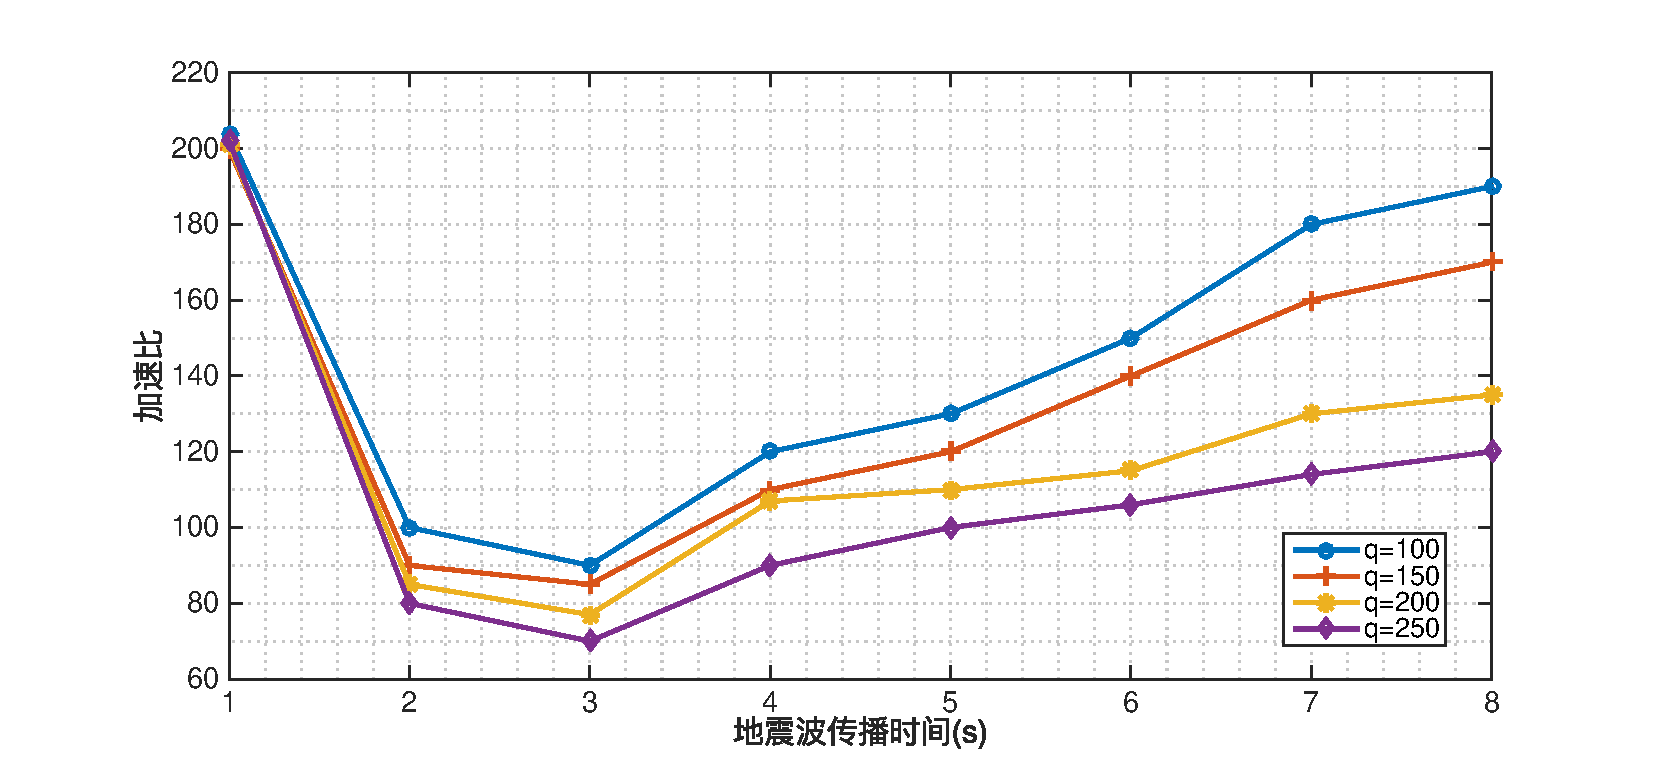
\includegraphics[width=0.9\columnwidth]{不同Q的加速比.eps}
\caption{不同Q在地震波传播不同时间点的加速比。}
\label{fig:diffqspeedup}
\end{figure}


不同优化方法对性能的影响

\section{本章小结}

%\chapter{基于十亿亿次神威超算的高分辨率唐山大地震模拟}
\label{chap:earthquake}

\section{背景知识和算法概述}

在中国传统文化中,对学者的最高评价是“上知天文,下知地理”。自然科学与技术在上世纪取得了长足的进步,然而,地球内部的构造、运动模式、可预测性等问题对于科学家来说仍旧充满未知与神秘。因此,地震等对人类社会生命财产安全造成巨大损失的重大灾害则成为了等待着科学家破译的最终科学挑战之一。

公元132年,东汉著名天文学家张衡设计的地动仪可能是中国历史上最早的抗震减灾科学工作之一(如图所以)。地动仪有八个方位,每个方位上均有口含龙珠的龙头,在每条龙头的下方都有一只蟾蜍与其对应。任何一方如有地震发生,该方向龙口所含龙珠即落入蟾蜍口中,由此便可测出发生地震的方向\cite{}。

这个约在两千年前发明的地动仪中,


有八条龙在他们的嘴里叼着球,能够在千里之外的地震中发现,并展现出与现代地震相似的技术特征 测量仪器起源于1880年代

张衡所设计的地震仪, 如图所示,citep {milne1886earthquakes}。

\section{地震模拟软件框架}


%\include{data/chap02}


%%% 其它部分
\backmatter

%% 本科生要这几个索引,研究生不要。选择性留下。
% 插图索引
%\listoffigures
% 表格索引
%\listoftables
% 公式索引
%\listofequations


%% 参考文献
% 注意:至少需要引用一篇参考文献,否则下面两行可能引起编译错误。
% 如果不需要参考文献,请将下面两行删除或注释掉。
% 数字式引用
\bibliographystyle{thuthesis-numeric}
% 作者-年份式引用
% \bibliographystyle{thuthesis-author-year}
\bibliography{ref/refs}


%% 致谢
%!TEX root = main.tex
% 如果使用声明扫描页,将可选参数指定为扫描后的 PDF 文件名,例如:
% \begin{acknowledgement}[scan-statement.pdf]
\begin{acknowledgement}

衷心感谢我的导师付昊桓老师一直以来对我的栽培,付老师不仅在学术上给我指导、答疑解惑、修改论文、协调资源,他的人格魅力以及待人处事的风格更是深深影响着我。特别感谢杨广文老师对我的悉心照顾,在学习和生活中替我争取了许多锻炼的机会。

毕业论文的顺利完成,离不开所有帮助过我的老师与同学。感谢来自清华的黄小猛老师、薛巍老师和刘利老师学术与科研中不断给予我帮助,答疑解惑,鼓励与启发;感谢国际超级计算无锡中心为我的研究工作提供超算平台与优化建议;感谢伦敦帝国理工学院的Wayne Luk教授、Maxeler公司的Oskar Mencer、斯坦福大学的Robert Clapp研究员给我提供访学交流的机会,并在异构高性能计算和地球物理勘探领域给我许多指导;感谢南方科技大学陈晓非院士研究组和美国圣地亚哥地震中心在我开发大规模唐山大地震模拟中提供了宝贵的建议;感谢所有一起并肩奋斗的同学,甘霖、陈宇澍、赵文来、阮华斌、胡勇、王英侨、魏腾鹏、陈宇澍、薛志辉、廖俊锋、吕子鈜、徐世真、郑伟杰、靳梦瑶、刘邦天、徐敬蘅、刘加贺、方佳瑞、李唯嘉、陈炳伟、张赫、魏衍雯、刘策文、陈悦等等。

感谢我的家人与朋友,特别是李唯嘉,他们一直都是我人生道路中的坚强后盾,也是我不断探知求索的最大动力源泉。

感谢答辩委员会专家及匿名评审专家的宝贵时间和指导。
\end{acknowledgement}


%% 附录
%\begin{appendix}
%\input{data/appendix01}
%\end{appendix}

%% 个人简历
%!TEX root = main.tex
\begin{resume}

  \resumeitem{个人简历}

  1990 年 9 月 13 日出生于广东省兴宁县。

  2009 年 9 月考入中山大学软工学院软件工程专业,2013 年 7 月本科毕业并获得工学学士学位。

  2013 年 9 月免试进入清华大学计算机科学与技术系攻读博士学位至今。

  博士在读期间,2016 年 6 月至 2016 年 9 月在斯坦福大学(Stanford University)地球物理系做访问研究;2016 年 11 月至 2017 年 5 月在伦敦帝国理工学院(Imperial College London)计算机系做访问研究。

  \researchitem{发表的学术论文} % 发表的和录用的合在一起

  % 1. 已经刊载的学术论文(本人是第一作者,或者导师为第一作者本人是第二作者)
  \begin{publications}
    \item Haohuan Fu, \textbf{Conghui He}, Bingwei Chen et al. ``18.9-Pflops Nonlinear Earthquake Simulation on Sunway TaihuLight : Enabling Depiction of 18-Hz and 8-Meter Scenarios." In High Performance Computing, Networking, Storage and Analysis, SC17, 2017. (CCF 推荐 A 类会议,获得2017年“戈登贝尔”奖,本人为通信作者之一)

    \item \textbf{Conghui He}, Haohuan Fu, Ce Guo, Wayne Luk, and Guangwen Yang. ``A Fully-Pipelined Hardware Design for Gaussian Mixture Models." IEEE Transactions on Computers, 2017. (CCF 推荐 A 类期刊)

    \item Haohuan Fu, \textbf{Conghui He}, Huabin Ruan, Itay Greenspon, Wayne Luk, Yongkang Zheng, Junfeng Liao, Qing Zhang, and Guangwen Yang. ``Accelerating Financial Market Server through Hybrid List Design (abstract only)." In Proceedings of the 2017 ACM/SIGDA International Symposium on Field-Programmable Gate Arrays, pp. 289-290. (CCF 推荐 B 类会议)

    \item \textbf{Conghui He}, Haohuan Fu, Wayne Luk, Weijia Li, and Guangwen Yang. ``Exploring the Potential of Reconfigurable Platforms for Order Book Update." In IEEE International Conference on Field-Programmable Logic and Applications (FPL), 2017. (CCF 推荐 C 类会议)

    \item Haohuan Fu, \textbf{Conghui He}, Wayne Luk, Weijia Li, and Guangwen Yang. ``A Nanosecond-level Hybrid Table Design for Financial Market Data Generators." The 25th IEEE International Symposium on Field-Programmable Custom Computing Machines, 2017. (CCF 推荐 C 类会议)

   
  \end{publications}

  % 2. 尚未刊载,但已经接到正式录用函的学术论文(本人为第一作者,或者
  %    导师为第一作者本人是第二作者)。
  % \begin{publications}[before=\publicationskip,after=\publicationskip]
  %   \item Yang Y, Ren T L, Zhu Y P, et al. PMUTs for handwriting recognition. In
  %     press. (已被 Integrated Ferroelectrics 录用. SCI 源刊.)
  % \end{publications}

  % 3. 其他学术论文。可列出除上述两种情况以外的其他学术论文,但必须是
  %    已经刊载或者收到正式录用函的论文。
  \begin{publications}
        \item Weijia Li, \textbf{Conghui He}, Wayne Luk and Haohuan Fu. ``An FPGA-based tree crown detection approach for remote sensing images." The IEEE International Conference on Field-Programmable Technology, 2017. (CCF 推荐 C 类会议)

 \item \textbf{Conghui He}, Haohuan Fu, Yi Shen, Robert Clapp, and Guangwen Yang. ``Ensemble Full Wave Inversion with Source Encoding." In 79th EAGE Conference and Exhibition 2017. 

    \item \textbf{Conghui He}, Yushu Chen, Haohuan Fu, and Guangwen Yang. Ensemble Full Wave Inversion with Source Encoding. In 77th EAGE Conference and Exhibition 2015.

    \item \textbf{Conghui He}, Haohuan Fu, Bangtian Liu, Huabin Ruan, Guangwen Yang, Hui Yang, and Are Osen. ``A GPU-based Parallel Beam Migration Design." In 2015 SEG Annual Meeting. Society of Exploration Geophysicists, 2015.

    \item Bingwei Chen, \textbf{Conghui He}, Yushu Chen, Haohuan Fu. ``Full Wave Inversion Based on EnKF and Source Encoding" In 2016 SEG Annual Meeting. Society of Exploration Geophysicists.

    \item Haohuan Fu, Junfeng Liao, Wei Xue, Lanning Wang, Dexun Chen, Long Gu, Jinxiu Xu, Nan Ding, Xinliang Wang, \textbf{Conghui He}, Shizhen Xu, et al. ``Refactoring and optimizing the community atmosphere model (CAM) on the sunway taihulight supercomputer." Proceedings of the International Conference for High Performance Computing, Networking, Storage and Analysis. IEEE Press, 2016. (CCF 推荐 A 类会议)

    \item Yushu Chen, Guangwen Yang, Xiao Ma, \textbf{Conghui He}, and Guojie Song. ``A time-space domain stereo finite difference method for 3D scalar wave propagation." Computers \& Geosciences 96 (2016): 218-235. (SCI检索)

    \item Nicholas Clinton, Le Yu, Haohuan Fu, \textbf{Conghui He}, and Peng Gong. ``Global-Scale Associations of Vegetation Phenology with Rainfall and Temperature at a High Spatio-Temporal Resolution." Remote Sensing 6, no. 8 (2014): 7320-7338. (SCI检索)
  \end{publications}

  % \researchitem{研究成果} % 有就写,没有就删除
  % \begin{achievements}
  %   \item 任天令, 杨轶, 朱一平, 等. 硅基铁电微声学传感器畴极化区域控制和电极连接的
  %     方法: 中国, CN1602118A. (中国专利公开号)
  %   \item Ren T L, Yang Y, Zhu Y P, et al. Piezoelectric micro acoustic sensor
  %     based on ferroelectric materials: USA, No.11/215, 102. (美国发明专利申请号)
  % \end{achievements}

\end{resume}


%% 本科生进行格式审查是需要下面这个表格,答辩可能不需要。选择性留下。
% 综合论文训练记录表
%\includepdf[pages=-]{scan-record.pdf}
\end{document}
